%% ----------------------------------------------------------------
%% Thesis.tex -- MAIN FILE (the one that you compile with LaTeX)
%% ---------------------------------------------------------------- 

% Set up the document
\documentclass[a4paper, 12pt, oneside]{Thesis}  % Use the "Thesis" style, based on the ECS Thesis style by Steve Gunn
\graphicspath{Figures/}  % Location of the graphics files (set up for graphics to be in PDF format)

% Include any extra LaTeX packages required
\usepackage[square, numbers, comma, sort&compress]{natbib}  % Use the "Natbib" style for the references in the Bibliography
\usepackage[utf8]{inputenc}
\usepackage{vntex} % Vietnamese Typeset for Latex
\usepackage{tikz}
\usepackage{tikz-qtree}
\usepackage{multicol}
\usepackage{multirow}
\usepackage{hyperref}
\usepackage{graphicx}
\usepackage{float}
\usepackage{pifont}% http://ctan.org/pkg/pifont
\newcommand{\cmark}{\ding{51}}%
\newcommand{\xmark}{\ding{55}}%
\usepackage{verbatim}  % Needed for the "comment" environment to make LaTeX comments


\usepackage{fancyvrb}
\usepackage{vector}  % Allows "\bvec{}" and "\buvec{}" for "blackboard" style bold vectors in 
\hypersetup{urlcolor=blue, colorlinks=true}  % Colours hyperlinks in blue, but this can be distracting if there are many links.
%% ----------------------------------------------------------------
%% fill a page with dotlines 
\makeatletter

\newlength\dottedlinefillheight
\setlength\dottedlinefillheight{.25in}

\newcommand\fillwithdottedlines[1]{%
	\begingroup
	\ifhmode
	\par
	\fi
	\hrule height \z@
	\nobreak
	\setbox0=\hbox to \hsize{\hskip \@totalleftmargin
		\vrule height \dottedlinefillheight depth \z@ width \z@
		\dotfill}%
	% We use \cleaders (rather than \leaders) so that a given
	% vertical space will always produce the same number of lines
	% no matter where on the page it happens to start:
	\cleaders \copy0 \vskip #1 \hbox{}%
	\endgroup
}
\makeatother
%% ----------------------------------------------------------------
\begin{document}
\frontmatter      % Begin Roman style (i, ii, iii, iv...) page numbering
\lhead{}
% Set up Bìa chính
\title{\textbf{HỆ THỐNG PHÂN LOẠI TỰ ĐỘNG}}
%\supervisor{\texorpdfstring{TS. Nguyễn Anh Tuấn{Supervisor Name}}}
\examiner    {}
\degree      {}
\authors  {\texorpdfstring
            {ĐẶNG LÊ BẢO CHƯƠNG}{Author Name}
            \\
            \texorpdfstring
            {NGUYỄN BẢO DUY}{Author Name}
            }
\addresses  {\groupname\\\deptname\\\univname}  % Do not change this here, instead these must be set in the "Thesis.cls" file, please look through it instead
\date       {\today}
\subject    {}
\keywords   {}
%% ----------------------------------------------------------------
% Bìa chính
%% ----------------------------------------------------------------
\maketitle
\authors  {\texorpdfstring
	{ĐẶNG LÊ BẢO CHƯƠNG - 10520010}{Author Name}
	\\
	\texorpdfstring
	{NGUYỄN BẢO DUY - 10520011}{Author Name}
}
%% ----------------------------------------------------------------
% Bìa phụ
%% ----------------------------------------------------------------
\makesubtitle
%% ----------------------------------------------------------------
% Danh sách hội đồng phản biện
%% ----------------------------------------------------------------
\dshoidong
%% ----------------------------------------------------------------
% Nhận xét của giáo viên hướng dẫn
%% ----------------------------------------------------------------
\nhanxet{Cán bộ hướng dẫn}{TS. Nguyễn Anh Tuấn}
%% ----------------------------------------------------------------
% Nhận xét của giáo viên phản biện
%% ----------------------------------------------------------------
\nhanxet{Cán bộ phản biện}{\dotfill}
%% ----------------------------------------------------------------
% Lời cảm ơn
%% ----------------------------------------------------------------
\acknowledgements{	
\hspace*{0.05\textwidth}Đầu tiên, chúng em xin chân thành cám ơn Khoa Mạng máy tính và Truyền thông, trường Đại Học Công Nghệ Thông Tin, Đại Học Quốc Gia TP.HCM đã tạo điều kiện cho chúng em hoàn thành tốt khoá luận này.
\\
Chúng em xin chân thành cám ơn Thầy Nguyễn Anh Tuấn, đã tận tình hướng dẫn, dạy dỗ, chỉ bảo chúng em từ những ngày đầu định hình khoá luận cho đến khi hoàn thành. Nhờ sự tận tình của thầy, chúng em đã hoàn thành tốt khoá luận này, bên cạnh đó cũng học hỏi được nhiều kiến thức quý báu từ thầy.
\\
Chúng em xin chân thành cảm ơn quý Thầy Cô trong Khoa Mạng máy tính và truyền thông, trong những năm qua đã không quản ngại mệt mỏi, tận tình giảng dạy, trang bị cho chúng em những kiến thức cần thiết để hoàn thành khoá luận.
\\
Chúng em xin ghi nhớ công ơn sinh thành dưỡng dục của cha mẹ, sự giúp đỡ của các anh, chị, bạn bè trong những năm học, cũng như sự an ủi, động viên trong những lúc khó khăn, vất vả. Dù chúng em đã dùng tất cả nỗ lực của bản thân để hoàn thành tốt khoá luận này, tuy nhiên không thể tránh khỏi những sơ suất, thiếu sót. Kính mong quý Thầy Cô tận tình chỉ bảo. Một lần nữa, chúng em xin chân thành cảm ơn và mong nhận được nhiều tình cảm chân thành của tất cả mọi người.	
}
%% ----------------------------------------------------------------
% Đề cương chi tiết
%% ----------------------------------------------------------------
\decuongB
%% ----------------------------------------------------------------
\setstretch{1.3}  % Reset the line-spacing to 1.3 for body text (if it has changed)
\pagestyle{fancy}  %The page style headers have been "empty" all this time, now use the "fancy" headers as defined before to bring them back
%% ----------------------------------------------------------------
% 	Mục lục
%% ----------------------------------------------------------------
%\lhead{\emph{Mục lục}}  % Set the left side page header to "Contents"
\tableofcontents
%% ----------------------------------------------------------------
\pagestyle{empty}
% 	Danh sách hình vẽ
%% ----------------------------------------------------------------
%\lhead{\emph{Danh sách hình vẽ}}  % Set the left side page header to "List of Figures"
\listoffigures 
%% ----------------------------------------------------------------
% 	Danh sách bảng
%% ----------------------------------------------------------------
%\lhead{\emph{Danh sách các bảng}}  % Set the left side page header to "List of Tables"
\listoftables 
%% ----------------------------------------------------------------
\setstretch{1.5}  % Set the line spacing to 1.5, this makes the following tables easier to read
\clearpage  % Start a new page
%\lhead{\emph{Danh sách các từ viết tắt}}  % Set the left side page header to "Abbreviations"
%% ----------------------------------------------------------------
% 	Danh sách từ viết tắt
%% ----------------------------------------------------------------
\listofsymbols{ll}  % Include a list of Abbreviations (a table of two columns)
{
	% Từ viết tắt 		% Tên đầy đủ
	\textbf{OWL2} 		& \textbf{O}ntology \textbf{W}eb \textbf{L}anguage \textbf{2}\\
	\textbf{SWRL} 		& \textbf{S}emantic \textbf{W}eb \textbf{R}ule \textbf{L}anguage\\
	\textbf{CWA} 		& \textbf{C}losed \textbf{W}orld \textbf{A}ssumption\\
	\textbf{OWA} 		& \textbf{O}pen \textbf{W}orld \textbf{A}ssumption\\
	\textbf{RDF} 		& \textbf{R}esource \textbf{D}escription \textbf{F}ramework\\
	\textbf{XML}		& e\textbf{X}tensible \textbf{M}arkup \textbf{L}anguage\\
	\textbf{IRI}		& \textbf{I}nternationalized \textbf{R}esource \textbf{I}dentifier\\
%	\textbf{KB} 		& \textbf{K}nowledge \textbf{B}ase\\
%	\textbf{KR} 		& \textbf{K}nowledge \textbf{R}epresentation\\
	\textbf{DL} 		& \textbf{D}escription \textbf{L}ogic\\
%	\textbf{MUPS} 		& \textbf{M}inimal \textbf{U}nsatisfiability \textbf{P}reserving \textbf{S}ub-TBoxes\\
%	\textbf{HST} 		& \textbf{H}itting \textbf{S}et \textbf{T}ree\\
%	\textbf{HS} 		& \textbf{H}itting \textbf{S}et\\
}
%% ----------------------------------------------------------------
% 	Danh sách ký hiệu
%% ----------------------------------------------------------------
%\listofnomenclature{lll}  % Include a list of Symbols (a three column table)
%{
%	% symbol 		% explanation						% giải thích
%	$\models$ 		& models of 						& có nghĩa trong (KB)\\
%	$\not\models$ 	& not a model  of 					& không có nghĩa trong KB\\
%	$\subseteq$ 	& is a subset of 					& là tập con của\\
%	$\cap$ 			& intersect 						& giao với\\
%	$\neg$ $A$ 		& complement of A of 				& không phải A\\
%	$\exists$ $R.E$ & e.g \textit{has} some E 			& \\
%	$\forall$ $R.E$ & e.g \textit{has} only E 			& \\
%	$\equiv$ 		&  is equivalent to 				& tương đương với \\
%	$\emptyset$ 	& empty set 						& tập hợp rỗng \\
%	$\in$ 			& is member of	 					& thuộc \\
%	$\Leftarrow$ 	& preferred for left implication 	& \\
%	$\backslash$ 	& except 							& ngoại trừ \\
%	& & \\
%}
%% ----------------------------------------------------------------
%% Lời mở đầu
%% ----------------------------------------------------------------
\openingwords{
%\addtocontents{toc}{\vspace{1em}}
Thế giới của chúng ta đang liên tục vận động theo chiều hướng tích cực. Đây là nguyên nhân chủ yếu cho sự phát triển và thay đổi hằng ngày của mọi lĩnh vực đời sống, đặc biệt là khoa học công nghệ nói chung, và ngành công nghệ thông tin nói riêng. Hiện nay, hầu hết mọi nơi trên thế giới đều đã biết đến sự có mặt của công nghệ thông tin, máy tính, và kể cả internet. Việc internet ra đời là một sự kiện đã làm thay đổi cả thế giới. Thay thế cho việc gọi điện thoại hằng ngày, chúng ta có thể liên lạc qua internet, với việc có thể thấy được hình ảnh của người đối diện chứ không chỉ riêng giọng nói. Thay thế cho những tờ báo bằng giấy, chúng ta đã có những trang web, với những thông tin đầy đủ hơn, hình ảnh sinh động hơn, và cả những đoạn video minh hoạ. Những thông tin trên internet được lan truyền với tốc độ chóng mặt, dẫn đến việc những tin tức nóng nhất được cập nhật liên tục trong từng phút từng giây. Cách tiếp cận thông tin của con người thay đổi, nên sự chuyển động của thông tin ngày càng nhanh hơn, và đến mức nào đó, thông tin sẽ không mang theo đủ những gì mà con người mong muốn truyền tải. Đó là lúc mà con người nghĩ đến việc thay đổi. Và đó cũng chính là lúc Semantic Web được ra đời. Semantic Web mang sứ mệnh lớn lao trong việc thay đổi công nghệ web. Trước đây, máy tính chỉ đóng vai trò là trung tâm “chứa đựng” và “duy trì” các trang web. Tuy nhiên, với Semantic Web, máy tính sẽ phải làm nhiều hơn thế, sẽ phải “suy nghĩ” và “sử dụng” trang web một phần nào đó thay thế cho con người. Để làm được điều này không phải dễ dàng, vì máy tính là vật vô tri vô giác. Do đó, một cách tiếp cận đơn giản để giải quyết vấn đề này, bằng cách thêm vào các trang web thông thường metadata, để các máy tính có thể “đọc” được, như một ngôn ngữ chung của các máy tính. 
\\
Nhận thấy được những tiềm năng và những lợi ích to lớn của Semantic Web, chúng em đã lựa chọn đề tài này. Trước tiên, chúng em đã tập trung nghiên cứu và tìm hiểu sâu hơn về Semantic Web, cụ thể hơn là ngôn ngữ OWL2, và SWRL Rule. Ứng dụng của Semantic Web và Ontology rất đa dạng và phong phú. Mục đích chính của nhóm hướng đến việc chứng minh tính khả thi của việc sử dụng kết hợp ngôn ngữ OWL, SWRL Rule và hoạt động của reasoner trong việc phân loại tự động cá thể. Sau khi chứng minh được điều đó, chúng em quyết định xây dựng một công cụ chỉnh sửa ontology trên web, vì nhận thấy chưa có một công cụ nào đáp ứng được nhu cầu đó. Sau đó chúng em sẽ tiếp tục phát triển hơn khả năng phân loại tự động đó trong từng lĩnh vực cụ thể, chẳng hạn như việc phân loại hàng hoá xuất nhập khẩu tại các cảng hải quan, hay việc phân loại các gói tin trong lưu lượng mạng...
\\
Trong quá trình nghiên cứu và phát triển ứng dụng, tuy gặp phải những khái niệm và công nghệ hoàn toàn mới lạ và ít được công bố, chúng em vẫn cố gắng tìm hiểu bằng mọi cách. Sau hơn 6 tháng làm việc, kết quả đạt được của nhóm là một chương trình chỉnh sửa file Ontology trên nền tảng web, tích hợp khả năng phân loại tự động các cá thể. Hơn nữa, điều này cũng chứng minh tính khả thi trong việc áp dụng công nghệ ontology vào trong việc phân loại tự động các đối tượng thực tế.
\\
Lĩnh vực Semantic Web là rất rộng lớn, với một khoảng thời gian có hạn, chúng em chỉ có thể tìm hiểu được những vấn đề được coi là cơ bản và tất yếu nhất của Semantic Web và Ontology. Dù vậy, chúng em rất hài lòng và tự tin với những gì tìm hiểu, nghiên cứu và phát triển được sẽ mang lại nhiều lợi ích, đóng góp vào công cuộc nghiên cứu khoa học chung.	
}
%% ----------------------------------------------------------------
%% Quy ước khóa luận của trường Đại học Công Nghệ Thông Tin
%% ----------------------------------------------------------------
\clearpage  %Start a new page
\setmarginsrb           { 3.5cm}  % left margin
						{ 2.0cm}  % top margin
						{ 2.0cm}  % right margin
						{ 2.5cm}  % bottom margin
						{ 1.0cm}  % head height
						{ 0.5cm}  % head sep
						{ 1.0cm}  % foot height
						{ .75cm}  % foot sep
\mainmatter	  % Begin normal, numeric (1,2,3...) page numbering
\pagestyle{fancy}  % Return the page headers back to the "fancy" style
\lhead{}
\cfoot{\thepage}
% Include the chapters of the thesis, as separate files
% Just uncomment the lines as you write the chapters
%% ----------------------------------------------------------------
%% Nội dung khóa luận
%% ----------------------------------------------------------------
\chapter {Giới thiệu đề tài}
\section{Tên đề tài}
Trình biên soạn Ontology 
\section{Nội dung và giới hạn đề tài}
\subsection{Nội dung đề tài}
OWL ( Web Ontology Language ) là một dạng ngôn ngữ biểu diễn tri thức. Ngôn ngữ này thường được sử dụng phổ biến trong Semantic Web, và được trình bày dưới dạng RDF-XML. Ngày 27 tháng 10 năm 2009, tổ chức W3C (World Wide Web Consortium) cho công bố OWL 2, với trình chỉnh sửa Protégé và các bộ reasoner như Pellet, HermiT, v.v .
\\
OWL và Semantic Web hiện đang được nghiên cứu và phát triển, nhằm nhanh chóng đưa vào sử dụng, vì những lợi ích rất đáng kể của nó, được ví như là công nghệ web phiên bản 3.0. Do đó, nhóm quyết định nghiên cứu về OWL, về phương thức hoạt động của các bộ reasoner, và đặc biệt là thiết kế một trình chỉnh sửa OWL trên web với giao diện thân thiện và dễ sử dụng, với các tính năng gần như đầy đủ so với chương trình Protégé. 
\\
Chắc chắn trong vài năm sắp tới, Semantic Web sẽ phát triển ngày càng lớn mạnh hơn, dần dần thay đổi phương thức tiếp cận và lưu trữ dữ liệu trên web. Vậy nên, việc tìm hiểu và nghiên cứu về ngôn ngữ OWL - một trong những thành phần quan trọng của Semantic Web, có thể coi như một bước “đón đầu công nghệ”, nhằm mục đích sẵn sàng thích nghi với sự chuyển biến không ngừng của thế giới công nghệ thông tin.
\\
Đề tài sẽ làm những việc sau:
\begin{enumerate}
\item Tìm hiểu về Semantic Web.
\item Tìm hiểu về ngôn ngữ Web Ontology Language (OWL) và Semantic Web Rule Language(SWRL).
\item Tìm hiểu về OWLAPI và SWRL API.
\item Tìm hiểu về nguyên lý hoạt động của OWL Reasoner (cụ thể là Pellet Reasoner).
\item Tìm hiểu về Vaadin Framework.
\item Sử dụng Vaadin Framework để xây dựng công cụ phục vụ phát triển Ontology trên web.
\item Giới thiệu những đặc điểm và tính năng nổi bật của phần mềm.
\item Kết luận và hướng phát triển nghiên cứu.
\end{enumerate}
\subsection{Giới hạn của đề tài}
Lĩnh vực Semantic Web là rất rộng lớn, 

\subsection{Cấu trúc luận văn}
Luận văn được chia thành các chương như sau : 


\chapter{Cơ sở lý thuyết}
\paragraph{Giới thiệu} Chương này sẽ tập trung giới thiệu từ khái quát đến chi tiết về những đặc tính lý thuyết của Web Ngữ Nghĩa - Semantic Web, ngôn ngữ Ontology Web Language, ngôn ngữ Semantic Web Rule Language (SWRL) và tính nhất quán của ontology - Ontology Consistency. Đây là những nền tảng lý thuyết cơ bản nhất giúp chúng em xây dựng nên hệ thống phân loại tự động. Cuối chương, chúng em xin giới thiệu khái quát về nên tảng và các thư viện lập trình được chúng em sử dụng để xây dựng hệ thống.

%% ----------------------------------------------------------------
% 	Semantic Web
%% ----------------------------------------------------------------
\section{Semantic Web}
Như chúng ta đã biết hệ thống Web hiện tại mà chúng ta được sử dụng được gọi là Web 2.0 thì Semantic Web hay còn gọi là Web ngữ nghĩa được các nhà nghiên cứu từ tổ chức World Wide Web Consortium (W3C) kỳ vọng sẽ trở thành Web 3.0 trong tương lai gần. Semantic Web khuyến khích tích hợp đặc tính ngữ nghĩa vào các tài nguyên Web hiện có bằng việc đặt ra mục tiêu chuyển đổi hệ thống Web hiện tai - vốn được hình thành từ những dữ liệu không được tổ chức hoặc chỉ được tổ chức một phần - thành một tập hợp dữ liệu, tài nguyên thống nhất (A Web of Data). Để làm được việc đó, tổ chức W3C đó đề ra những quy ước chung cho các thành phần của Semantic Web. Mục tiêu cuối cùng mà Semantic Web như trong phát biểu của ngài Tim Berners-Lee - người phát minh ra WWW: "Semantic Web cung cấp một bộ công cụ thống nhất (framework) để dữ liệu có thể được chia sẻ, tái sử dụng giữa các ứng dụng với nhau, giữa các doanh nghiệp, tổ chức hay trong cộng đồng người dùng web với nhau" \cite{semantic3}. Sau đây, chúng em xin giới nguyên lý và các thành phần của Semantic Web.
%. với đặc trưng riêng biệt là phương thức liên kết dữ liệu (linked data) giữa các hệ thống hoặc các thực thể cho phép thể hiện được nhiều hơn, và rõ ràng hơn mối liên kết giữa các dữ liệu trên mạng lưới web toàn cầu. Cụ thể hơn, Semantic Web có khả năng chuyển đổi văn bản HTML của con người (human readable HTML documents) sang ngôn ngữ máy tính (machine readable documents), giúp cho máy tính làm được nhiều công việc suy nghĩ hơn cho con người \cite{semantic1}. 
%\\
%Ngày nay, đa phần dữ liệu trên web được cung cấp dưới dạng trang web (web pages) - văn bản HTML được liên kết với nhau bằng các liên kết (hyperlinks). Cả người và máy tính đều có thể dễ dàng đọc hiểu những văn bản đó, tuy nhiên thay vì dễ dàng tìm kiếm những từ khoá trong trang web, máy tính lại gặp trở ngại khi chọn lọc những ý nghĩa trong các văn bản đó. Một trang web chứa rất nhiều thông tin, nhưng những thông tin đó không phải là những thông tin thô - mà chỉ là những văn bản HTML được xây dựng từ cơ sở dữ liệu. Vậy nên Semantic Web đã thay đổi hướng nhìn và đưa ra giải pháp cho vấn đề ở trên theo nhiều cách khác nhau :
%\begin{itemize}
%	\item Chuyển những trang web dữ liệu thành những tiến trình xử lý thông minh nhân tạo (giúp trang web phải “suy nghĩ” để xử lý giúp con người).
%	\item Khuyến khích các công ty, các doanh nghiệp và các cá nhân trình bày dữ liệu tự do hơn, theo một quy chuẩn mở.
%	\item Khuyến khích các doanh nghiệp sử dụng dữ liệu đã có sẵn trên web.
%\end{itemize}
 
\subsection{Semantic Web dựa trên giả định thế giới mở (Open World Assumption)} 
Với đặc điểm của thông tin trên Web là những thông tin luôn luôn cần được thêm vào hay chỉnh sửa (thông tin trên web cũng giống như kiến thức vì thế nó sẽ không bao giờ bị giới hạn) nên thay vì chọn tuân theo giả định thế giới đóng (Closed World Assumption - CWA), vốn đã tồn tại rất lâu trong các cơ sở dữ liệu quan hệ (SQL), các nhà nghiên cứu đã chọn giả định thế giới mở làm nguyên lý cho mọi lý thuyết và định nghĩa của Semantic Web. Một so sánh ngắn gọn giữa giả định Thế Giới Mở (Open World Assumption - OWA)\cite{OWA_0} được Semantic Web chấp nhận và giả định Thế Giới Đóng (CWA).
\begin{description}
	\item[Closed World Assumption] 
	Giả định Thế Giới Đóng (CWA) là giả định mà những điều không chắc hoặc không có cơ sở để chứng minh là \textbf{đúng} sẽ được chấp nhận là \textbf{sai}.
	\item[Open World Assumption]
	Giả định Thế Giới Mở (OWA) thì ngược lại, với những điều không chắc hoặc không có cơ sở để chứng minh là \textbf{đúng} sẽ được chấp nhận là \textbf{chưa biết}. 
	\item[Ví dụ]
	Xem xét một câu nói sau đây: "A là một công dân của nước Hoa Kỳ". Nếu có ai đó hỏi "A có phải là một công dân của Việt Nam hay không ?". Xét theo CWA, câu trả lời là \textit{không}, ngược lại với OWA thì câu trả lời là \textit{chưa biết}. 
\end{description}
%
\subsection{Các thành phần của Semantic Web}
Khái niệm "Semantic Web" thường được sử dụng cụ thể hơn nhằm chỉ đến những định dạng và công nghệ để hiện thực hóa nó. Việc tổ chức, tập hợp và phục hồi dữ liệu liên kết thực hiện được nhờ vào các công nghệ đặc tả chính thức về các khái niệm, định nghĩa và mối quan hệ trong một lĩnh vực tri thức được biết đến. Tất cả các công nghệ này đều được quy định thành một tiêu chuẩn của tổ chức World Wide Web Consortium (W3C) . Các tiêu chuẩn được liệt kê trong \cite{semantic2} và dựa vào các thành phần đó các nhà nghiên cứu đã đưa ra các thành phần của Semantic Web như sau
\begin{figure}[h!]
	\centering
	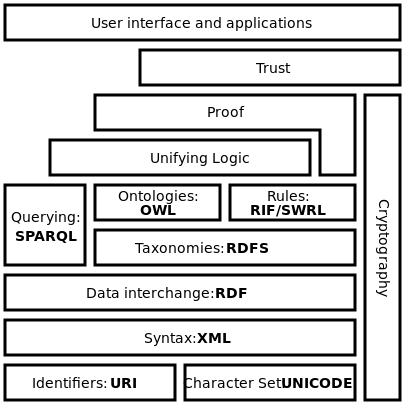
\includegraphics[width=110mm]{Figures/semantic_web_stack.png}
	\caption{The Semantic Web Stack \label{overflow}}
\end{figure}
%\begin{itemize}
%	\item \href{http://en.wikipedia.org/wiki/Resource\_Description\_Framework}{Resource Description Framework}, một phương thức chung để biểu diễn thông tin cho semantic web.
%	\item \href{http://en.wikipedia.org/wiki/RDF_Schema}{RDF Schema}
%	\item \href{http://en.wikipedia.org/wiki/Simple_Knowledge_Organization_System}{Simple Knowledge Organization System} (SKOS)
%	\item \href{http://en.wikipedia.org/wiki/SPARQL}{SPARQL} - Ngôn ngữ truy vấn dữ liệu biểu diễn dưới dạng RDF.
%	\item \href{http://en.wikipedia.org/wiki/Notation3}{Notation3}, thiết kế với tiêu chí hiểu được bởi con người.
%	\item \href{http://en.wikipedia.org/wiki/N-Triples}{N-Triples}, một định dạng dùng để lưu và truyền dữ liệu.
%	\item \href{http://en.wikipedia.org/wiki/Turtle_(syntax)}{Turtle} (Terse RDF Triple Language)
%	\item \href{http://en.wikipedia.org/wiki/Web_Ontology_Language}{Web Ontology Language} (OWL), một họ các ngôn ngữ biểu diễn tri thức.
%	\item \href{}{Rule Interchange Format} (RIF), một framework chung của các ngôn ngữ điều luật web hỗ trợ chuyển đổi nhiều điều luật khác nhau trên web.
%\end{itemize}

Hình Semantic Web Stack \cite{semantic3} miêu tả kiến trúc của Semantic Web:
\begin{enumerate}
	\item \textbf{XML} là định dạng tài liệu chính để lưu trữ các mô hình dữ liệu, thông tin mà Semantic Web diễn đạt. Ngoài XML cũng tồn tại các định dạng thay thế khác như Turle \textsuperscript{*}. 
	\item \textbf{XML Schema} quy định tiêu chuẩn cho các tài liệu Semantic Web, có thể ví nó như phần mở rộng trong tên tập tin, giúp phân biệt các tiêu chuẩn, các loại tài liệu Semantic khác nhau như OWL/XML, RDF/XML.
	\item \textbf{Resource Description Framework} (RDF) \cite{rdf} là ngôn ngữ đầu tiên được quy định bởi W3C để diễn tả các mô hình dữ liệu và mối quan hệ của chúng. RDF có thể được lưu trữ dưới nhiều dạng định dạng khác nhau  ví dụ như: RDF/XML, N3, Turtle và RDFa. Có thể nói RDF chính là thành phần cơ bản và quan trọng nhất của Semantic Web.
	\item \textbf{RDF Schema} (RDFS) \cite{rdfs} mở rộng RDF bằng những vốn từ vựng mới dùng miêu tả các thuộc tính và phân lớp trong các tài nguyên web hay mô hình dữ liệu được biểu diễn bằng RDF.
	\item \textbf{Ontology Web Language} (OWL) là ngôn ngữ với cú pháp hoàn toàn mới dùng với mục tiêu tương tự RDFS, tuy nhiên ngoài việc biểu diễn được lớp, thuộc tính như RDFS, OWL còn có khả năng các mối quan hệ giữa các đối tượng trong mô hình dữ liệu chi tiết hơn nhiều. Ví dụ: quy định các lớp không được phép có chung cá thể nào (disjointness), các phát biểu ràng buộc số lượng (cardinality), cung cấp nhiều loại dữ liệu cho các thuộc tính, và mô tả được thuộc tính bằng các tính chất (đối xứng/ bất đối xứng, và các lớp liệt kê, ...).
	\item \textbf{SPARQL} là một giao thức và ngôn ngữ truy vấn dữ liệu dành cho tài nguyên của Semantic Web (RDF, RDFS, OWL).
	\item \textbf{RIF} (W3C Rule Interchange Format) là một ngôn ngữ XML để biểu diễn điều luật web mà máy tính có thể thực thi.
\end{enumerate}
{\let\thefootnote\relax\footnotetext{*\textit{
			Turtle: http://en.wikipedia.org/wiki/Turtle\_(syntax)}}
}
%% ----------------------------------------------------------------
% 	Kết thúc Semantic Web
%% ----------------------------------------------------------------
% 	Ontology Web Language 
%% ----------------------------------------------------------------
\section{Ontology Web Language 2}
Là một thành phần chính của Semantic Web, nhiệm vụ của Ontology Web Language (OWL) chính là một Semantic Web. OWL được tổ chức W3C khuyến khích sử dụng vì những thành phần từ vựng mới của nó giúp đặc tả các thực thể trong một lĩnh vực nào đó hiệu quả hơn so với RDFS hay RDF. Phiên bản OWL hiện thời là phiên bản 2 \cite{owl2}. Về mặt lý thuyết, OWL là một ngôn ngữ ontology tuân theo Description Logic (DL) $SROIQ_{(D)}$ \cite{DL}, với ưu điểm là ngoài  khả năng đặc tả vừa nêu, nó còn biểu diễn được những suy luận được suy ra từ những đặc tả được khai báo. Khả năng suy luận của OWL chính là điểm quyết định cho tính khả thi của hệ thống phân loại tự động.
\subsection{Đặc điểm tổng quan}
\begin{figure}[h!]
	\centering
	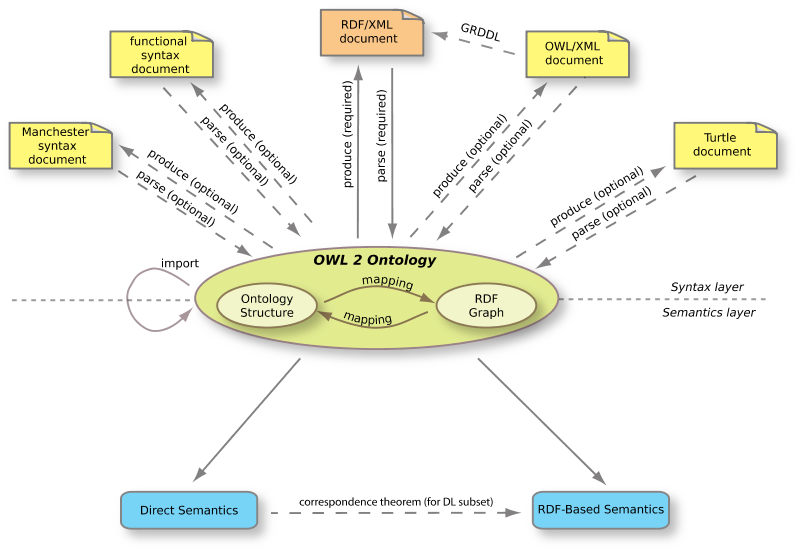
\includegraphics[width=130mm]{Figures/owl2structure.png}
	\caption{Cấu trúc của OWL 2\label{overflow}}
\end{figure}
Hình trên cho chúng ta cái nhìn tổng quan về các định dạng tài liệu, các loại cú pháp và các khả năng chuyển đổi thành RDF Graph của Ontology. Trong hình, hình ê-líp ở giữa thể hiện các khái niệm mà một ontology muốn thể hiện, các thông tin này có khả năng chuyển đổi qua lại thành định dạng đồ thị RDF \cite{mapping_rdf_graph} (RDF Graph - là định dạng chính trong các cơ sở dữ liệu đồ thị ngữ nghĩa). Ontology có thể được biểu diễn dưới nhiều dạng cú pháp và lưu trữ dưới nhiều dạng tài liệu khác nhau (Syntax Layer trong hình), các định dạng và cú pháp này hoàn toàn có thể chuyển đổi qua lại với nhau. Lớp ngữ nghĩa trong hình (Semantic Layer) cho thấy ngữ nghĩa được quy định theo 2 tiêu chuẩn kỹ thuật khác nhau là Direct Semantics và RDF-Based Semantics.
\subsubsection{Cú pháp và định dạng}
Cú pháp cần thiết cho việc biểu diễn hay xây dựng ontology, định dạng cần cho việc lưu trữ và trao đổi giữa các ứng dụng với nhau.Trong OWL, mỗi định dạng tài liệu sẽ gắn liền với một loại tài liệu. Định dạng/cú pháp chính của OWL là RDF/XML [\href{http://www.w3.org/TR/owl2-overview/#ref-rdf-syntax}{RDF Syntax}] \cite{rdfxml}. Ngoài ra, còn có các định dạng/cú pháp khác cũng nằm trong quy định của tổ chức W3C.
%Dưới đây là bảng so sánh và liệt kê các cú pháp.
%\begin{table}[H]
%	\begin{tabular}{ |p{3cm}|p{4cm}|p{2cm}|p{4cm}|}
%		\hline
%		Tên cú pháp & Mô tả & Trạng thái & Mục đích sử dụng\\
%		\hline
%		RDF/XML & Mapping to RDF Graphs \cite{mapping_rdf_graph} \cite{rdfxml} & Bắt buộc & Hoán đổi được ( có thể viết và đọc được bằng nhiều phần mềm OWL2)
%		\\
%		\hline
%		OWL/XML & XML Serialization \cite{owlxml} & Tùy chọn & Xử lý dễ dàng hơn bằng công cụ XML.
%		\\
%		\hline
%		Functional Syntax & Structural Specification \cite{func_syntax} & Tùy chọn & Dễ đọc và hiểu được.
%		\\
%		\hline
%		Manchester Syntax & Manchester Syntax \cite{man_syntax} & Tùy chọn & Có ưu thế hơn để đọc/ghi DL Ontologies
%		\\
%		\hline
%		Turtle & Mapping to RDF Graphs \cite{mapping_rdf_graph} & Tùy chọn, không được công nhận chính thức & Có ưu thế để đọc/ghi RDF triples
%		\\
%		\hline
%	\end{tabular}
%	\caption{Bảng so sánh các cú pháp của OWL2\label{overflow}}
%\end{table}
\subsection{Một số ví dụ của các định dạng/cú pháp khác nhau}

\textbf{Functional Syntax}
\begin{verbatim}
Declaration(Class (Grass))) # Khai báo lớp
Declaration(ObjectProperty (canEat))  # Khái báo thuộc tính
SubClassOf(Cow Animal)  # Khai báo lớp con
\end{verbatim}

\textbf{RDF/XML Syntax}
\begin{verbatim}
T(Animal) rdf:type owl:Class
T(canEat) rdf:type owl:ObjectProperty
T(Cow) rdfs:subClassOf T(Animal) 
\end{verbatim}


\textbf{OWL/XML Syntax}
\begin{verbatim}
<Declaration>
<Class IRI="#Animal"/> // Khai báo lớp
</Declaration>
<Declaration>
<ObjectProperty IRI="#canEat"/> // Khai báo thuộc tính
</Declaration>
<SubClassOf>
<Class IRI="#Cow"/>
<Class IRI="#Animal"/>  // Khai báo lớp con
</SubClassOf>
\end{verbatim}

\textbf{Manchester Syntax}
\begin{verbatim}
Class: Cow  # Khái báo lơp chung với lớp con
	SubClassOf: Animal 
	SubClassOf: canEat some Grass
\end{verbatim}


\subsection{Các thành phần chi tiết của một OWL 2 ontology}

\subsubsection{Ontology IRI và Version IRI}
Mỗi ontology đều có thể gồm \textit{một ontology IRI} \cite{iri} \textsuperscript{*} (Internationalized Resource Identifier), dùng để định danh cho ontology. Nếu một ontology có một ontology IRI, thì ontology này có thể có thêm một version IRI, dùng để xác định phiên bản cho ontology này. Version IRI có thể trùng hoặc không nhất thiết phải trùng với ontology IRI. Một ontology không có ontology IRI thì không có version IRI.
%Dưới đây là những quy ước chọn ontology IRIs và version IRIs trong OWL2. Những đặc điểm kỹ thuật này không cung cấp cơ chế nào để làm chúng phải được tuân theo trên toàn hệ thống web. Tuy nghiên, những công cụ hay ứng dụng OWl2 \textit{nên} sử dụng những quy ước này để dễ dàng tìm ra lỗi trong những ontology mà chúng xử lý.
{\let\thefootnote\relax\footnotetext{*\textit{
			Internationalized Resource Identifier: giao thức bổ sung cho Uniform Resource Universal Character Set (Unicode/ISO 10646).}}
}
%\begin{itemize}
%	\item Nếu một ontology có một ontology IRI nhưng không có version IRI, thì \textit{không nên tồn tại} một ontology với trùng ontology IRI vừa đặt.
%	\item Nếu một ontology có một ontology IRI và một version IRI, thì \textit{không nên tồn tai} một ontology khác với trùng ontology IRI và version IRI vừa đặt.
%	\item Tất cả các cách kết hợp khác của ontology IRI và version IRI không cần đòi hỏi tính duy nhất (unique). Như vậy 2 ontologies khác nhau có thể không có ontology IRI và version IRI; tương tự, một ontology chưa một ontology IRI có thể cùng tồn tại cùng với một ontology khác có cùng ontology IRI vừa đặt \textbf{và} các version IRI của các ontologies này \textbf{phải} khác nhau.
%\end{itemize}
\\
Ontology IRI và các version IRI kết hợp với nhau giúp định danh một phiên bản cụ thể của của ontology từ một bộ chứa tất cả các phiên bản của một ontology cụ thể nào đó được định danh chung bằng ontology IRI. Trong mỗi bộ ontology như vậy, sẽ có chính xác một ontology được xác định như một ontology hiện hành - khi dùng ontology IRI để truy vấn ontology mà không đề cập đến version IRI, mặc định ontology có verison IRI hiện hành sẽ được trả về.


\subsubsection{Thực thể, trực nghĩa và cá thể ẩn danh - Entities, Literals and Anonymous Individuals}
Các thực thể (entities) là thành phần cơ bản nhất của OWL2 Ontology, chúng định nghĩa các từ vựng - cụ thể là những đặt tên ra các khái niệm (named term) - của một ontology. Bên cạnh các thực thể, OWL 2 ontologies thường có thêm các trực nghĩa (literals), như strings hay integers.
\begin{figure}[ht!]
	\centering
	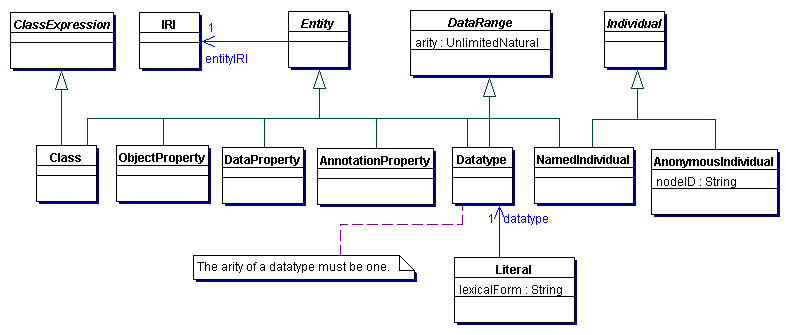
\includegraphics[width=155mm, height=80mm]{Figures/entities.png}
	\caption{Entities, Literals, Anonymous Individuals trong OWL2 \label{overflow}}
\end{figure}
\\
Cấu trúc của các thực thể và trực nghĩa trong OWL 2 được thể hiện trong hình bên. Các lớp (classes), kiểu dữ liệu (datatypes), thuộc tính đối tượng (object properties), thuộc tính dữ liệu (data properties), thuộc tính chú thích và các cá thể có tên đều được gọi chung là các thực thể (entities), tất cả chúng được được định danh bằng một IRI duy nhất. 
\begin{itemize}
	\item Lớp (class) đại diện cho một tập gồm nhiều cá thể(individuals).
	\item Kiểu dữ liệu (datatype) là một tập của các trực nghĩa như strings hoặc integers.
	\item Thuộc tính đối tượng và dữ liệu (object \& data property) được sử dụng để biểu diễn các mối quan hệ giữa các cá thể với cá thể khác và giữa cá thể với trực nghĩa (literal) trong một lĩnh vực (domain) nào đó.
	\item Thuộc tính chú thích (annotation) được dùng để đưa thêm những thông tin không có tính ngữ nghĩa (non-logical) như các chú thích, giải nghĩa, ngôn ngữ gắn với ontologies, các phát biểu/tiên đề (axioms) và các thực thể.
	\item  Các cá thể có tên có thể được dùng để biểu diễn một đối tượng cụ thể từ một lớp nào đó.
\end{itemize}
Bên cạnh các cá thể có tên, OWL2 còn cung cấp một khái niệm gọi là các cá thể ẩn danh (anonymous individuals) - là cá thể tương tự với các node trống (blank nodes) trong RDF Concept \cite{rdf_concept} và được truy xuất ngay bên trong ontology mà chúng được sử dụng. Cuối cùng, OWL 2 cung cấp thêm cho các trực nghĩa (literals), một dạng dữ liệu string gọi là định dạng nghĩa bằng từ ngữ (lexical form) và một dạng dữ liệu để chỉ dẫn cách ontology có thể hiểu chuỗi này.
% Classes 
\paragraph{Lớp (Classes)}
Lớp được hiểu như tập hợp các cá thể. Hai lớp với IRIs \textit{owl:Nothing} và \textit{owl:Thing} là các lớp được định nghĩa sẵn trong OWL2 với ý nghĩa như sau:
\begin{itemize}
	\item \textbf{owl:Thing} là tập hợp gồm tất cả các cá thể.
	\item \textbf{owl:Nothing} là tập hợp rỗng.
\end{itemize}
Không nên sử dụng 2 định nghĩa trên để gán cho bất kì lớp nào trong OWL 2 DL Ontology. 
Ví dụ:
\begin{verbatim}
SubClassOf( a:Child a:Person) 
\end{verbatim}
\textbf{Giải thích:} Mỗi đứa trẻ đều là một người.

% Datatypes
\paragraph{Kiểu dữ liệu (datatypes)}
Kiểu dữ liệu là thực thể được xem như tập hợp của các giá trị dữ liệu. Như vậy, kiểu dữ liệu cũng tương tự lớp, khác biệt chính là thay vì chứa các cá thể (individuals) như lớp thì lại chứa các giá trị dữ liệu như strings, numbers,... Kiểu dữ liệu có thể được dùng tạo ra các dữ liệu giới hạn (datarange). Ví dụ kiểu dữ liệu \textit{xsd:positiveInteger} đại diện cho tập hợp gồm tất cả các số nguyên dương. Nó được sử dụng để quy định kiểu dữ liệu mà thuộc tính \textit{hasAge} có thể chấp nhận:
\begin{verbatim}
DataPropertyRange( a:hasAge xsd:positiveInteger) 
\end{verbatim}
\textbf{Giải thích:} thuộc tính dữ liệu a:hasAge chỉ được phép là các số nguyên dương.

% Object Properties
\paragraph{Thuộc tính đối tượng (object properties)} 
Thuộc tính đối tượng kết nối các cặp cá thể - tạo ra mối liên hệ (relationship) giữa các cá thể. Tương tự như lớp cũng có 2 thuộc tính đối tượng được định nghĩa sẵn trong OWL 2 với ý nghĩa như sau:
\begin{itemize}
	\item \textbf{owl:topObjectProperty} kết nối tất cả các cặp cá thể có thể kết nối.
	\item \textbf{owl:bottomObjectProperty} không kết nối bất kì cặp cá thể nào. 
\end{itemize}
Không nên sử dụng 2 định nghĩa trên để gán cho bất kỳ thuộc tính đối tượng nào trong OWL 2 DL Ontology. Ví dụ:
\begin{verbatim}
ObjectPropertyAssertion( a:parentOf a:Peter a:Chris)  
\end{verbatim}
\textbf{Giải thích:} Peter là ba mẹ của Chris. Thuộc tính đối tượng \textit{a:parentOf} được dùng để nói lên mối quan hệ giữa các cá thể trong ví dụ trên.

% Data Properties
\paragraph{Thuộc tính dữ liệu (data properties)}
Thuộc tính dữ liệu liên kết các cá thể với các trực nghĩa. Trong một vài hệ thống biểu diễn tri thức, thuộc tính dữ liệu chức năng được gọi là thuộc tính.
Hai định nghĩa sẵn \textit{owl:topDataProperty} và \textit{owl:bottomDataProperty} có ý nghĩa như sau :
\begin{itemize}
	\item \textbf{owl:topDataProperty} liên kết tất cả cá thể với tất cả các trực nghĩa.
	\item \textbf{owl:bottomDataProperty} không liên kết bất kì cá thể với trực nghĩa nào.
\end{itemize}
Tương tự lớp và thuộc tính đối tượng, 2 phát biểu \textit{top} và \textit{bottom} trên cũng không nên được sử dụng để gán cho bất kì thuộc tính dữ liệu nào. Mỗi thuộc tính dữ liệu \textit{a:hasName} chứa tên đầy đủ của mỗi người. Ví dụ nó có thể được sử dụng như trong phát biểu sau:
\begin{verbatim}
DataPropertyAssertion( a:hasName a:Steve "Steve Job") 
\end{verbatim}
\textbf{Giải thích:} Tên của Steve là "Steve Job".

% Individuals
\paragraph{Cá thể (Individuals)}
Cá thể trong OWL2 là một đối tượng cụ thể thuộc một tập/lớp (domain/class). Có 2 dạng cá thể trong cú pháp OWL2. \textit{Cá thể có tên} được khai báo tên một cách rõ ràng để có thể sử dụng trong bất kì ontology nào bằng cách truy vấn tới IRI có chứa tên của nó. Ngược lại, cá thể ẩn danh (Anonymous Individuals) không có tên gọi toàn cục và chỉ truy vấn được trong nội bộ của ontology chứa chúng.

% Named Individuals
\subparagraph{Cá thể có tên (Named Individuals)} được định danh bằng một IRI. Vì vậy, nên cá thể có tên cũng là một thực thể (entity) tương tự lớp, thuộc tính và kiểu dữ liệu. Ví dụ khai báo một các thể thuộc 1 lớp:
\begin{verbatim}
ClassAssertion( a:Person a:Peter)
\end{verbatim}
\textbf{Giải thích:} Peter là một người.

% Anonymous Individuals
\subparagraph{Cá thể ẩn danh (Anonymous Individuals)} Nếu cần một cá thể chỉ sử dụng ở nội bộ ontology, chúng ta có thể sử dụng cá thể ẩn danh, được định danh bằng một node ID cục bộ thay vì sử dụng IRI toàn cục. Cá thể ẩn danh tương tự như một node rỗng trong đồ thị RDF \cite{rdf_concept}. Ví dụ khai báo thuộc tính đối tượng giữa cá thể ẩn danh với cá thể có tên:

\begin{verbatim}
ObjectPropertyAssertion( a:liveAt a:Peter _:a1)
ObjectPropertyAssertion( a:city _:a1 a:HCM)
ObjectPropertyAssertion( a:district _:a1 a:ThuDuc)
\end{verbatim}
\textbf{Giải thích:} Peter sống ở một địa chỉ nào đó (chưa biết). Mà địa chỉ chưa biết này nằm trong thành phố Hồ Chí Minh và nằm trong quận Thủ Đức.

% Literals
\paragraph{Trực nghĩa (Literals)}
Trực nghĩa biểu diễn các giá trị dữ liệu như chuỗi và số nguyên. Mỗi trực nghĩa gồm một chuỗi định dạng được định nghĩa bởi người dùng (lexical form), và một kiểu dữ liệu được hỗ trợ bởi OWL2 \cite{owl2spec}. Một trực nghĩa gồm một chuỗi định dạng \textit{"abc"} và một kiểu dữ liệu (Datatype) định danh bởi IRI \textit{datatypeIRI} được định nghĩa như sau \verb|"abc"^^datatypeIRI|. Thêm nữa, các trực nghĩa mà kiểu dữ liệu của chúng là \textit{rdf:PlainLiteral} có thể được viết tắt trong functional-syntax của OWL2 ghi lại trong tài liệu thành dạng trực nghĩa rỗng RDF \cite{rdf_concept}. Cú pháp viết tắt này chỉ đơn giản là một định dạng ngắn gọn hơn, chúng không có ảnh hưởng đến ý nghĩa của khai báo trực nghĩa. Viết tắt chủ yếu là để phục vụ cho việc parsing:
\begin{itemize}
	\item Trực nghĩa dạng \verb|"abc@"^^rdf:PlainLiteral| được viết tắt thành \verb|"abc"|.
	\item Trực nghĩa dạng \verb|"abc@langTag"^^rdf:PlainLiteral| trong đó \textit{"langTag"} không rỗng được viết tắt thành \verb|"abc"@langTag|.
\end{itemize}
Một số ví dụ:
\begin{verbatim}
"1"^^xsd:integer  // trực nghĩa biểu diễn số nguyên dương 1
"abc"^^xsd:string // trực nghĩa biểu diễn chuỗi "abc"
\end{verbatim}

% Entity Declarations and Typing
\paragraph{Khai báo thực thể}
Mỗi IRI \textit{I} được sử dụng trong OWL 2 ontology \textit{O} cần được khai báo để sử dụng. Phát biểu khai báo một thực thể \textit{I} nhằm đảm bảo rằng \textit{O} phải chứa \textit{I}. Hai mục tiêu của phát biểu này:
\begin{itemize}
	\item Khẳng định sự tồn tại trong \textit{I} trong \textit{O}
	\item Khai báo gắn với loại của thực thể \textit{I} - phân loại xem \textit{I} có phải là một lớp, một kiểu dữ liệu, một thuộc tính đối tượng, một thuộc tính dữ liệu, một đặt tính chú thích hay một cá thể.
\end{itemize}
Bối cảnh sử dụng khái báo \textbf{Declaration} thường gắn liền với chức năng \textit{Add New Class/Property/Datatype} trong một Ontology Editor nào đó. Ví dụ:
\begin{verbatim}
Declaration( Class( a:Person ) )
Declaration( NamedIndividual( a:Peter ) )
\end{verbatim}

% Property Expression
\subsubsection{Mô tả thuộc tính (Property Expression)}
Các thuộc tính được sử dụng trong OWL 2 để tạo ra các mô tả thuộc tính.

% Object Property Expression
\paragraph{Mô tả thuộc tính đối tượng (Object Property Expression)}
Thuộc tính đối tượng được sử dụng trong OWL 2 để tạo thành các mô tả thuộc tính đối tượng (object property expression), diễn tả các mối quan hệ giữa các cặp cá thể. Chúng được diễn giải trong tài liệu cấu trúc chi tiết của OWL 2 như trong hình sau.
\begin{figure}[h!]
	\centering
	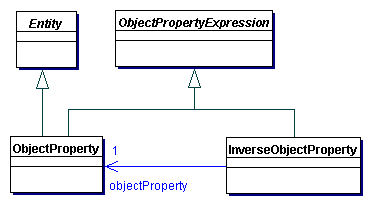
\includegraphics[width=120mm]{Figures/object_property_expression.png}
	\caption{Mô tả thuộc tính đối tượng OWL 2\label{overflow}}
\end{figure}
Như được thể hiện trong hình, OWL 2 hỗ trợ 2 loại mô tả thuộc tính đối tượng. Thuộc tính đối tượng là dạng đơn giản của mô tả thuộc tính đối tượng, thuộc tính đối tượng nghịch đảo (inverse object properties) cho phép thể hiện các mối quan hệ 2 chiều giữa biểu hiện các mô tả lớp (class expression) và các phát biểu (axiom).
\\ \textbf{Mô tả thuộc tính đối tượng nghịch đảo}

\begin{verbatim}
ObjectPropertyAssertion( a:fatherOf a:Peter a:Steve) 
// Peter là ba của Steve
\end{verbatim}}
Với phát biểu trên, ontology sẽ hiểu \textit{a:Steve} liên kết với \textit{a:Peter} qua một thuộc tính nghịch đảo của \textit{a:fatherOf} là \textit{ObjectInverseOf( a:fatherOf)}. Chúng ta cũng có thể khai báo tường minh nghịch đảo của \textit{a:fatherOf} là \textit{a:childOf} bằng phát biểu  \textit{InverseObjectProperties( a:fatherOf a:childOf )}.

% Data Property Expression
\paragraph{Mô tả thuộc tính dữ liệu (Data Property Expression)}
Tương đương với biểu hiện thuộc tính đối tượng, trong tài liệu cấu trúc chi tiết của OWL2 cũng giới thiệu định nghĩa mô tả thuộc tính dữ liệu (data property expressions), nhằm biểu diễn mối quan hệ giữa một cá thể và một trực nghĩa. Cấu trúc của mô tả thuộc tính dữ liệu thể hiện trong hình bên. Như chúng ta thấy thuộc tính dữ liệu (data property) cũng chính là 1 mô tả thuộc tính dữ liệu (data property expression), cấu trúc như vậy được xây dựng nhằm tạo thuận lợi cho nhu cầu mở rộng sau này nếu có.
\begin{figure}[h!]
	\centering
	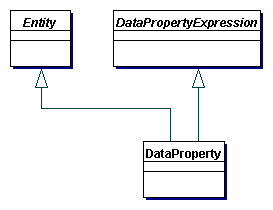
\includegraphics[width=110mm]{Figures/data_property_expression.png}
	\caption{Cấu trúc của mô tả thuộc tính dữ liệu OWL 2\label{overflow}}
\end{figure}

%Data ranges
\subsubsection{Miền dữ liệu (Data Range)}
Kiểu dữ liệu như \textit{xsd:string} hoặc \textit{xsd:integer} và trực nghĩa \verb|"1"^^xsd:integer| được dùng để biểu diễn miền dữ liệu - tập hợp danh sách có thứ tự (tuples) của các trực nghĩa, mà mỗi phần tử trong danh sách này chỉ chứa một trực nghĩa duy nhất để định nghĩa chính nó. Miền dữ liệu được dùng để tạo ra ràng buộc (hay những dữ liệu hợp lệ) cho thuộc tính dữ liệu. Cấu trúc của miền dữ liệu trong OWL 2 được mô tả trong hình. Thành phần đơn giản của miền dữ liệu chính là kiểu dữ liệu : một kiểu dữ liệu (Datatype) cũng chính là một miền dữ liệu (Data Range).
\begin{figure}[h!]
	\centering
	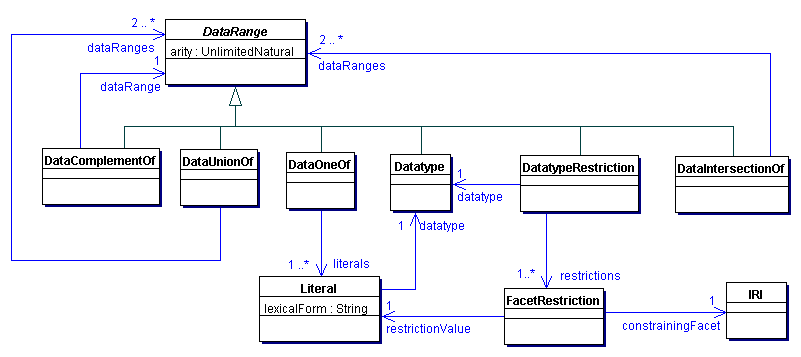
\includegraphics[width=150mm, height=80mm]{Figures/datarange.png}
	\caption{Cấu trúc miền dữ liệu (data range) quy định theo OWL 2\label{overflow}}
\end{figure}

% DataIntersectionOf
\paragraph{Giao của các miền dữ liệu (Intersection of Data Ranges)}
Giao của miền dữ liệu \textit{DataIntersectionOf(} $DR_{1} ... DR_{n}$ \textit{)}  chứa tất cả các danh sách của các trực nghĩa nằng trong $DR_{i}$ với $1 <= i <= n$. Tất cả miền dữ liệu $DR_{i}$ phải có cùng số lượng tham số, và cũng phải có cùng số lượng số kết quả trả về. Ví dụ về miền dữ liệu chỉ chứa số 0:
\begin{verbatim}
DataIntersectionOf( xsd:nonNegativeInteger xsd:nonPositiveInteger )
\end{verbatim}

% DataUnionOf
\paragraph{Hội của các miền dữ liệu (Union of Data Ranges)}
Điều kiện về số lượng tham số và số lượng kết quả trả về của từng $DR_{i}$ với điều kiện $1 <= i <= n$ phải giống nhau. Cú pháp \textit{DataIntersectionOf( $DR_{1} ... DR_{n}$ )}. Ví dụ về việc miền dữ liệu chứa tất cả các chuỗi và số nguyên:
\begin{verbatim}
DataUnionOf( xsd:string xsd:integer )
\end{verbatim}

% DataComplementOf
\paragraph{Phủ định của miền dữ liệu (Complement of Data Ranges)}
Cú pháp \textit{DataComplementOf( DR )} chứa tất cả các miền dữ liệu còn lại trong miền dữ liệu \textit{DR}. Yêu câu số lượng tham số và kết quả phải bằng \textit{DR}
\begin{verbatim}
DataComplementOf( xsd:positiveInteger )
\end{verbatim}
\textbf{Giải thích:} miền dữ liệu trên chứa tất cả số nguyên âm, số 0; và chứa tất cả chuỗi (strings) vì chuỗi không phải số nguyên dương.

% DataOneOf
\paragraph{Liệt kê trực nghĩa (Enumeration Of Literals)}
Một danh sách liệt kê các trực nghĩa (literals) với cú pháp \textit{DataOneOf(} $lt_{1} ... lt_{n}$ \textit{)},  $lt_{i}$ với $1 <= i <= n$.  Miền dữ liệu chỉ áp dụng lên một trực nghĩa nằm trong danh sách (\textit{"oneOf"}). Ví dụ khai báo miền dữ liệu cho thuộc tính dữ liệu \textit{canMoveOnOrIn} chỉ có thể là một trong 4 giá trị chuỗi \textit{"OnRoadOrOffRoad"}, \textit{"Rail"}, \textit{"Sky"} và \textit{"Water"}.
\begin{verbatim}
DataPropertyRange(:canMoveOnOrIn 
DataOneOf("OnRoadOrOffRoad" "Rail" "Sky" "Water"))
\end{verbatim}

% Datatype Restrictions
\paragraph{Ràng buộc cho kiểu dữ liệu (Datatype Restrictions)}
Một ràng buộc cho kiểu dữ liệu (hay một tập các giá trị hợp lệ của kiễu dữ liệu) \textit{DatatypeRestriction(} $DT$ $F_{1}$ $lt_{1}$ ... $F_{n}$ $lt_{n}$ \textit{ )} gồm một kiểu dữ liệu đơn (unary datatype) $DT$ và $n$ cặp $($ $F_{i}$, $lt_{i}$ $)$. Vùng dữ liệu hợp lệ được tính ra bằng cách hạn chế vùng giá trị của $DT$ và lấy giao tất cả các cặp $(F_{i}$, $v_{i}$ $)$ trong đó $v_{i}$ là giá trị dữ liệu của trực nghĩa $lt_{i}$. Ví dụ miền dữ liệu sau chỉ gồm đúng các số 5,6,7,8,9:
\begin{verbatim}
DatatypeRestriction( xsd:integer 
xsd:minInclusive "5"^^xsd:integer xsd:maxExclusive "10"^^xsd:integer )
\end{verbatim}

% Class Expressions
\subsubsection{Mô tả lớp (Class Expression)}
Trong OWL2, các lớp và mô tả thuộc tính (property expressions) được sử dụng để xây dựng nên các mô tả lớp, hay chúng được gọi là các miêu tả hoặc trong thuật ngữ của Description Logic chúng được gọi là \textit{những khái niệm phức tạp}. Các mô tả lớp 
biểu diễn tập hợp các cá thể bằng cách chính thức đặt ra các điều kiện quy định cho các thuộc tính của các cá thể này; cá thể nào có những thuộc tính phù hợp hay thỏa những quy định đó được xem là một thành viên của mô tả lớp đang xét. Có 5 dạng mô tả lớp chính. Sau đây chúng em xin được trình bày 3 dạng mô tả lớp.
% Propositional Connectives and Enumeration of Individuals
\paragraph{Các mệnh đề logic và liệt kê cá thể}
\begin{figure}[h]
	\centering
	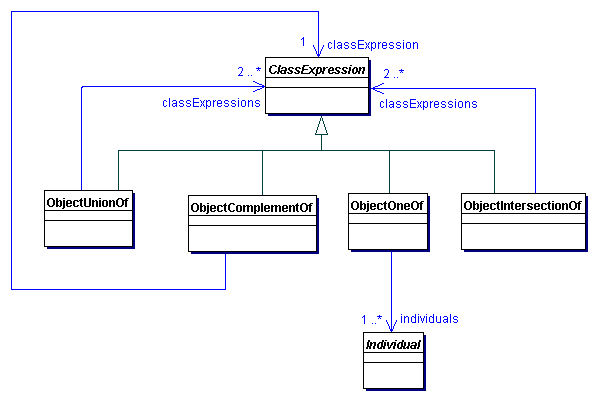
\includegraphics[width=150mm]{Figures/ce_0.png}
	\caption{Mô tả lớp trong OWL 2\label{overflow}}
\end{figure}
OWL2 cho phép liệt kê các cá thể của một lớp, khai báo các mệnh đề logic như trong hình sau. Các khai báo \textit{ObjectIntersectionOf}, \textit{ObjectUnionOf}, và \textit{ObjectComplementOf} cho phép thực hiện các phép toán luận lý (and ,or, not) trên những mô tả lớp. \textit{ObjectOneOf} quy định chính xác những cá thể cho mô tả lớp đang khai báo.

%% Intersection of Class Expressions\subparagraph{Intersection of Class Expressions} Tập giao của các mô tả lớp \textit{ObjectIntersectionOf(} $CE_{1}$ ... $CE_{n}$ \textit{)} gồm tất cả các cá thể là thành viên của tất cả các mô tả lớp $CE_{i}$ với $1<=i<=n$. Ví dụ: 
\begin{verbatim}
ClassAssertion(a:Engineer a:Peter)  // Peter là kĩ sư.
ClassAssertion(a:Teacher a:Peter) // Peter là giáo viên.
\end{verbatim}
\textbf{Giải thích: } với khai báo như trên, một hàm ý sẽ được suy ra mà không cần khai báo đó là \textit{Peter vừa là giáo viên vừa là kĩ sư} hay tương đương với phát biểu \textit{ObjectIntersectionOf( a:Engineer a:Teacher )}. 

%% Union of Class Expressions
\subparagraph{Union of Class Expressions} Tập hội của lớp \textit{ObjectUnionOf(} $CE_{1}$ ... $CE_{n}$ \textit{)} chức tất cả các cá thể là thành viên của của ít nhất một mô tả lớp $CE_{i}$ với $1<=i<=n$. Ví dụ:
\begin{verbatim}
ClassAssertion( a:Man a:Peter )	 // Peter là nam
ClassAssertion( a:Woman a:Lois ) // Lois là nữ
\end{verbatim}
\textbf{Giải thích: } với khai báo như trên, một hàm ý sẽ được suy ra mà không cần khai báo đó là \textit{cả Peter và Lois đều thuộc lớp nam hoặc nữ} hay tương đương với phát biểu O\textit{bjectUnionOf( a:Man a:Woman )}.

%% Complement of Class Expressions
\subparagraph{Complement of Class Expressions} Phủ định của một mô tả lớp chứa tất cả các phần tử không thuộc mô tả lớp đó. Cú pháp \textit{ObjectComplementOf(CE)}. Ví dụ:
\begin{verbatim}
DisjointClasses( a:Man a:Woman) 
// Không có cá thể nào vừa làm nam vừa là nữ
ClassAssertion( a:Woman a:Lois) 
// Lois là nữ
\end{verbatim}
\textbf{Giải thích:} Vì \textit{Lois} là nữ và không có cá thể nào vừa là nam vừa là nữ nên \textit{Lois} thuộc lớp \textit{không phải nam} tương đương với phát biểu \textit{ObjectComplementOf( a:Man )}.

\subparagraph{Enumeration of Individuals} Liệt kê các cá thể \textit{ObjectOneOf(} $a_{1}$ ... $a_{n}$ \textit{)} chứa duy nhất một cá thể $a_{i}$ với $1<=i<=n$. 

% Object Property Restrictions 
\paragraph{Ràng buộc theo thuộc tính đối tượng (Object Property Restrictions)}
\begin{figure}[h]
	\centering
	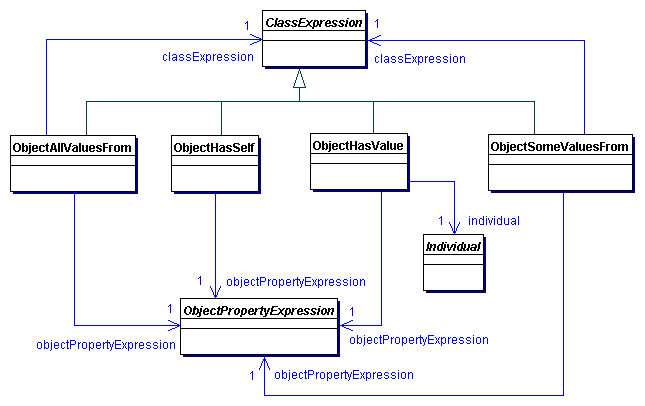
\includegraphics[width=150mm]{Figures/ce_1.png}
	\caption{Object Property Restrictions trong OWL 2\label{overflow}}
\end{figure}
Các mô tả lớp trong OWL 2 có thể được tạo ra bằng cách kết hợp chúng với các thuộc tính đối tượng bằng phát biểu như trong hình.
\paragraph{Existential Quantification} Một mô tả lớp \textit{ObjectSomeValueFrom( OPE CE )} thể hiện mối quan hệ giữa những cá thể được kết nối bởi mô tả thuộc tính đối tượng \textit{OPE} đến \textbf{ít nhất một} cá thể thuộc mô tả lớp \textit{CE}. Ví dụ:
\begin{verbatim}
ObjectPropertyAssertion( a:fatherOf a:Peter a:Steve ) 
// Peter là ba của Steve                    
ClassAssertion( a:Kid a:Steve )         
// Steve là trẻ con.
\end{verbatim} 
\textbf{Giải thích:} với khai báo như trên, một hàm ý sẽ được suy ra mà không cần khai báo đó là \textit{Peter là ba của một vài (ít nhất một) đứa trẻ} hay tương đương với phát biểu \textit{ObjectSomeValuesFrom( a:fatherOf a:Kid )}.

\subparagraph{Universal Quantification} Mô tả lớp \textit{ObjectAllValuesFrom( OPE CE)} thể hiện mối quan hệ giữa những cá thể được kết nối bởi mô tả thuộc tính đối tượng $OPE$ đến \textbf{tất cả} các cá thể thuộc mô tả lớp $CE$. Ví dụ: 
\begin{verbatim}
ObjectPropertyAssertion( a:hasPet a:Peter a:Tom)
// Tom là vật nuôi của Peter
ClassAssertion( a:Cat a:Tom) 
// Tom là một con mèo
ClassAssertion( ObjectMaxCardinality( 1 a:hasPet ) a:Peter )
// Peter chỉ được phép có một vật nuôi
\end{verbatim}
\textbf{Giải thích:} với khai báo như trên, một hàm ý sẽ được suy ra mà không cần khai báo đó là \textit{Peter thuộc mô tả lớp "có tất cả vật nuôi là mèo"} hay tương đương với phát biểu \textit{ObjectAllValuesFrom( a:hasPet a:Cat )}.

\subparagraph{Individual Value Restriction} Mô tả  \textit{ObjectHasValue(OPE a)} thể hiện mối quan hệ giữa tất cả các cá thể được kết nối bởi mô tả thuộc tính đối tượng \textit{OPE} và cá thể $a$. Ví dụ:
\begin{verbatim}
ObjectPropertyAssertion( a:fatherOf a:Peter a:Steve)
// Peter là ba của Steve
\end{verbatim}
\textbf{Giải thích:} với khai báo như trên, \textit{Peter thuộc mô tả lớp sau} mà không cần khai báo là \textit{ObjectHasValue( a:fatherOf a:Steve )}.

\subparagraph{Self-Restriction} Mô tả \textit{ObjectHasSelf( OPE )} thể hiện mối quan hệ giữa tất cả các cá thể được kết nối bởi mô tả thuộc tính đối tượng \textit{OPE} với chính chúng. Ví dụ:
\begin{verbatim}
ObjectPropertyAssertion( a:quayQuanhTruc a:TraiDat a:TraiDat )	
// Trái đất quay quanh trục của trái đất.
\end{verbatim}
\textbf{Giải thích:} với khai báo như trên, \textit{a:TraiDat thuộc mô tả lớp sau} mà không cần khai báo là \textit{ObjectHasSelf( a:quayQuanhTruc )}.

% Object Property Cardinality Restrictions
\paragraph{Ràng buộc thuộc tính đối tượng theo số lượng}
\begin{figure}[h]
	\centering
	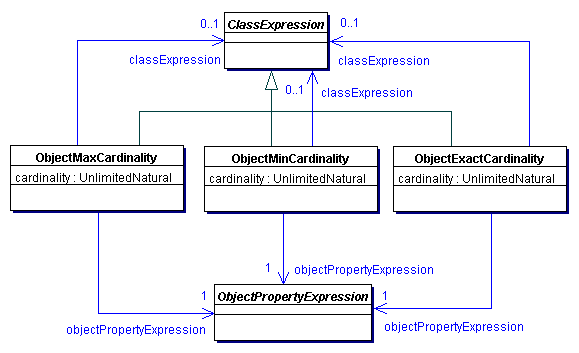
\includegraphics[width=150mm]{Figures/ce_2.png}
	\caption{Object Property Cardinality Restrictions trong OWL 2\label{overflow}}
\end{figure}
Các mô tả lớp trong OWL 2 có thể được tạo ra bằng cách đặt ra những số lượng hạn chế các cá thể mà các thuộc tính đối tượng có thể liên kết.
\subparagraph{Số lượng tối thiểu (Minimum Cardinality)} - mô tả \textit{ObjectMinCardinality(n OPE  CE)} biểu diễn mọi các thể được kết nối bởi mô tả thuộc tính đối tượng \textit{OPE} đến số lượng tối thiểu $n$ cá thể (khác nhau) thuộc mô tả lớp \textit{CE} với $n$ là số nguyên không âm. Nếu \textit{CE} không được khai báo trong phát biểu trên mặc định sẽ là $owl:Thing$. Ví dụ:
\begin{verbatim}
ObjectPropertyAssertion( a:fatherOf a:Peter a:Steve )
ObjectPropertyAssertion( a:fatherOf a:Peter a:Bush )
ClassAssertion( a:Kid a:Steve )
ClassAssertion( a:Kid a:Bush )
\end{verbatim}
\textbf{Giải thích:} với các điều kiện như trên thì Peter sẽ được ngầm hiểu thành viên của mô tả lớp sau 
$ObjectMinCardinality($ 2 a:fatherOf a:Kid $)$ - Peter là bố của ít nhất 2 đứa trẻ.

\subparagraph{Số lượng tối đa (Maximum Cardinality)} Mô tả \textit{ObjectMaxCardinality( n OPE CE)} biểu diễn mọi các thể được kết nối bởi mô tả thuộc tính đối tượng $OPE$ đến số lượng tối đa $n$ cá thể (khác nhau) thuộc mô tả lớp \textit{CE} với $n$ là số nguyên không âm. Nếu $CE$ không được khai báo trong phát biểu trên mặc định sẽ là \textit{owl:Thing}. Ví dụ:
\begin{verbatim}
ObjectPropertyAssertion( a:hasPet a:Peter a:Tom)
// Peter có vật nuôi là Tom
ClassAssertion( ObjectMaxCardinality( 1 a:hasPet ) a:Peter )
// Peter thuộc lớp "những ai có tối đa 1 vật nuôi"
\end{verbatim}
\textbf{Giải thích:} theo 2 điều kiệu trên thì Peter sẽ thuộc mô tả lớp \textit{ObjectMaxCardinality( 2 a:hasPet )} chỉ những "ai có tối đa 2 vật nuôi" (số vật nuôi <= 2), vì 2 phát biểu đầu tiên chỉ ra rằng Peter chắc chắn chỉ có một vật nuôi.

\subparagraph{Số lượng chính xác (Exact Cardinality)} - mô tả \textit{ObjectExactCardinality( n OPE CE)} biểu diễn mọi các thể được kết nối bởi mô tả thuộc tính đối tượng \textit{OPE} đến số lượng chính xác $n$ cá thể (khác nhau) thuộc mô tả lớp $CE$ với $n$ là số nguyên không âm. Nếu \textit{CE} không được khai báo trong phát biểu trên mặc định sẽ là \textit{owl:Thing}. Mô tả lớp này tương được khi lấy giao của 2 mô tả số lượng tối đa và số lượng tối thiểu cùng $n$.
\begin{verbatim}
ObjectIntersectionOf( ObjectMinCardinality( n OPE CE ) 
ObjectMaxCardinality( n OPE CE ) ).
\end{verbatim}

% Data Property Restrictions
\paragraph{Ràng buộc theo thuộc tính dữ liệu (Data Property Restrictions)}
\begin{figure}[h]
	\centering
	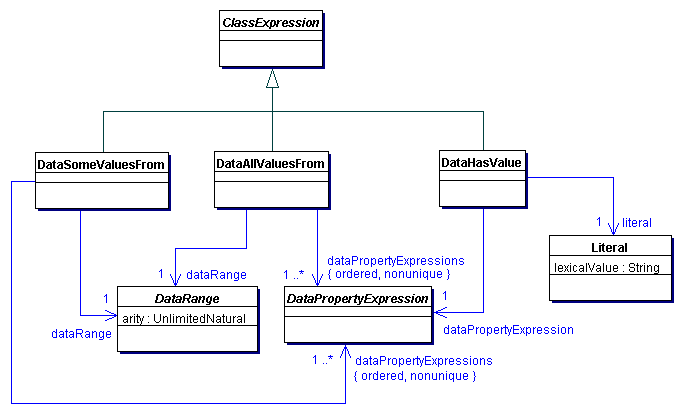
\includegraphics[width=150mm]{Figures/ce_3.png}
	\caption{Data Property Restrictions trong OWL 2\label{overflow}}
\end{figure}
Mô tả lớp dạng này được tạo ra bằng cách đặc các ràng buộc về kiểu dữ liệu, giới hạn các giá trị dữ liệu lên mô tả thuộc tính dữ liệu (data property expression) như trong hình. Những mô tả này cũng tương tự như ràng buộc thuộc tính đối tượng vừa nêu ra ở trên.

%% Existential Quantification
\subparagraph{Existential Quantification} Một mô tả lớp \textit{DataSomeValuesFrom(} $DPE_{1}$ ... $DPE_{n}$ $DR$ \textit{)} gồm $n$ mô tả thuộc tính dữ liệu $DPE_{i}$, $1<=i<=n$, và một miền dữ liệu (data range) $DR$ với số lượng tham số phải bằng $n$. Mô tả lớp này biểu diễn mối quan hệ dữ liệu giữa tất cả các cá thể kết nối với $DPE_{i}$ tới các trực nghĩa $lt_{i}$, $1<=i<=n$ với $($ $lt_{1}$ ... $lt_{n}$ $)$ trong $DR$. Ví dụ:
\begin{verbatim}
DataPropertyAssertion( a:hasAge a:Steve "17"^^xsd:integer ) // Steve 17 tuổi.
\end{verbatim}
\textbf{Giải thích:} Vì Steve 17 tuổi nên chúng ta ngầm hiểu rằng Steve thuộc những ai có số tuổi là số nguyên và không lớn hơn 20 tuổi, tương đương phát biểu sau
\begin{verbatim}
DataSomeValuesFrom( a:hasAge 
DatatypeRestriction( xsd:integer xsd:maxExclusive "20"^^xsd:integer ) )
\end{verbatim}

%% Universal Quantification
\subparagraph{Universal Quantification} Một mô tả lớp \textit{DataAllValuesFrom(} $DPE_{1}$ ... $DPE_{n}$ $DR$ \textit{)} gồm $n$ mô tả thuộc tính dữ liệu $DPE_{i}$, $1<=i<=n$, và một miền dữ liệu (data range) $DR$ với số lượng tham số phải bằng $n$. Mô tả lớp này biểu diễn mối quan hệ dữ liệu giữa tất cả các cá thể \textbf{chỉ} \textit{(only)} kết nối với $DPE_{i}$ tới các trực nghĩa $lt_{i}$, $1<=i<=n$ với $($ $lt_{1}$ ... $lt_{n}$ $)$ trong $DR$. Ví dụ: 
\begin{verbatim}
DataPropertyAssertion( a:hasZIP _:a1 "70000"^^xsd:integer ) 
// Mã vùng của _:a1 là số nguyên 70000
FunctionalDataProperty( a:hasZIP) 
// Mỗi đối tượng chỉ có duy nhất một mã vùng
\end{verbatim}
\textbf{Giải thích:} Mã vùng của một số quốc gia như Anh và Canada là dạng chuỗi (chứa ký tự và số), dựa vào 2 phát biểu trên chúng ta có thể hiểu rằng mã vùng của \verb|_a:1| thuộc mô tả những mã vùng \textbf{chỉ} gồm số nguyên $DataAllValuesFrom( a:hasZIP xsd:integer )$

% Literal Value Restriction
\subparagraph{Ràng buộc bằng giá trị trực nghĩa - Literal Value Restriction}
Một mô tả \textit{DataHasValue(} $DPE$ $lt$ \textit{)} gồm một mô tả thuộc tính dữ liệu \textit{DPE} và một trực nghĩa $lt$, nó biểu diễn quan hệ của những cá thể nào qua \textit{DPE} tới $lt$. Ví dụ:
\begin{verbatim}
DataPropertyAssertion( a:hasAge a:Steve "17"^^xsd:integer )
\end{verbatim}
\textbf{Giải thích:} Steve là thành viên của mô tả lớp sau mà không cần khai báo "những ai 17 tuổi".
\begin{verbatim}
DataHasValue( a:hasAge "17"^^xsd:integer )
\end{verbatim}

% Data Property Cardinality Restrictions
\paragraph{Ràng buộc thuộc tính dữ liệu theo số lượng}
\begin{figure}[h]
	\centering
	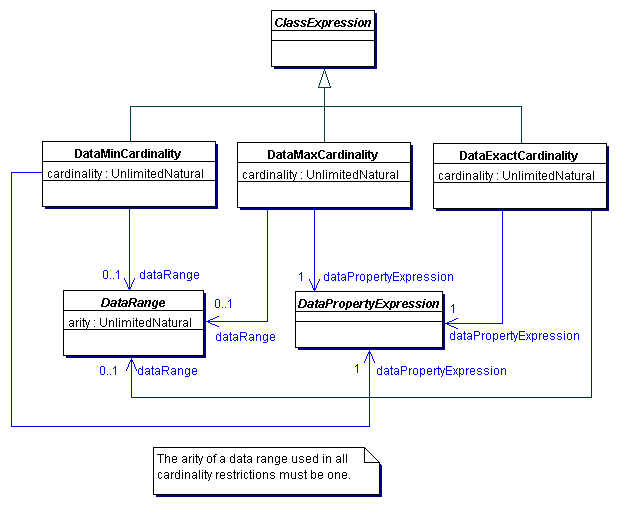
\includegraphics[width=150mm]{Figures/ce_4.png}
	\caption{Data Property Cardinality Restrictions trong OWL 2\label{overflow}}
\end{figure}
Tương tự ràng buộc thuộc tính đối tượng theo số lượng, OWL 2 cũng cho phép chúng ta tạo ra các mô tả lớp bằng cách các giá trị dữ liệu ( thay vì cá thể) mà thuộc tính dữ liệu có thể liên kết đến. Cấu trúc được mô tả như trong hình.

%% Minimum Cardinality)
\subparagraph{Số lượng tối thiểu (Minimum Cardinality)} Một mô tả lớp \textit{DataMinCardinality( n DPE DR)}  biểu diễn mọi cá thể được kết nối bởi thuộc tính dữ liệu \textit{DPE} đến số lượng tối thiểu $n$ các trực nghĩa khác nhau thuộc miền dữ liệu  \textit{DR} với $n$ số nguyên không âm. Nếu \textit{DR} không được khai báo trong phát biểu trên mặc định sẽ là \textit{rdfs:Literal}. Ví dụ:
\begin{verbatim}
DataPropertyAssertion( a:hasPhoneNumber a:Steve "0123456789" )
DataPropertyAssertion( a:hasPhoneNumber a:Steve "0987654321" )
\end{verbatim}
\textbf{Giải thích:} Với 2 phát biểu như trên tồn tại, có thể hiểu Steve thuộc lớp những ai có ít nhất 2 số điện thoại \textit{DataMinCardinality(2 a:hasPhoneNumber)}.

%% Maximum Cardinality
\subparagraph{Số lượng tối đa (Maximum Cardinality)} Một mô tả lớp \textit{DataMaxCardinality( n DPE DR)} biểu diễn mọi cá thể được kết nối bởi thuộc tính dữ liệu $DPE$ đến số lượng tối đa $n$ các trực nghĩa khác nhau thuộc miền dữ liệu  $DR$ với $n$ số nguyên không âm. Nếu $DR$ không được khai báo trong phát biểu trên mặc định sẽ là $rdfs:Literal$. Ví dụ:
\begin{verbatim}
DataPropertyAssertion( a:hasID a:Steve "0001" ) // Steve số CMND là 0001
FunctionalDataProperty( a:hasID ) // Mỗi người chỉ có duy nhất một số CMND
\end{verbatim}
\textbf{Giải thích:} Với 2 phát biểu như trên tồn tại, có thể hiểu Steve thuộc lớp "những ai có nhiều nhất 2 số CMND" ( số CMND <=2), \textit{DataMaxCardinality(2 a:hasID)}.

%% Exact Cardinality
\subparagraph{Số lượng chính xác (Exact Cardinality)} Một mô tả lớp \textit{DataExactCardinality( n DPE DR)}  biểu diễn mọi cá thể được kết nối bởi thuộc tính dữ liệu \textit{DPE} đến số lượng chính xác $n$ các trực nghĩa khác nhau thuộc miền dữ liệu  \textit{DR} với $n$ số nguyên không âm. Nếu \textit{DR} không được khai báo trong phát biểu trên mặc định sẽ là \textit{rdfs:Literal}. Ví dụ:
\begin{verbatim}
DataPropertyAssertion( a:hasID a:Steve "0001" ) // Steve số CMND là 0001
FunctionalDataProperty( a:hasID ) // Mỗi người chỉ có duy nhất một số CMND
\end{verbatim}
\textbf{Giải thích:} Với 2 phát biểu như trên tồn tại, có thể hiểu Steve thuộc lớp "có duy nhất 1 CMND" \textit{DataExactCardinality(1 a:hasName)}.

% Axioms
\subsubsection{Các tiên đề (Axioms)}
{\let\thefootnote\relax\footnotetext{* Lưu ý:\textit{
			Trong nội dung báo cáo này chúng em sẽ gọi vắng tắt các tiên đề - những phát biểu hiển nhiên đúng trong một lĩnh vực là \textit{những phát biểu} nhằm diễn giải các lý thuyết, nguyên lý trở dễ hiểu hơn.
		}}
	}
	Thành phần chính của một OWL 2 Ontology chính là một tập hợp gồm các tiên đề \textsuperscript{*} - những phát biểu mà chúng ta cho là đúng trong một lĩnh vực. OWL 2 cung cấp một loạt các loại phát biểu được mở rộng (thừa kế) từ lớp \textbf{Axiom} như trong hình. Các phát biểu có thể là các phát biểu khai báo (declarations), phát biểu về lớp, phát biểu về thuộc tính đối tượng/dữ liệu, phát biểu định nghĩa kiểu dữ liệu, khóa (HasKey), phát biểu khẳng định (assertions), và các phát biểu chú thích (annotations). Có thể nói những phát biểu (tiên đề) chính là những viên gạch để chúng ta xây dựng nên các tầng ngữ nghĩa (semantic) cho ontology.
	\begin{figure}[!h]
		\centering
		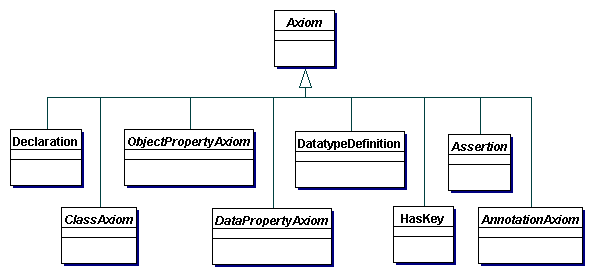
\includegraphics[width=150mm]{Figures/axioms.png}
		\caption{Các dạng phát biểu của OWL 2\label{overflow}}
	\end{figure}
	
	\paragraph{Phát biểu về mô tả lớp - Class Expression Axioms}
	Những phát biểu này cho phép biểu diễn các loại quan hệ giữa những mô tả lớp (Class Expressions) với nhau. Có 4 phát biểu được mở rộng ra từ phát biểu này như trong hình.
	\begin{figure}[!h]
		\centering
		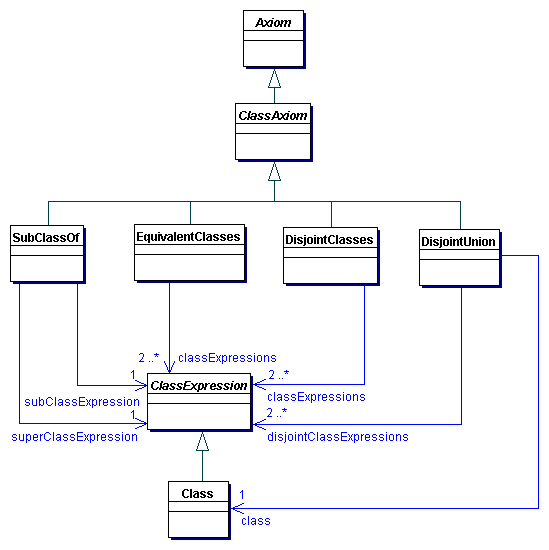
\includegraphics[width=120mm]{Figures/classAxiom.png}
		\caption{Các dạng phát biểu về lớp của OWL 2\label{overflow}}
	\end{figure}
	
	\subparagraph{Phát biểu lớp con (SubClass Axioms)} - một phát biểu \textit{SubClassOf(}$CE_{1}$ $CE_{2}$ \textit{)} nói rằng mô tả lớp $CE_{1}$ là lớp con của mô tả lớp $CE_{2}$. Phát biểu này là phát biểu cơ bản trong OWL 2 được sử dụng để xây dựng một phân cấp lớp trong Ontology. Ví dụ:
	\begin{verbatim}
	SubClassOf( a:Driver a:Adult ) // Mỗi tài xế là một người trưởng thành.
	SubClassOf( a:Adult a:Person ) // Mỗi người trưởng thành là một người.
	ClassAssertion (a:Driver a:Steve ) // Steve là một tài xế.
	\end{verbatim}
	\textbf{Giải thích:} nhờ 2 phát biểu đầu tiên, chúng ta ngầm hiểu tài xế cũng là một người trưởng thành, cũng là một người, vì vậy tất cả những cá thể là tài xế, cũng là người trưởng thành và cũng là người -> Steve là cũng là thành viên của 2 lớp $Adult$ và $Person$.
	
	\subparagraph{Phát biểu lớp tương đương (Equivalent Classes)} - một phát biểu \textit{EquivalentClasses( $CE_{1}$ $CE_{n}$ )} nói rằng mỗi mô tả lớp $CE_{i}$, $1<=i<=n$ đều đồng nghĩa với các tất cả các mô tả lớp còn lại trong phát biểu này. Phát biểu \textit{EquivalentClasses( $CE_{2}$ $CE_{1}$ )} tương đương \textit{EquivalentClasses( $CE_{1}$ $CE_{2}$ )}. Ví dụ:
	\begin{verbatim}
	EquivalentClasses( a:Bike  a:Bicycle )
	\end{verbatim}
	
	\subparagraph{Disjoint Classes} - một phát biểu \textit{DisjointClasses( $CE_{1}$ ... $CE_{n}$ )} nói rằng không cá thể nào của $CE_{i}$ thuộc $CE_{j}$ và ngược lại với $i \neq j$, $1<=i,j<=n$. Ví dụ:
	\begin{verbatim}
	DisjointClasses( a:Man a:Woman )	
	ClassAssertion( a:Man a:Steve )
	\end{verbatim}
	\textbf{Giải thích:} Steve không là nữ - \textit{ObjectComplementOf( a:Girl )}, nếu chúng ta khai báo thêm $ClassAssertion($ $a:Girl$ $a:Steve)$ sẽ làm cho ontology bị thiếu tính nhất quán (sẽ được nếu rõ hơn ở các chương sau).
	
	\paragraph{Phát biểu về thuộc tính đối tượng (Object Property Axioms)}
	Những phát biểu này cho phép biểu diễn các loại quan hệ giữa những mô tả thuộc tính đối tượng (Object Property Expressions) với nhau.
	\begin{figure}[h]
		\centering
		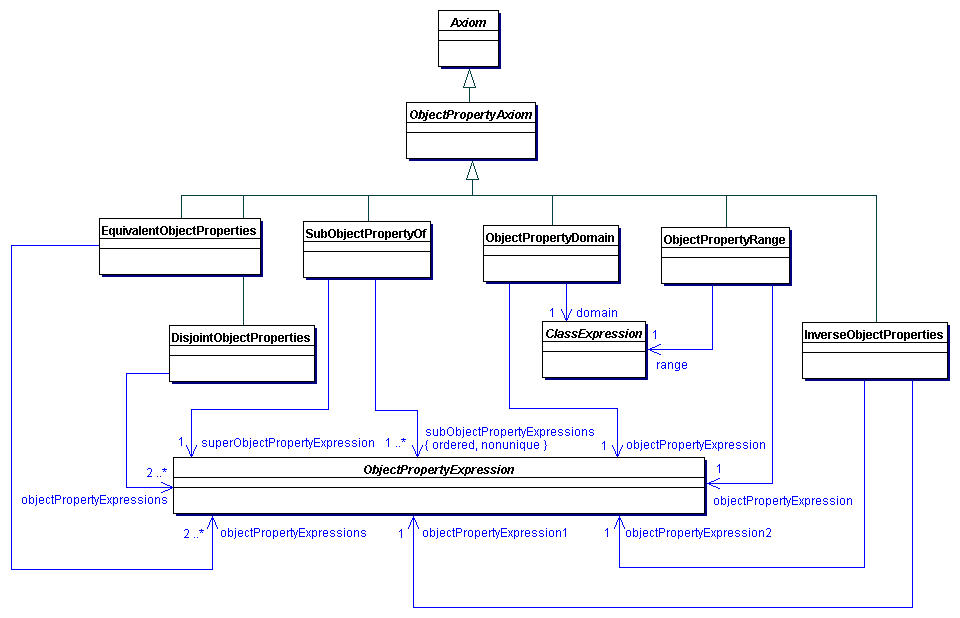
\includegraphics[width=160mm]{Figures/objectpropertyAxiom.png}
		\caption{Các dạng phát biểu về thuộc tính đối tượng của OWL 2 (phần 1)\label{overflow}}
	\end{figure}
	
	\subparagraph{Thuộc tính đối tượng con (SubObjectPropertyOf)} - một phát biểu \textit{SubObjectPropertyOf( $OPE_{1}$ $OPE_{2}$ )} nói rằng mô tả thuộc tính đối tượng $OPE_{1}$ là thuộc tính con của mô tả thuộc tính đối tượng $OPE_{2}$, có nghĩa nếu một cá thể $x$ được liên kết bởi $OPE_{1}$ với $y$ thì $x$ cũng được liên kết bởi $OPE_{2}$ đến $y$. Ví dụ:
	\begin{verbatim}
	SubObjectPropertyOf( a:hasCat a:hasPet )     
	ObjectPropertyAssertion( a:hasCat a:Peter a:Tom) // Peter có con mèo là Tom
	\end{verbatim}
	\textbf{Giải thích:} Ai có mèo thì cũng có thể hiểu là người đó có vật nuôi theo phát biểu đầu tiên, dựa theo phát biểu thứ hai chúng ta có ngầm hiểu là \textit{Peter có vật nuôi là Tom} - \textit{ObjectPropertyAssertion( a:hasPet a:Peter a:Tom )}.
	
	\subparagraph{Thuộc tính đối tượng tương đương (Equivalent Object Properties)} - một phát biểu \textit{EquivalentObjectProperties( $OPE_{1}$ ... $OPE_{n}$ )} nói rằng mỗi mô tả thuộc tính $OPE_{i}$, $1<=i<=n$ đều đồng nghĩa với các tất cả các mô tả thuộc tính còn lại trong phát biểu này phát biểu \textit{EquivalentObjectProperties( $OPE_{2}$ $OPE_{1}$ )} tương đương \textit{EquivalentObjectProperties( $OPE_{1}$ $OPE_{2}$ )}. Ví dụ:
	\begin{verbatim}
	EquivalentObjectProperties( a:hasBrother a:hasMaleSibling ) 
	ObjectPropertyAssertion( a:hasBrother a:Chris a:Steve )     
	// Steve là anh của Chris
	ObjectPropertyAssertion( a:hasMaleSibling a:Steve a:Chris ) 
	// Chris là anh chị em ruột (mà là nam) của Steve
	\end{verbatim}
	\textbf{Giải thích:} Do phát biểu đầu tiên có nghĩa "có anh" đồng nghĩa với "có anh chị em ruột (là nam)", từ 2 phát biểu sau chúng ta có thể suy ra các phát biểu sau mà cần khai báo chúng \textit{ObjectPropertyAssertion(a:hasMaleSibling a:Chris a:Steve)} và \textit{ObjectPropertyAssertion(a:hasBrother a:Stewie a:Chris)}.
	
	\subparagraph{Disjoint Object Properties} - một phát biểu \textit{DisjointObjectProperties($OPE_{1}$ ... $OPE_{n}$)} nói rằng không cá thể được liên kết bởi cả của $OPE_{i}$ và $OPE_{j}$ với $i \neq j$, $1<=i,j<=n$. Ví dụ:
	\begin{verbatim}
	DisjointObjectProperties( a:hasFather a:hasMother ) Có ba khác có mẹ.
	ObjectPropertyAssertion( a:hasFather a:Steve a:Peter )	Peter là ba của Steve.
	ObjectPropertyAssertion( a:hasMother a:Steve a:Lois ) Lois là mẹ của Steve.
	\end{verbatim}
	Nếu thêm phát biểu \textit{ObjectPropertyAssertion(a:hasMother a:Steve a:Peter)} sẽ dẫn đến tính thiếu nhất quán.
	
	\subparagraph{Thuộc tính đối tượng nghịch đảo} - \textit{phát biểu InverseObjectProperties( $OPE_{1}$ $OPE_{2}$ )} nói rằng thuộc tính đối tượng $OPE_{2}$ là nghịch đảo của $OPE_{1}$. Nếu cá thể $x$ được kết nối bởi $OPE_{1}$ tới cá thể $y$, thì $y$ sẽ được kết nối bởi $OPE_{2}$ tới $x$ và ngược lại. Ví dụ:
	\begin{verbatim}
	InverseObjectProperties( a:parentOf a:childOf )
	ObjectPropertyAssertion( a:childOf a:Peter a:Steve ) 
	// Steve là con của Peter
	\end{verbatim}
	\textbf{Giải thích:} Phát biểu đầu có thể hiểu "nếu x là con y" thì "y là ba mẹ của x", do vậy từ các phát biểu trên ta suy ra được Peter là ba mẹ của Steve tương đương \textit{ObjectPropertyAssertion( a:parentOf a:Steve a:Peter)}.
	
	\subparagraph{Domain của thuộc tính đối tượng (Object Property Domain)} - phát biểu \textit{ObjectPropertyDomain(OPE CE)} nêu rõ domain của thuộc tính đối tượng là mô tả lớp \textit{CE} -  nếu một cá thể $x$ được liên kết bởi \textit{OPE} tới cá thể nào đó, thì $x$ phải thuộc mô tả lớp \textit{CE}. Mặc định nếu không có khai báo này thì domain thuộc tính đối tượng sẽ là \textit{owl:Thing}
	\begin{verbatim}
	ObjectProertyDomain( a:hasCat a:Person ) 
	// Con người mới nuôi mèo
	ObjectPropertyAssertion( a:hasCat a:Peter a:Tom ) 
	// Tom là con mèo của Peter
	\end{verbatim}
	\textbf{Giải thích:} Mặc dù không khai báo Peter là người nhưng xét theo phát biểu đầu tiên chúng ta ngầm hiểu Peter là người, tương đương phát biểu \textit{ClassAssertion(a:Person a:Peter)}.
	
	\subparagraph{Miền giới hạn của thuộc tính đối tượng (Object Property Range)} - phát biểu \textit{ObjectPropertyRange( $OPE$ $CE$)} nêu rõ miền giới hạn (range) của thuộc tính đối tượng là mô tả lớp \textit{CE} -  nếu cá thể nào đó được liên kết bới $OPE$ tới cá thể $x$ , thì $x$ phải thuộc mô tả lớp $CE$. Mặc định nếu không có khai báo này thì range của thuộc tính đối tượng sẽ là $owl:Thing$. Ví dụ:
	\begin{verbatim}
	ObjectProertyRange( a:hasPet a:Cat ) 
	// ai có vật nuôi thì bắt buộc đó phải là con mèo
	ObjectPropertyAssertion( a:hasPet a:Peter a:Tom ) 
	// Tom là vật nuôi của Peter
	\end{verbatim}
	\textbf{Giải thích:} Mặc dù không khai báo Tom là con mèo nhưng do phát biểu đầu tiên, chúng ta ngầm hiều Tom là con mèo, tương đương phát biểu \textit{ClassAssertion($a:Cat$ $a:Tom$)}.
	
	\begin{figure}[h]
		\centering
		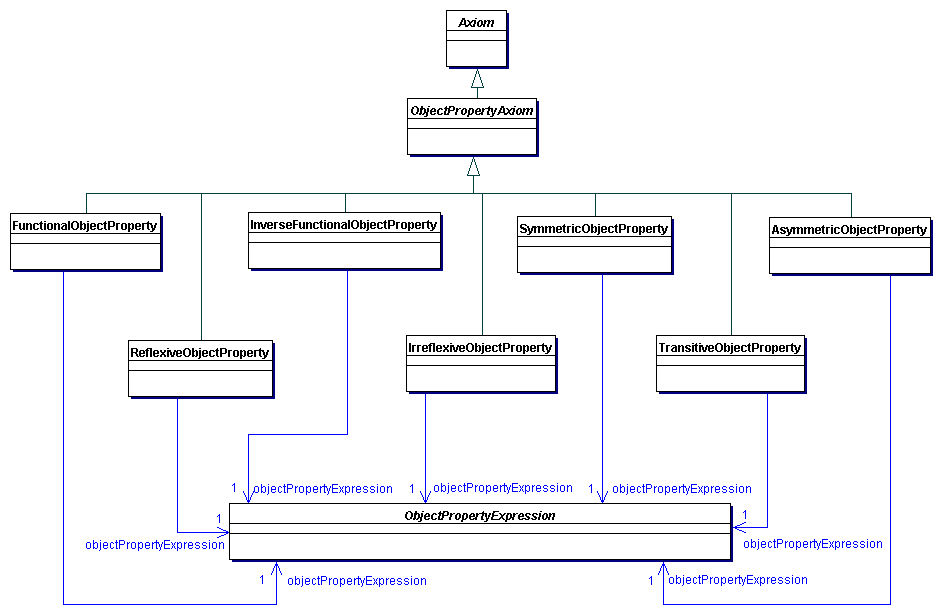
\includegraphics[width=150mm, height=100mm]{Figures/objectpropertyAxiom1.png}
		\caption{Các dạng phát biểu về thuộc tính đối tượng của OWL 2 (phần 2) \label{overflow}}
	\end{figure}
	Ngoài các dạng phát biểu được nêu, mô tả thuộc tính đối tượng còn có thêm các phát biểu trong hình sau, nhằm quy định tính chất của mô tả thuộc tính đối tượng hay giữa các cá thể được kết nối bằng các thuộc tính đối tượng này, chẳng hạn thuộc tính\textit{ SymmetricObjectProperty} quy định mô tả thuộc tính đối tượng có tính đối xứng - nếu $x$ là bạn $y$ thì $y$ cũng là bạn $x$. 
	
	\subparagraph{Functional Object Properties} phát biểu \textit{FunctionalObjectProperty( OPE )} quy định với từng cá thể $x$, chỉ tồn tại nhiều nhất một cá thể $y$ mà $x$ được kết nối với $y$ qua $OPE$. Ví dụ : Mỗi đối tượng chỉ có tối đa một người cha - \textit{FunctionalObjectProperty( a:hasFather )}. 
	
	\subparagraph{Inverse-Functional Object Properties} phát biểu \textit{InverseFunctionalObjectProperty( OPE )} quy định với từng cá thể $x$, chỉ tồn tại nhiều nhất một cá thể $y$ mà $y$ được kết nối qua \textit{OPE} tới $x$ . Ví dụ tương tự \textit{FunctionalObjectProperty(OPE)}.
	
	\subparagraph{Reflexive Object Properties} phát biểu \textit{ReflexiveObjectProperty( OPE )} nói rằng mô tả thuộc tính có tính phản xạ, nghĩa là với từng kết nối bởi \textit{OPE} tới chính nó. Ví dụ: \textit{ReflexiveObjectProperty(a:knows)}, ai cũng biết bản thân họ, với khai báo \textit{ClassAssertion(a:Person a:Peter)} thì có thể suy ra được phát biểu sau \textit{ObjectPropertyAssertion(a:knows a:Peter a:Peter)}.
	
	\subparagraph{Irreflexive Object Properties} ngược lại với phát biểu trên  \textit{IrreflexiveObjectProperty( OPE )}, không có cá thể nào tự kết nối với chính nó qua \textit{OPE}. Ví dụ: \textit{IrreflexiveObjectProperty(a:marriedTo)}, không ai cưới chính mình.
	
	\subparagraph{Symmetric Object Properties} phát biểu \textit{SymmetricObjectProperty( OPE )} nói rằng \textit{OPE} có tính đối xứng, nếu $x$ nối với $y$ qua \textit{OPE} thì $y$ cũng nối với $x$ bởi \textit{OPE}. Ví dụ: Với\textit{ SymmetricObjectProperty( a:friendOf )} và \textit{ObjectPropertyAssertion(a:friend a:Peter a:Bush)} chúng ta suy ra được \textit{ObjectPropertyAssertion(a:friend a:Bush a:Peter)}.
	
	\subparagraph{Asymmetric Object Properties} phát biểu \textit{AsymmetricObjectProperty( OPE )} nói rằng \textit{OPE} có tính bất đối xứng, nếu $x$ nối với $y$ qua \textit{OPE}, thì $y$ không thể kết nối với $x$ bởi \textit{OPE}. Ví dụ: Với \textit{AsymmetricObjectProperty( a:parentOf )}  và \textit{ObjectPropertyAssertion(a:parentOf a:Peter a:Bush)} thì nếu ta thêm thêm phát biểu \textit{ObjectPropertyAssertion(a:parentOf a:Bush a:Peter)} sẽ làm cho ontology mất tính nhất quán (inconsistent).
	
	\subparagraph{Transitive Object Properties} phát biểu \textit{TransitiveObjectProperty(OPE)} nói rằng \textit{OPE} có tính bắc cầu, nếu $x$ nối với $y$ bởi \textit{OPE} và $y$ nối với $z$ cũng bằng \textit{OPE} thì $x$ nối với $z$ qua \textit{OPE}. Ví dụ:
	\begin{verbatim}
	TransitiveObjectProperty( a:partOf ) 
	ObjectPropertyAssertion( a:partOf a:KhoaMMT a:UIT )
	ObjectPropertyAssertion( a:partOf a:UIT a:VNU )
	\end{verbatim}
	Giải thích nếu khoa mạng thuộc UIT, UIT thuộc đại học Quốc Gia (VNU), nhờ phát biểu đầu tiên chúng ta $partOf$ có tính chất bắc cầu nên suy ra được khoa mạng thuộc đại học Quốc Gia - \textit{ObjectPropertyAssertion( a:partOf a:KhoaMMT a:VNU)}
	
	% Data Property Axioms
	\paragraph{Phát biểu về thuộc tính dữ liệu (Data Property Axiom)}
	\begin{figure}[h]
		\centering
		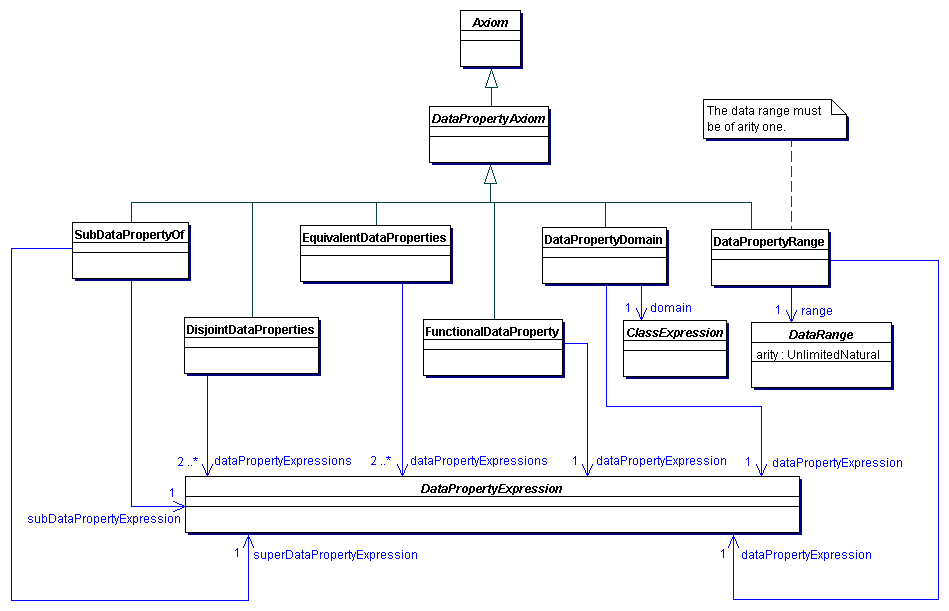
\includegraphics[width=150mm]{Figures/datapropertyAxiom.png}
		\caption{Các dạng phát biểu về thuộc tính dữ liệu của OWL 2 (phần 2) \label{overflow}}
	\end{figure}
	Cũng giống như mô tả thuộc tính đối tượng, mô tả thuộc tính dữ liệu cũng được cung cấp các phát biểu như \textit{SubDataPropertyOf}, \textit{EquivalentDataProperties}, \textit{DataPropertyDomain}, \textit{DataProperyRange}.
	
	\subparagraph{Phát biểu thuộc tính dữ liệu con (Data subproperties)} Phát biểu SubDataPropertyOf( $DPE_{1}$ $DPE_{2}$ ) nói rằng mô tả thuộc tính dữ liệu $DPE_{1}$ là thuộc tính con của mô tả dữ liệu $DPE_{2}$ - có nghĩa nếu một cá thể $x$ được kết nối bởi $DPE_{1}$ tới một trực nghĩa $y$, thì $x$ được kết nối bởi $DPE_{2}$. Ví dụ:
	\begin{verbatim}
	SubDataPropertyOf( a:hasLastName a:hasName) 
	// Họ của một người cũng là tên họ của người đó
	DataPropertyAssertion( a:hasLastName a:Peter "Smith" )
	// Họ của Peter là "Smith"
	\end{verbatim}
	\textbf{Giải thích:} Vì "có họ" \textbf{(hasLastName)} là thuộc tính con của "có tên" \textit{(hasName)} nên chúng ta ngầm hiểu phát biểu sau mà không cần khai báo tên của Peter là "Smith", tương đương \textit{DataPropertyAssertion(a:hasName a:Peter "Griffin")}
	
	\subparagraph{Phát biểu thuộc tính dữ liệu tương đương (Equivalent Data Properties)} Một phát biểu \textit{EquivalentDataProperties( $DPE_{1}$ ... $DPE_{n}$)} nói rằng mỗi mô tả thuộc tính $DPE_{i}$, $1<=i<=n$ đều đồng nghĩa với các tất cả các mô tả thuộc tính còn lại trong phát biểu này phát biểu \textit{EquivalentDataProperties( $DPE_{2}$ $DPE_{1}$ )} cũng tương đương \textit{EquivalentDataProperties( $DPE_{1}$ $DPE_{2}$ )}. Ví dụ:
	\begin{verbatim}
	EquivalentDataProperties( a:hasName a:HoTen ) 
	// a:hasName tương đượng với a:HoTen trong Tiếng Việt
	DataPropertyAssertion( a:hasName a:Peter "Peter Nguyen" )
	DataPropertyAssertion( a:HoTen a:Peter "Peter Nguyễn" )
	\end{verbatim}
	\textbf{Giải thích:} Do phát biểu đầu tiên, từ phát biểu thứ 2 ta ngầm hiểu \textit{DataPropertyAssertion( a:hasName a:Peter "Peter Nguyễn" )} tên tiếng Anh "Peter Nguyen" tương đương tên tiếng Viết "Peter Nguyễn" và ngược lại \textit{DataPropertyAssertion( a:HoTen $a:Peter$ "Peter Nguyen") }.
	
	\subparagraph{Domain của thuộc tính dữ liệu (Data Property Domain)} Phát biểu \textit{DataPropertyDomain( DPE CE )} nêu rõ domain của thuộc tính dữ liệu là mô tả lớp $CE$ -  nếu một cá thể $x$ được liên kết bởi \textit{DPE} tới vài trực nghĩa nào đó, thì $x$ phải là cá thể thuộc mô tả lớp \textit{CE}.
	\begin{verbatim}
	DataPropertyDomain( a:hasBankAccount a:Person ) 
	// Con người mới có tài khoản ngân hàng
	ObjectPropertyAssertion( a:hasBankAccount a:Peter "0002" ) 
	// Peter có tài khoản ngân hàng "0002"
	\end{verbatim}
	\textbf{Giải thích:} Không cần thiết phải khai báo Peter là người vì dựa theo chúng ta cũng kết luận được Peter là người từ 2 phát biểu trên, \textit{ClassAssertion(a:Person a:Peter)}.
	
	\subparagraph{Miền giá trị của thuộc tính dữ liệu (Data Property Range)} - phát biểu \textit{DataPropertyRange(DPE DR)} nói rằng miền giá trị hợp lệ của mô tả thuộc tính dữ liệu \textit{DPE} là miền dữ liệu \textit{DR} - nếu các cá thể được kết nối bởi \textit{DPE} tới 1 trực nghĩa $x$, thì $x$ trong miền dữ liệu \textit{DR}. Ví dụ:
	%Số lượng kết quả đầu ra bắt buộc bằng 1, tức không tồn tại $x \equiv y \equiv z$, với $y \not\equiv z$ và $y, z \in DR$.
	\begin{verbatim}
	DataPropertyRange( a:hasName xsd:string )
	DataPropertyAssertion( a:hasName a:Peter "Peter Nguyen" )
	\end{verbatim}
	Nếu khai báo thêm phát biểu sau sẽ làm cho ontology bị thiếu nhất quán (inconsistent):
	\begin{verbatim}
	DataPropertyAssertion( a:hasName a:Peter "42"^^xsd:integer)
	\end{verbatim}
	
	\subparagraph{Functional Data Properties} - phát biểu \textit{FunctionalDataProperty(DPE)} nói rằng với mỗi $x$, chỉ có nhiều nhất một trực nghĩa $y$ mà $x$ được gán cho bởi \textit{DPE}. Ví dụ:
	\begin{verbatim}
	FunctionalDataProperty( a:hasAge )
	// Mọi đối tượng chỉ có tối đa một số tuổi
	DataPropertyAssertion( a:hasAge a:Steve "17"^^xsd:integer )
	\end{verbatim}
	Các phát biểu trên sẽ bị thiếu nhất quán nếu chúng ta thêm vào phát biểu sau :
	\begin{verbatim}
	DataPropertyAssertion( a:hasAge a:Steve "15"^^xsd:integer)
	\end{verbatim}
	
	%% Assertions
	\paragraph{Các phát biểu về cá thể (Assertions)} 
	\begin{figure}[H]
		\centering
		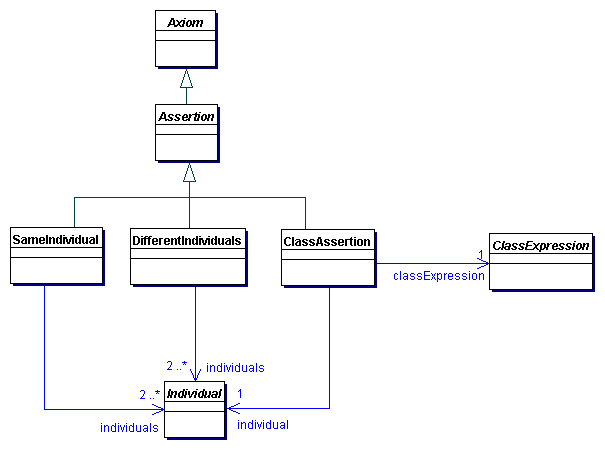
\includegraphics[width=120mm]{Figures/abox1.png}
		\caption{Các phát biểu gán lớp cho cá thể và cá thể giống nhau/khác nhau trong OWL 2 \label{overflow}}
	\end{figure}
	
	\begin{figure}[h!]
		\centering
		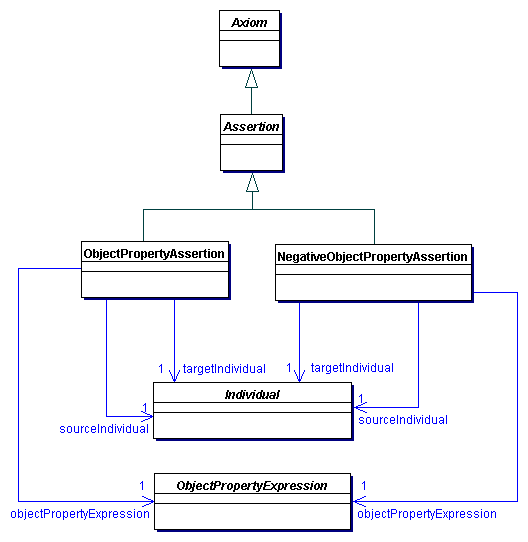
\includegraphics[width=120mm,height=110mm]{Figures/abox2.png}
		\caption{Các phát biểu về thuộc tính đối trượng của cá thể trong OWL 2 \label{overflow}}
	\end{figure}
	
	\begin{figure}[h!]
		\centering
		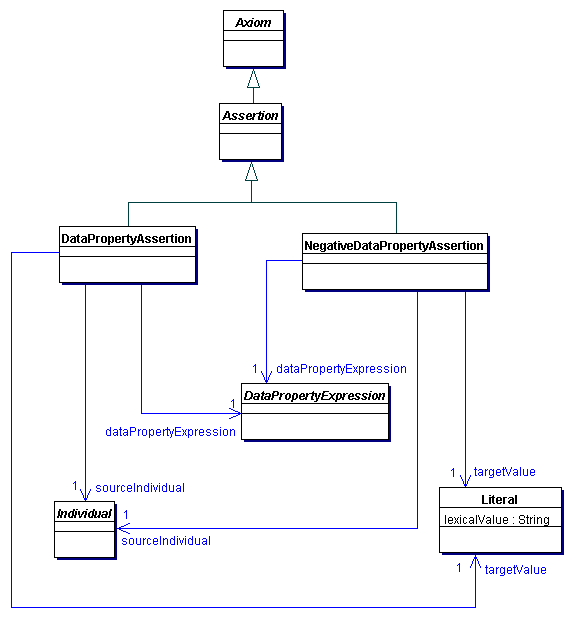
\includegraphics[width=120mm,height=110mm]{Figures/abox3.png}
		\caption{Các phát biểu về thuộc tính dữ liệu của cá thể trong OWL 2 \label{overflow}}
	\end{figure}
	Các phát biểu về cá thể thường được gọi là \textit{facts}. Để rõ hơn, các loại assertions khác nhau được thể hiện trong các hình sau.
	
	\begin{description}
		\item[SameIndividual] - khẳng định sự tương đồng của các cá thể trong phát biểu.
		
		\item[DifferentIndividuals] - khẳng định sự khác nhau của các cá thể trong phát biểu.
		
		\item[ClassAssertion] - khẳng định một cá thể thuộc một mô tả lớp/ lớp cụ thể trong phát biểu.
		
		\item[ObjectPropertyAssertion] - khẳng định mối quan hệ từ một cá thể tới một cá thể nào đó bởi một mô tả thuộc tính đối tượng.
		
		\item[NegativeObjectPropertyAssertion] - phủ định mối quan hệ từ một cá thể tới một cá thể khác bởi một mô tả thuộc tính đối tượng.
		
		\item[DataPropertyAssertion] - khẳng định mối quan hệ từ một cá thể tới một trực nghĩa bởi một mô tả thuộc tính dữ liệu.
		
		\item[NegativeDataPropertyAssertion] - phủ định mối quan hệ từ một cá thể tới một trực nghĩa bởi một mô tả thuộc tính dữ liệu.
	\end{description}
	
\paragraph{Kết luận} Chúng em vừa trình bày qua những thành phần chính của OWL2 cũng như cách sử dụng của chúng trong quá trình suy luận (reasoning) nhằm tìm ra thông tin ẩn bên trong những phát biểu được khai báo, với mục tiếu cuối cùng là trình bày tính năng phân loại tự động. Vì độ dài khóa luận hạn chế, nên có một số thành phần của OWL 2 chưa được nêu ra ở đây như \textbf{Datatype Definitions}, \textbf{Keys}, \textbf{Annotations}, \textbf{Datatype Maps}. Thầy cô và các bạn có thể tham khảo thêm ở \cite{owl2spec}. Phần tiếp theo chúng em xin được giới thiệu về Semantic Web Rule Language, một ngôn ngữ điều luật có nhiệm vụ chính là tăng cường tính năng suy luận cho ngôn ngữ OWL 2.
%% ----------------------------------------------------------------
% Kết thúc OWL
%% ----------------------------------------------------------------
% Bắt đầu SWRL 
%% ----------------------------------------------------------------
\section{Semantic Web Rule Language}
Nếu chỉ sử dụng các thành phần của OWL 2 được trình bày ở chương trước thì vẫn chưa đủ diễn tả hết tất cả các mối quan hệ trong ontology. Semantic Web Rule Language (SWRL) là một ngôn ngữ điều luật tuân theo các quy ước Description Logic mà OWL 2 tuân theo \cite{swrlfaq}. SWRL cho phép người sử dụng khai báo các điều luật dựa trên các khái niệm của OWL như lớp, thuộc tính đối tượng, thuộc tính dữ liệu nhằm cung cấp một khả năng suy luận mạnh mẽ hơn so với chỉ dùng OWL 2. SWRL có ưu điểm là giúp tối ưu khả năng lập luận, tuy nhiên nó cũng có nhược điểm là dễ làm cho các phát biểu bị thiếu nhất quán (inconsistent).

\subsection{Cấu trúc của một SWRL Rule \cite{swrlfaq}}
Một luật SWRL chứa một phần điều kiện, hay còn gọi là rule body, và một phần kết quả, hay còn gọi là rule head. Cả phần body và head đều là giao của các positive atoms.
\begin{center}
	$atom$ \verb|^| $atom$ ... -> $atom$ \verb|^| $atom$ 
\end{center}
Có thể hiểu một SWRL Rule theo cách như sau : Khi tất cả các điều kiện nhỏ nhất (atom) trong phần điều kiện (body) đúng thì chắc chắn rằng những ý được nêu ra trong phần kết quả (head) cũng đúng. Một rule \textit{atom} có dạng:
\begin{center}
	$p($ $arg_{1}$, $arg_{2}$, ... $arg_{n}$ $)$
\end{center}
Trong đó $p$ là kí hiệu cho nội dung điều kiện (Predicate) và $arg_{i}$, $1<=i<=n$, là những khái niệm hay tham số của một \textit{Rule Atom}. Trong SWRL, nội dung điều kiện có thể là các lớp, các thuộc tính hoặc kiểu dữ liệu trong OWL 2. Tham số truyền vào có thể là cá thể, giá trị dữ liệu, hoặc biến để gán cho các khái niệm vừa nêu. Tên biến chỉ có hiệu lực trong cùng một rule, vì vậy có thể sử dụng lại tên biến cho 2 rule khác nhau.
\subsection{Các loại Rule Atom}
Sau đây, chúng em xin trình bày các loại \textit{Atom} trong SWRL Rule, đồng thời kèm theo những ví dụ cơ bản thể hiện tính năng quyết định dựa trên các điều kiện của SWRL.
\subsubsection{Class Atom}
Một \textbf{Class Atom} gồm một tên lớp hay mô tả lớp trong OWL2 Ontology và một tham số duy nhất đại diện cho cá thể của lớp đó. Ví dụ:
\begin{verbatim}
Person(?p)
Vehicle(?v)
Man(Peter)
\end{verbatim}
Tham số có thể là biến đại diện cho cá thể \verb|?p|, \verb|?v| hoặc tên của cá thể \verb|Peter|.
Một rule đơn giản để khẳng định rằng "ai là nam đều là người":
\begin{verbatim}
Man(?x) -> Person(?x)
\end{verbatim}
\subsubsection{Individual Property Atom}
Một \textbf{Individual Property Atom} gồm một thuộc tính đối tượng (object property) và 2 tham số đại diện cho 2 cá thể trong OWL2 ontology, tham số có thể là biến hoặc tên của cá thể. Ví dụ:
\begin{verbatim}
hasBrother(?x, ?y)   // có anh em
hasSibling(Steve, ?y) // có anh/chị em 
\end{verbatim}
Trong ví dụ, \textit{hasBrother} và \textit{hasSibling} là các thuộc tính đối tượng, \verb|?x| và \verb|?y| là biến đại diện cho các cá thể, và \verb|Steve| là tên của một cá thể (named individual). Xem ví dụ sau:
\begin{verbatim}
Person(?p) ^ hasSibling(?p,?s) ^ Man(?s) -> hasBrother(?p,?s)
\end{verbatim}
\textbf{Giải thích:} Nếu một người \verb|?p| nào đó có một anh chị em \verb|?s| nào đó, và người \verb|?s| này là nam thì người \verb|?p| có anh/em trai là người \verb|?s|. Rule này cũng có thể được biểu diễn trong bằng các phát biểu về lớp, domain và range OWL2 như sau:
\begin{verbatim}
SubClassOf(a:Man a:Person)
SubClassOf(a:Woman a:Person)
DisjointClasses(a:Woman a:Man)
SubObjectProperty(a:hasBrother a:hasSibling)
ObjectPropertyRange(a:hasBrother a:Man)
ObjectPropertyRange(a:hasSibling a:Person)
ObjectPropertyDomain(a:hasSibling a:Person)
ObjectPropertyDomain(a:hasBrother a:Person)
\end{verbatim}
Trong trường hợp chúng ta có các khẳng định sau về 2 cá thể \verb|Peter| và \verb|Nguyen|
\begin{verbatim}
ClassAssertion(a:Person a:Peter)
ClassAssertion(a:Man a:Nguyen)
ObjectPropertyAssertion(a:hasSibling a:Peter a:Nguyen)
\end{verbatim}
Dựa vào rule đã khai báo ở trên \textit{hoặc} các phát biểu về lớp, domain, range như trên, thì các khẳng định vừa nêu sẽ suy ra cùng một kết quả đó là "Peter có anh/em trai là Nguyen" tương đương với phát biểu \textit{ObjectProperyAssertion(a:hasBrother a:Peter a:Nguyen)}.
\\
\textbf{Nhận xét:} Qua các ví dụ này, có thể thấy rõ ràng SWRL có lợi thế hơn trong việc suy ra các ẩn ý so với việc chỉ sử dụng các phát biểu của OWL2, tuy nhiên có một nhược điểm đó là tính nhất quán (consistency) của ontology dễ bị vi phạm hơn do rule có thể xung đột với các phát biểu của OWL2. Lấy lại các phát biểu và rule trong ví dụ trên:
\begin{verbatim}
Person(?p) ^ hasSibling(?p,?s) ^ Woman(?s) -> hasBrother(?p,?s)
Person(?p) ^ hasSibling(?p,?s) ^ Man(?s) -> hasBrother(?p,?s)
ObjectPropertyRange(a:hasBrother a:Man) // Có anh/em trai
\end{verbatim}
\textbf{Giải thích:} 2 Rule mâu thuẫn với nhau do phát biểu "có anh/em trai". Bản thân SWRL sẽ không kiểm tra các mâu thuẫn này cho đến khi chúng xảy ra và làm cho ontology bị thiếu nhất quán. Vì vậy, người phát triển ontology cần cẩn thận trong việc kết hợp cả SWRL và OWL2.

\subsubsection{Data Valued Property Atom}
Một Data Valued Property Atom gồm một thuộc tính dữ liệu trong OWL2 và 2 tham số. Tham số đầu tiên được gán cho một các thể trong OWL 2, có thể là biến số hay tên của cá thể. Tham số thứ hai gán cho một giá trị dữ liệu, có thể là biến số hay giá trị. Ví dụ:
\begin{verbatim}
hasAge(?x, ?age)
hasName(?x, "Nguyen")
hasNumberOfChilds(Peter, ?x)
\end{verbatim}
Một rule đơn giản với ý nghĩa "những ai có xe, có bằng lái thì là tài xế":
\begin{verbatim}
Person(?p) ^ hasCar(?p, true) ^ hasLicense(?p, true) -> Driver(?p)
\end{verbatim}
Chúng ta cũng có thể dùng tên của cá thể cụ thể:
\begin{verbatim}
Person(Steve) ^ hasCar(Steve, true) ^ hasLicense(Steve, true) -> Driver(Steve)
\end{verbatim}
Rule này chỉ có tác dụng duy nhất lên cá thể \verb|Steve|.

\subsubsection{Different Individuals Atom}
Một \textit{Atom} dạng này gồm cú pháp \textit{differentFrom} với 2 tham số đại diện cho 2 cá thể. Ví dụ:
\begin{verbatim}
differentFrom(?x, ?y)
differentFrom(Steve, Peter)
\end{verbatim}

\subsubsection{Same Individuals Atom}
Một \textit{Atom} dạng này gồm cú pháp \textit{sameAs} với 2 tham số đại diện cho 2 cá thể. Ví dụ:
\begin{verbatim}
sameAs(?x, ?y)
sameAs(Steve, Peter)
\end{verbatim}

\subsubsection{Data Range Atom}
Một Data Range Atom gồm một dạng dữ liệu hoặc một tập hợp các trực nghĩa (literals) và duy nhất một tham số đại diện cho giá trị dữ liệu. Ví dụ:
\begin{verbatim}
xsd:int(?x)
xsd:string(?x)
[3,2,1](?x)
xsd:int[>=5,<=9](?x)
\end{verbatim}

\subsubsection{Những Built-in Atom}
Một trong những tính năng mạnh nhất của SWRL chính là khả năng hỗ trợ người phát triển tự xây dựng các built-in nhằm mở rộng khả năng ra các điều kiện cho SWRL Rule. Trong phạm vi khóa luận, chúng em sẽ không đề cập đến cách xây dựng các SWRL Built-in \cite{swrlbuiltin}, mà chỉ sử dụng những core built-in \cite{swrlcorebuiltin} có sẵn để xây dựng nên tính năng phân loại. Dưới đây là một ví dụ về core built-in. Để có nhiều thông tin hơn mời thầy cô và các bạn đọc thêm ở \cite{swrlcorebuiltin}.
\paragraph{Built-In dùng cho các phép so sánh}
\begin{table}[!h]
	\centering
	\begin{tabular}{|l|l|l|}
		\hline
		Cú pháp & Ví dụ & Ý nghĩa \\ 
		\hline
		swrlb:equal & swrlb:equal(?x,9) & $x = 9$  ? \\		
		\hline
		swrlb:notEqual & swrlb:notEqual(?x,9) & $x \neq 9$  ? \\		
		\hline
		swrlb:lessThan & swrlb:lessThan(?x, 9) & $x < 9$ ? \\
		\hline
		swrlb:lessThanOrEqual & swrlb:lessThanOrEqual(?x, 9) & $x <= 9$ ? \\
		\hline
		swrlb:greaterThan & swrlb:greaterThan(?x, 9) & $x > 9$ ? \\
		\hline
		swrlb:greaterThanOrEqual & swrlb:greaterThanOrEqual(?x, 9) & $x >= 9$ ? \\
		\hline
	\end{tabular}
	\caption{Built-In dùng để so sánh\label{overflow}}
\end{table}
Ví dụ:
\begin{verbatim}
Person(?p) ^ hasAge(?p, ?age) ^ swrlb:greaterThan(?age, 17) -> Adult(?p)
Vehicle(?v) ^ canCarryNumberOfPassenger(?v, ?x) ^ 
swrlb:greaterThan(?x, 30) -> Bus(?v)
\end{verbatim}
%% ----------------------------------------------------------------
% Kết thúc SWRL 
%% ----------------------------------------------------------------
% Bắt đầu Ontology Consistency
%% ----------------------------------------------------------------
\section{Tính nhất quán của một ontology}
Khái niệm tính nhất quán (consistency) đã được nhắc đến nhiều lần trong những phần trước. Vậy tính nhất quán là gì và nó có ảnh hưởng như thế nào đến một mô hình ontology. 
\\
\textbf{Trả lời:} Tính nhất quán chỉ sự thống nhất về ý nghĩa của những phát biểu trong ontology hay ý nghĩa của những phát biểu này không mâu thuẫn với nhau. Tính nhất quán cực kì quan trọng đối với bất kì một ontology nào, nếu ngữ nghĩa của của những phát biểu trong ontology đã tồn tại sự mâu thuẫn thì những thông tin được suy luận ra từ những phát biểu này cũng trở nên vô lý. Chính vì thế, quá trình suy luận (reasoning) sẽ không thực hiện được nếu ontology không có tính nhất quán. Trong phần này, chúng em xin được nêu ra các nguyên nhân phổ biến làm cho các phát biểu khai báo mâu thuẫn với nhau, qua đó sẽ giúp chúng ta tránh phải những lỗi này khai phát triển ontology.

\subsection{Các định nghĩa cần lưu ý \cite{satisfy}}
% Định nghĩa Unsatisfiable Class
\paragraph{Lớp không hợp lý - Unsatisfiable Class} Dùng để chỉ một lớp mà các phát biểu mô tả, khai báo về nó có ý nghĩa mâu thuẫn với nhau.
\subparagraph{Ví dụ}
	\begin{verbatim}
	Cow	SubClassOf: 	Vegetarian
	Vegetarian	SubClassOf: Animal and eats only Plant
	DisjointClasses:	Plant, Animal
	MadCow 	SubClassOf: Cow and eats some Sheep
	Sheep 	SubClassOf: Animal
	Individual: Dora type: MadCow
	\end{verbatim}
\subparagraph{Giải thích} Trong ví dụ trên thì \textit{MadCow} là một lớp không hợp lý do ý nghĩa các phát biểu về nó mâu thuẫn với nhau. Cow là lớp con của \textit{Vegeterian}, mà \textit{Vegeterian} chỉ ăn Plant (từ \textit{only} đồng nghĩa với \textit{AllValuesFrom} được giải thích trong phần OWL 2). Trong khi đó khai báo của lớp \textit{MadCow} là lớp con của \textit{Cow} và mô tả ăn (eats some - từ \textbf{some} tương đương \textit{SomeValuesFrom}) \textit{Sheep} (Sheep là một lớp con của Animal). Từ đây, suy luận từ các phát biểu trên sẽ có khả năng sinh ra mâu thuẫn: Sheep cũng có khả năng là một phần của Plant (do phát biểu \textit{eats only plant}). Một điểm lưu ý với phát biểu DisjointClasses thì Plant và Animal luôn được khẳng định là khác nhau, nói cách khác không tồn tại một cá thể nào vừa thuộc lớp Plant và vừa thuộc lớp Animal, điều này mâu thuẫn với phát biểu ở câu trước.  

% Định nghĩa về Incoherent Ontology 
\paragraph{Ontology có ý nghĩa không mạch lạc - Incoherent Ontology} Dùng để chỉ một \textit{ontology/model} có ý nghĩa không mạch lạc rõ ràng do nó có chứa ít nhất một lớp không hợp lý \textit{Unsatisfiable Class} và với điều kiện là trong những \textit{Unsatisfiable Class} này không được chứa bất kì một cá thể nào. Giả sử ta có ontology A chứa các phát biểu trong ví dụ trên ngoại trừ phát biểu cuối cùng \texttt{Individual: Dora type: MadCow} thì ta có thể nói ontology A không mạch lạc rõ ràng do nó chứa unsatisfiable class là MadCow. Chúng ta vẫn có thể sử dụng được ontology A vì nó vẫn còn tính nhất quán (\textit{Consistency}) miễn là không có phần tử nào thuộc lớp MadCow.
% Định nghĩa về Inconsistent Ontology
\paragraph{Ontology không có tính nhất quán - Inconsistent Ontology} Một ontology không nhất quán khi đạt đủ 2 điều kiện: có ít nhất một lớp không hợp lý và có ít nhất một cá thể là thành viên của một trong những lớp không hợp lý này. Như đã thể hiện trong ví dụ đầu tiên thì cá thể \textit{Dora} thuộc lớp \textit{MadCow} (Một lớp không hợp lý thì không nên tồn tại bất kì cá thể nào nếu như chúng ta muốn đảm bảo tính nhất quán cho ontology). Lưu ý: một ontology không nhất quán thì không được dùng để suy luận vì những suy luận từ đây có khả năng đều bất hợp lý.

\subsection{Các nguyên nhân phổ biến dẫn đến tính thiếu nhất quán}
Các nguyên nhân dẫn đến tính thiếu nhất quán trong ontology gây bởi các lỗi được phân loại thành lỗi gây ra bởi phát biểu ở mức độ lớp (Class level - TBox), các lỗi gây ra bởi phát biểu ở mức độ cá thể (Instance/Individual level - ABox)\cite{inconsitentReason} và lỗi gây ra bởi sự kết hợp của cả 2 nguyên nhân vừa nêu trên.
{
	\let\thefootnote\relax\footnotetext{
		* TBox\textit{
			Chỉ những phát biểu liên quan đến lớp
		}}		
		\let\thefootnote\relax\footnotetext{
		  ABox: \textit{Chỉ những phát biểu liên quan đến cá thể}
		}
}
% Instantiating an unsatisfiable class (TBox + ABox)
\paragraph{Khởi tạo cá thể cho một lớp không hợp lý - (TBox + ABox)\textsuperscript{*}} Khởi tạo cá thể cho một Unsatisfiable Class được xem là nguyên nhân phổ biến nhất gây ra tính thiếu nhất quán trong ontology. Ví dụ:
\begin{verbatim}
	Individual: Dora type: MadCow
\end{verbatim}
Như đã giải thích ở phần trên, một lớp không hợp lý thì không nên tồn tại bất kì cá thể nào nếu như chúng ta muốn đảm bảo tính nhất quán cho ontology.

% Instantiating disjoint classes (TBox + ABox)
\paragraph{Khởi tạo cá thể thuộc 2 class được disjoint với nhau (TBox + ABox)} Đây là một trường hợp dễ bắt gặp vì nó sai ngay trong phát biểu về logic.
\begin{verbatim}
DisjointClasses: Animal, Plant
Individual: Cat Types: Animal, Plant
\end{verbatim}
Bản thân phát biểu Disjont đã khẳng định 2 lớp \textit{Animal}, \textit{Plant} sẽ không bao giờ có cá thể chung nên phát biểu thứ 2 đã mâu thuẫn với nó.

% Conflicting assertions (ABox)	
\paragraph{Các phát biểu về cá thể (ABox) mâu thuẫn với nhau} Trường hợp này thì tương tự như nguyên nhân ở trên nhưng khác ở chỗ là lần này sự mâu thuẫn nằm trong các biểu ở cấp độ cá thể (ABox). Ví dụ:	
\begin{verbatim}
Individual: Cat Types: Animal, not Animal
\end{verbatim}

% Conflicting axioms with nominals (all TBox)
\paragraph{Phát biểu "oneOf" về lớp (TBox)} Phát biểu bao gồm hoặc một trong (phát biểu liệt kê cá thể ObjectOneOf) cho phép khai báo các cá thể (ABox) thuộc một lớp. Sự kết hợp này đôi khi dẫn đến sự thiếu nhất quán. Lấy ví dụ sau:
\begin{verbatim}
Class: MyFavouriteCat EquivalentTo: {Tom}
Class: AllMyCats EquivalentTo: {Tom, Jerry}
DisjointClasses: MyFavouriteCat, AllMyCats
\end{verbatim}
Chúng ta có diễn giải sau đây \textit{MyFavouriteCat} tương đương \textit{{Tom}}, \textit{AllMyCats} tương đương \textit{{Tom, Jerry}}, \textit{MyFavouriteCat} và \textit{AllMyCats} không được có chung cá thể nào. Nhưng rõ ràng thì \textit{Tom} là cá thể chung của 2 lớp vì vậy các phát biểu này mâu thuẫn.


% No instantiation possible (all TBox)
%\paragraph{Không có khả năng khởi tạo bất kì cá thể nào (all TBox)}
%Ví dụ:
%\begin{verbatim}
%Vegetarian or not Vegetarian SubClassOf: Cow and not Cow
%\end{verbatim}
%Đây chỉ là một ví dụ đơn giản để minh họa cho trường hợp này. Thực tế sẽ ít người dùng nào tạo ra một phát biểu ngớ ngẩn như vậy nhưng nó vẫn có khả năng xảy ra khi phát biểu trên là kết quả từ suy luận (reasoning) của những phát biểu lớn và phức tạp hơn đặc biệt khi trong chúng.
%\\
%\textbf{Giải thích} \texttt{Vegetarian} hoặc không phải \texttt{Vegetarian} - bất kỳ phát biểu nào dạng này, "cá thể thuộc hoặc không thuộc một lớp" chỉ tất cả cá thể tồn tại trong ontology. Dòng thứ hai yêu cầu cá thể vừa là Cow vừa không phải là Cow, phát biểu này rơi vào một trong các nguyên nhân vừa nêu ở trên. Tổng hợp lại chúng yêu cầu tất cả cá thể vừa là Cow vừa không phải Cow, điều này gây ra mâu thuẫn trên toàn ontology do phát biểu đầu tiên chỉ tới tất cả các cá thể.

\paragraph{Kết luận}
Trên đây chúng em đã liệt kê những nguyên nhân phổ biến dẫn đến thiếu nhất quán qua những ví dụ đã được đơn giản hoá để dễ dàng nắm bắt được đâu là căn nguyên gây ra sự mâu thuẫn về logic. Trên thực tế với những ontology có số lượng phát biểu lớn và phức tạp rất khó để người dùng có thể nhận diện được đâu là các phát biểu mâu thuẫn trước khi nó gây ra sự thiếu nhất quán. Chúng ta thường sử dụng các công cụ phổ biến để tìm các lớp không hợp lý là debugger (được hỗ trợ trong các thư viện OWL-API, Pellet, Jena) và trên hết là sự cẩn thận của người phát triển ontology để hạn chế việc gây ra tính thiếu nhất quán trong ontology. Trong quá trình tìm hiểu chúng em cũng có đọc được các bài báo hay, trong đó đề ra các giải pháp để sửa chữa các lớp bất hợp lý và tìm giải thích cho chúng, tuy nhiên do trong phạm vi khóa luận chúng em cũng không thể giới thiệu được, thầy cô và các bạn có thể tham khảo thêm ở \cite{repair}, \cite{axiomPinpoint} và \cite{matt_horridge}. Trên đây là toàn bộ những kiến thức đã tìm hiểu được mà chúng em tin rằng nếu không nắm được chúng thì việc phát triển ontology và thao tác với thư viện lập trình liên quan đến ngôn ngữ OWL sẽ gặp rất nhiều khó khăn.

%% ----------------------------------------------------------------
% Kết thúc  Ontology Consistency 
%% ----------------------------------------------------------------
% Bắt đầu Explanation Generation
%% ----------------------------------------------------------------
%\section{Tạo ra các giải thích cho các suy luận tìm được}
%\paragraph{Giới thiệu} Bên cạnh việc suy luận ra các thông tin mới, thì việc tìm hiểu xim đâu là những lý do hay điều kiện để suy ra chúng cũng rất quan trọng trong việc tìm hiểu ý nghĩa của các phát biểu trong ontology. Nội dung phần này, chúng em xin trình bày những giải pháp tạo ra các giải thích cho một suy luận.
%\subsection{Các giải pháp tạo ra giải thích}
%\subsubsection{Tính năng Axiom Pinpointing}
%\paragraph{Axiom Pinpointing Service} là dịch vụ có khả năng thực hiện tác vụ giải thích vừa được đề cập, với một KB và bất kì kết quả suy luận nào từ KB, dịch vụ này sẽ trả về tập các chứng minh/giải thích cho suy luận đó bằng những phát biểu đã được khai báo trong KB.
%\\
%\hspace*{0.05\textwidth} Có thể giải thích ngắn gọn như sau \cite[p.~2]{axiomPinpoint}, cho một phát biểu kết quả họ SHOIN $\alpha$ được suy ra từ một knowledge base $K$, một kiểm chứng (justification) cho $\alpha$  trong $K$ là một phần tối tiểu $K^{'}\subseteq$ $K$ chịu trách nhiệm cho $\alpha$ xảy ra. Kiểm chứng $K^{'}$ là tối tiểu với điều kiện $\alpha$ là một kết quả logic được suy ra từ $K^{'}$, hay nói cách khác $K^{'}$ tối tiểu khi và chỉ khi bất kì tập con nào của $K^{'}$ đều không suy ra được $\alpha$. Nói chung có thể tồn tại nhiều giải thích/chứng minh cho $\alpha$ trong $K$. Sau đây là một ví dụ cho ý tưởng vừa nêu. Cho KB $K$ với các phát biểu như sau:
%\begin{enumerate}
%	\item	$A$ $\subseteq$ $B$ $\cap$ $C$ 
%	\item	$B$ $\subseteq$ $\neg$ $E$
%	\item	$A$ $\subseteq$ $D$ $\cap$ $\exists$ $R.E$ 
%	\item	$D$ $\subseteq$ $C$ $\cap$ $\forall$ $R.B$
%\end{enumerate}
%
%Trong KB trên, $A, B, C, D, E$ là atomic concepts và $R$ là atomic role.  Chúng ta sẽ dùng số thứ tự của từng câu phát biểu trên thay vì lặp lại nguyên văn.
%
%\hspace*{0.05\textwidth} Từ các phát biểu trên ta có $K$ $\models$ ($A$ $\subseteq$ $C$). Tuy nhiên, điều kiện cần và đủ để suy ra được một kết quả tương tự từ 2 phần nhỏ hơn của KB $K$ là $K_{1}$ = {1} và $K_{2}$ ={3,4}. Chúng ta nói $K_{1}$ và $K_{2}$ là các kiểm chứng cho kết luận nói $C$ là tập con của $A$ - $A$ $\subseteq$ $C$.
%
%\hspace*{0.05\textwidth} KB trong ví dụ vừa nêu được xem là khá nhỏ, qua đó dễ dàng nhận ra lợi ích đáng kể khi số lượng phát biểu trong KB tăng lên vài trăm hay vài ngàn phát biểu. Bằng cách nhận dạng chính xác các tập tối tiểu chứa các phát biểu khẳng định (asserted) là những giả thiết cho kết quả được suy ra, dịch vụ này có thể được dùng để cô lập, đánh dấu và giải thích nguyên nhân hoặc cơ sở của các kết quả suy luận. Điều này cực kì quan trọng trong khía cạnh debugging, lấy ví dụ trường hợp cần giải thích là một Unsatisfiable Class/Concept, dịch vụ này sẽ khám phá tất cả và chỉ những phát biểu là nguyên nhân gây lỗi. Trong trường hợp vừa nêu, tìm kiếm tất cả các kiểm chứng là rất cần thiết vì để sửa lại Unsatisfiable Class cần loại bỏ ít nhất một phát biểu trong tập các phát biểu tối tiểu nguyên nhân gây lỗi MUPS - sẽ được đề cập trong mục bên dưới.
%
%\hspace*{0.05\textwidth} Tuy nhiên, dịch vụ Axiom Pinpointing chúng ta đề cập có một giới hạn là nó chỉ làm việc ở mức độ giữa các phát biểu với nhau, chúng vẫn chưa phân biệt được phần cụ thể nào của phát biểu mới là nguyên nhân cần và đủ để giải thích cho kết quả suy luận. Lấy lại ví dụ vừa nếu trên KB $K$, lớp $B$ trong giao của $B$ $\cap$ $C$ trong phát biểu 1, không phải là giải thiết cần để suy ra $A$ $\subseteq$ $C$. Tương tự, $\exists$ $R.E$ và $\forall$ $R.B$ trong phát biểu 3 và 4 không phải điều kiện cần để suy ra được $A$ $\subseteq$ $C$. 
%
%\hspace{0.05\textwidth} Do vậy, việc quan tâm xem phần nào của phát biểu mới chính là giả thiết/nguyên nhân của kết quả suy luận rất quan trọng trong nhiều trường hợp, đặc biệt khi sửa chữa một phát biểu gây lỗi thì việc sửa lại một phần của phát biểu sẽ hạn chế sự mất mát về ý nghĩa của ontology hơn là xóa nó đi.
%
%\hspace*{0.05\textwidth} Để đáp ứng yêu cầu này, họ đã định nghĩa một \textit{hàm chia nhỏ KB}. Ý tưởng là viết lại một phát biểu bất kì trong KB thành những dạng tập gồm các phát biểu nhỏ và đơn giản hơn với ý nghĩa  tương đương. Sau đó, sử dụng \textit{Axiom Pinpointing Service} lên những tập những phát biểu trong KB $K_{s}$ đã được viết lại từ $K$ để tìm kiếm nguyên nhân hay giải thích cho kết quả suy luận. Lấy phát biểu 1 trong ví dụ trên:
%\begin{center}
%	$A$ $\subseteq$ $B$ $\cap$ $C$ (1) được viết lại thành $A$ $\subseteq$ $B$, $A$ $\subseteq$ $C$ (1\textsuperscript{*})
%\end{center}
%Dễ dàng thấy phần $A$ $\subseteq$ $C$ trong 1\textsuperscript{*} chính là điều phải chứng minh cho $K$ $\models$ ($A$ $\subseteq$ $C$), những phần còn lại không cần thiết. Tương tự, ta viết lại (3) và (4) như sau:
%\begin{center}
%	$A$ $\subseteq$ $D$ $\cap$ $\exists$ $R.E$  $\Leftrightarrow$ $A$ $\subseteq$ $D$, $A$ $\subseteq$ $\exists$ $R.E$
%	\\
%	$D$ $\subseteq$ $C$ $\cap$ $\forall$ $R.B$ $\Leftrightarrow$ $D$ $\subseteq$ $C$, $D$ $\subseteq$ $\exists$ $R.B$
%\end{center}
%Bây giờ, điều kiện cần và đủ để chứng minh $K$ $\models$ ($A$ $\subseteq$ $C$) là $A$ $\subseteq$ $D$ và $D$ $\subseteq$ $C$. Tuy nhiên, trong một vài trường hợp "hàm chia nhỏ KB" này đòi hỏi phải giới thiệu ra một tên lớp mới, viết giới thiệu tên lớp mới này chỉ phục vụ cho mục đích viết lại phát biểu. Ví dụ:	
%\begin{center}
%	$A$ $\subseteq$ $\exists$ $R.$ ($C\cap$ $D$) không tương đương với $A$ $\subseteq$ $\exists$ $R.C$, $A\subseteq$ $\exists$ $R.D$
%\end{center}
%Để chia nhỏ phát biểu trên chúng ta sẽ giới thiệu một tên lớp mới, gọi là $E$.	Như vậy ta có:
%\begin{center}
%	$A$ $\subseteq$ $\exists$ $R.$ ($C$ $\cap$ $D$) $\Leftrightarrow$ $A\subseteq$ $\exists$ $R.E$, $E\subseteq$ $C$, $E\subseteq$ $D$, $C\cap$ $D\subseteq$ $E$
%\end{center}
%Để thực hiện được cái gọi là \textit{"hàm chia nhỏ KB"} các bài báo \cite{repair} và \cite{axiomPinpoint} đã đề xuất các giải thuật với tiêu chí xác định các phát biểu chứng minh một cách đầy đủ và chính xác. Các giải thuật này có thể được chia thành 2 nhóm:
%\begin{enumerate}
%	\item \textit{Reasoner Dependent(or Glass-box) Algorithm} Đây là nhóm các giải thuật xây dựng trên quy trình đưa ra quyết định Tableau dành cho Description Logic. Tuy nhiên, để áp dụng các giải thuật loại này trong thực tế đòi hỏi phải có những chỉnh sửa đáng kể bên trong quy trình suy luận những DL reasoner hiện nay.
%	\item \textit{Reasoner Independent(or Black-box) Algorithm} Nhóm này chỉ sử dụng các DL reasoner cho những tác vụ kiểm tra lại kết quả suy luận khi đã viết lại KB $K$ thành $K^{'}$, chúng không đòi hỏi phải chỉnh sửa lại các cách hoạt động của reasoner. Reasoner lúc này có chức năng như một "chiếc hộp đen" chấp nhận các input là lớp/các phát biểu đã được viết lại hoặc một KB $K^{'}$ viết lại từ KB $K$, sau đó trả về output là một câu trả lời xác nhận hay phủ định rằng các lớp và các phát biểu này có là tập tối tiểu để chứng minh cho kết quả suy luận hay không. Ví dụ trong trường hợp:
%	\begin{center}
%		$A$ $\subseteq$ $B$ $\cap$ $C$ $\Leftrightarrow$ $A$ $\subseteq$ $B$, $A$ $\subseteq$ $C$
%	\end{center}
%	Các inputs của reasoner sẽ lần lượt sau mỗi vòng là 
%	\begin{enumerate}
%		\item $A$ $\subseteq$ $B$, $A$ $\subseteq$ $C$
%		\item $A$ $\subseteq$ $B$
%		\item $A$ $\subseteq$ $C$
%	\end{enumerate}
%	Giải thuật sẽ lần lượt loại bỏ từng phát biểu một (sau mỗi vòng) để xem những phát biểu còn lại có đủ chứng minh  $K$ $\models$ ($A$ $\subseteq$ $C$). Đến khi nào giải thuật không tồn tại tập phát biểu nào đủ để chứng minh $K$ $\models$ ($A$ $\subseteq$ $C$) thì sẽ dừng vòng lặp.
%\end{enumerate}
%\textbf{Kết luận:} Trên đây chỉ là những bước hoạt động cơ bản nhất của Axiom Pinpointing Service và Blackbox Algorithm, chi tiết khác xin đọc thêm \cite{axiomPinpoint}. Các giải thuật và dịch vụ này cũng đã được áp dụng trong package com.clarkparsia.owlapi.explanation của \cite{owowlapi} sẽ được giới thiệu ở chương sau.
%\subsubsection{Ứng dụng Hitting Set Tree để xác định tất cả giải thích cho suy luận\cite{matt_horridge}}
%Một giải pháp thứ hai là sử dụng giải thuật Hitting Set Tree \cite{hst} để tìm tất cả các giải thích với thời gian được tối ưu so với Axiom Pinpointing.	\hspace*{.05\textwidth} Với ontology $\beta$ $\models$ $\eta$, một cây hitting set (HST) cho $\eta$ trong $\beta$ là một cây hữu hạn, bao gồm node được dán nhãn bằng các kiểm chứng (justifications) hay các phát biểu chứng minh $\beta$ $\models$ $\eta$ và cạnh được đánh dấu với phát biểu trong $\beta$. Từng non-leaf(không phải lá) node $v$ nối với một node kế cận $v^{'}$ qua một cạnh được dán nhãn với một phát biểu $\alpha$ với $\alpha$ nẳm trong nhãn của $v$, nhưng không nằm trong nhãn của $v^{'}$. Nhãn của $v^{'}$ có thể là một tập hợp rỗng, trong trường hợp đó $v^{'}$ phải là node lá (leaf node). Ngoài ra, với bất kì node $v^{''}$, tập chứa các phát biểu dán nhãn cho đường đi từ $v^{''}$ tới gốc cây (tree root) \textit{không} giao với kiếm chứng(hay các phát biểu chứng minh) dán nhãn $v^{''}$.
%		
%\hspace*{.05\textwidth} Quá trình xây dựng HST có thể được thực hiện bằng các giải thuật \textit{breadth first} hay \textit{depth first}. Dù được sử dụng theo cách nào, các nguyên lý và các luật để tạo và dán nhãn cạnh, node trên cây đều như nhau. Khi mở rộng cây từ node $v$ đến một node mới $v^{'}$ quy trình cơ bản đều diễn ra như sau:
%\begin{enumerate}
%\item Chọn một phát biểu $\alpha$ nằm trong nhãn của $v$ nhưng không dán nhãn một cạnh nối $v$ tới bất kì node kế cận nào.
%\item Gọi $S$ là hội của (union of) {$\alpha$} và tập những phát biểu nằm trên cạnh, tạo thành đường đi từ $v$ tới root node. Loại bỏ $S$ khỏi $\beta$ ta được $\beta^{'}$.
%\item Nếu $\eta$ thỏa $\beta^{'}$ $\models$ $\eta$ thì tìm một kiểm chứng (justification) $J$ cho $\eta$ trong $\beta^{'}$. Nếu $\beta^{'}$ $\not\models$ $\eta$ thì gán $J$ = $\emptyset$.
%\item Tạo một node mới $v^{'}$ và dán nhãn cho $v^{'}$ bằng tập $J$ ở bước trên.
%\item Tiếp tục mở rộng HST theo một hướng bằng cạnh $e$ = ($v$, $v^{'}$) tương tự như bước 1 cho tới khi không tìm được tập $J$ = $\emptyset$ như ở bước 2.
%\item Đưa các phát biểu trong $S$ trở lại $\beta$.
%\end{enumerate}
%Ví dụ sau mô tả lại quy trình trên, cho ontology $\beta$  với các phát biểu sau:
%\begin{enumerate}
%\item $A$ $\subseteq$ $B$
%\item $B$ $\subseteq$ $D$ 
%\item $A$ $\subseteq$ $\exists$ $R.C$ 
%\item $\exists$ $R.\top$ $\subseteq$ $D$
%\end{enumerate} 
%		
%Trong đó $\eta$ $=$ $A\subseteq$ $D$. HST cho $\beta$ $\models$ $A$ $subseteq$ $D$ được thể hiện ở hình 2.2. Bắt đầu di chuyển tại root node, node được dán nhãn bởi $J_{1}$\textsuperscript{*}, mở rộng HST về phía bên trái bằng cách chọn phát biểu $A\subseteq$ $B$ trong $J_{1}$ với điều kiện $A\subseteq$ $B$ chưa dán nhãn bất kì cạnh nào nối với root node sau đó loại bỏ phát biểu $A\subseteq$ $B$ khỏi $\beta$ và tính toán lại kiếm chứng (justifications) thỏa $\langle\beta$ $\backslash$ $\{A\subseteq$ $B\}\rangle$ $\models$ $A\subseteq$ $D$. Trong trường hợp này, chúng ta tìm được kiểm chứng $J_{2}$ trong $\beta$ $\backslash$ $\{A\subseteq$ $B\}$, giải thích được tại sao $A\subseteq$ $D$. Tiếp tục đi về phía bên trái của node $J_{2}$, chọn $A\subseteq$ $\exists$ $R.C$ trong $J_{2}$ tương tự cách chọn ở bước 1. Sau đó tìm kiếm các kiểm chứng trong $\beta^{'}$ $\equiv$ $\beta$ $\backslash$ $\{A\subseteq$ $\exists$ $R.C$, $A\subseteq$ $B\}$, kết quả là chúng ta không tìm được kiểm chứng trong $\beta^{'}$ giải thích cho $A\subseteq$ $D$ hay có thể nói là $\beta^{'}$ $\not\models$ ($A\subseteq$ $D$), do vậy node kế tiếp được dán nhãn bằng $\emptyset$ vì lúc này $J$ $=$ $\emptyset$ (bước 3). Mỗi lần như vậy ta tìm ra leaf-node, chúng ta sẽ đưa $S$ trở lại $\beta$ và bắt đầu lại quá trình tìm kiếm.
%\begin{figure}[ht!]
%	\centering
%	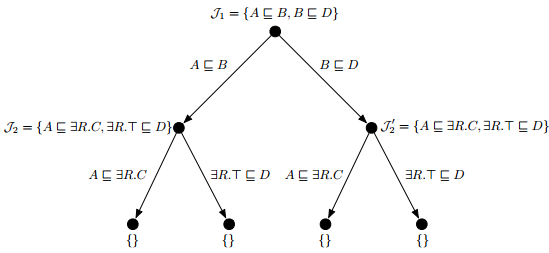
\includegraphics[width=110mm]{Figures/fig2.png}
%	\caption{Hitting Set Tree dùng để tìm kiếm giải thích \label{overflow}}
%\end{figure}
%% A foot note
%{\let\thefootnote\relax\footnotetext{*\textit{
%					$J_{1}$,$J_{2}$,$J_{2}^{'}$ được tính ra nhờ giải thuật Black-box hoặc Glass-box được đề cập ở trên.
%}}
%\hspace*{.05\textwidth} Quá trình lặp lại cho đến khi chúng ta không còn tạo được node mới nào, tại thời điểm này thì việc xây dựng HST cũng hoàn tất. \textit{Tất cả} các kiểm chứng để giả thích cho $\beta$ $\models$ $\eta$ chính là nhãn của các node trong HST. Thêm một điều nữa, là tất cả các đặc điểm đơn giản nhất để chứng minh $\beta$ $\models$ $\eta$ nằm trên các cạnh từ leaf-node tới root-node của cây.
%\\Ví dụ vừa nếu trên chỉ biểu diễn những bước cơ bản nhất để xây dựng một HST nhưng quan tâm đến bất kì khả năng tối ưu hóa nào cho giải thuật. Để đạt được một hiệu năng chấp nhận được khi ứng dụng trong thực tế thì 2 giải pháp tối ưu sẽ được nêu ra sau đây.
%				
%\paragraph{Early Path Termination} - Trong phiên bản chưa tối ưu ở trên, một node $n$ bất kì khi tạo cạnh mới với phát biểu thuộc tập $H(n)$, với $H(n)$ là tập phát biểu dán nhãn $n$, phát biểu trên cạnh mới này không được nằm trên bất kì cạnh nào nối $n$ với một node kế cận (successor nodes). Chúng ta gọi các nodes có khả năng mở rộng (tạo được cạnh mới) là \textit{open} nodes, ngược lại các leaf-nodes không có khả năng mở rộng là \textit{closed} nodes,. Để thực hiện tối ưu hóa, sẽ có trường hợp mà những nodes không phải leaf-nodes có thể được dán nhãn bởi những tập khác $\emptyset$ những vẫn sẽ được đánh dấu là \textit{closed} nodes. Trong tình huống này, đường đi từ \textit{closed} node tới root được chỉ định là \textit{early termination} - kết thúc sớm. Để phát hiện được \textit{early termination} chúng ta sẽ làm theo quy trình sau: Nếu một HST $T$ chứa một open node $v_{1}$, có đường đi $P_{1}$ tới root node, có thêm một open node $v_{2}$ cũng trong $T$, có đường tới root node là $P_{2}$. Nếu tập dán nhãn cho $P_{1}$ bằng với tập dán nhãn cho $P_{2}$ thì $v_{2}$ sẽ được đánh dấu là \textit{closed} node và không cần thiết phải mở rộng thêm nữa. Ví dụ chúng ta có ontology $O$ chứa các phát biểu sau $O=\{1, 2, 3, 4, 5\}$ và $O$ $\models$ $\alpha$
%\begin{figure}[ht!]
%	\centering
%	\begin{tikzpicture}[every tree node/.style={draw,circle},
%					level distance=1.25cm,sibling distance=1cm,
%					edge from parent path={(\tikzparentnode) -- (\tikzchildnode)}]
%					\Tree
%					[.1,2
%					\edge node[auto=right,pos=.6] {$1$};
%					[.2,3,5 
%					\edge node[auto=right,pos=.8] {$2$};
%					[.3,5 
%					\edge node[auto=right,pos=.8] {$3$};
%					[.{$\{\}$} ]
%					\edge node[auto=right,pos=.8] {$5$};
%					[.{$\{\}$} ]    	
%					]
%					\edge node[auto=left,pos=.8] {$3$};
%					[.{$\{\}$} ]
%					\edge node[auto=left,pos=.8] {$4$};
%					[.{$\{\}$} ]
%					]
%					\edge node[auto=left,pos=.6] {$2$};
%					[.1,3,4
%					\edge node[auto=right,pos=.8] {$1$};
%					[.X ]
%					\edge node[auto=left,pos=.8] {$3$};
%					[.{$\{\}$} ]
%					]
%					]
%	\end{tikzpicture}
%	\caption{Early Termination trong HST Explanation \label{overflow}}
%\end{figure}
%				
%Chúng ta bắt đầu di chuyển root node với tập $\{1,2\}$ là các phát biểu đầu tiên tìm được trong $O$ chứng minh được $O$ $\models$ $\alpha$, thực hiện tương tự các bước đã được miêu tả ở trên ta thu được node $\{3,5\}$ là các phát biểu giải thích cho $O$ $\models$ $\alpha$, tới lúc này ta có thể thấy tập chứ đường đi theo cạnh từ node $\{3,5\}$ tới root node là $P_{1}=\{2,1\}$. Nhìn về phía bên phải ta phát hiện khi mở rộng cạnh từ node $\{1,3,4\}$ ta thu được đường đi về root node là $P_{2}=\{1,2\}$, ta thấy $P_{1} \equiv P_{2}$ do vậy nên khi dán nhãn cho node kế tiếp (được đánh dâu \xmark cho \textit{closed} node) chúng ta sẽ bỏ $\{1,2\}$ khỏi $O$ để được $O^{'}=\{3,4,5\}$, sẽ có một node giống y như node $\{3,5\}$ sẽ xuất hiện lần nữa ở node kế tiếp này nên việc kết thúc ở đây là cần thiết vì chúng ta sẽ tiếp kiệm được việc kiểm tra lại $\{3,5\}$ như ở bên trái.
%				
%\paragraph{Justification Reuse} - Cách quan trọng thứ hai để tối ưu là sử dụng lại các kiểm chứng. Trong phiên bản không tối ưu sử dụng ở ví dụ ontology $\beta$ ở trên, kiểm chứng được tìm ra nhờ các giải thuật Blackbox hay Glassbox cho từng node $v$ được thêm vào cây. Kiểm chứng hay tập các phát biểu được sử dụng để dán nhãn $v$, được tính toán dựa trên $O \backslash S$, với $S$ là tập các nhãn trên đường đi từ $v$ về root node. Thay vì dùng Glassbox hay Blackbox để tính $J$ trong $O \backslash S$, chúng ta có thể làm theo cách sau: nếu HST chứa vài node khác $v^{'}$ mà được dán nhãn với kiểm chứng $J$, và $S$ không giao (có phần tử chung) với $J$ thì $J$ có thể được sử dụng làm nhãn cho $v$. Lý do là vì khi $J\subseteq$ $O$ và $S\cap J = \emptyset$ thì sẽ tồn tại trường hợp $J\subseteq O \backslash S$, từ đó $J$ được tính như một kiểm chứng cho để có thể dán nhãn $v$. Sử dụng lại các phát biểu chứng minh (hay kiểm chứng) sẽ giúp tiết kiệm nhiều lời gọi hàm không cần thiết tới Blackbox hoặc Glassbox từ đó tăng được hiệu năng.
%\\
%\paragraph{Kết luận} Tính năng vừa trình bày \textit{Tìm tất cả các giải thích cho kết quả suy luận}, kĩ thuật \textit{Axiom Pinpoint} và \textit{BlackBox} được đã được được các tác giả của bài báo \cite{matt_horridge} và \cite{axiomPinpoint}, đưa vào thư viện lập trình cho OWL-API sẽ được giới thiệu trong chương sau. Trên đây là toàn bộ những kiến thức đã tìm hiểu được mà chúng em tin rằng chúng nếu không nắm được chúng thì việc phát triển ontology và thao tác với thư viện lặp trình liên quan đến ngôn ngữ OWL sẽ gặp rất nhiều khó khắn.
%% ----------------------------------------------------------------
% Nền tảng và các thư viện lập trình sử dụng
%% ----------------------------------------------------------------
\section{Nền tảng và các thư viện lập trình sử dụng}
\textbf{Giới thiệu} Trong phần này, chúng em xin giới thiệu khái quát qua nền tảng và các thư viện lập trình (API) được sử dụng để xây dựng hệ thống. Các thư viện sử dụng gồm có OWLAPI \cite{owlapi}, SWRL-API \cite{swrlapi}, Pellet \cite{pellet} và nền tảng web sử dụng - Vaadin Framework.
\subsection{Vaadin Framework }
\paragraph{Giới thiệu} Vaadin Framework là nền tảng xây dựng một ứng dụng web trên Java được thiết kế giúp tạo ra một ứng dụng web chất lượng cao một cách dễ dàng nhất - tập trung chủ yếu vào one-page web application. Không giống như những framework web hiện nay đòi hỏi lập trình viên phải có kiến thức về HTML5, Javascript và ít nhất một ngôn ngữ back-end. Vaadin giúp chúng ta tạm quên việc đi việc phải viết các client Javascript hay từng dòng HTML để xây dựng giao diện người dùng - nói cách khác nó làm cho công việc phát triển front-end trở nên cực kì đơn giản, dễ hình dung nhất là việc phát triển một ứng dụng web trên Vaadin cũng tương tự khi chúng ta phát triển một ứng dụng desktop thông thường với các công cụ Java như AWT, Swing, hay SWT hoặc window form với C\verb|#|(C-Sharp).  Với Vaadin, để phát triển được toàn bộ một ứng dụng, ngôn ngữ duy nhất chúng ta cần nắm đó là Java. Một ví dụ minh họa về tính đơn giản trong khi sử dụng Vaadin:
\begin{verbatim}
Button button = new Button("Demo");
button.addClickListener( new ClickListener() {
layout.addComponent(new Label("The button was clicked"));
}
\end{verbatim}
Đây là kết quả:
\begin{figure}[H]
	\centering
	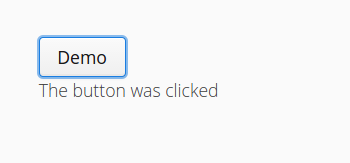
\includegraphics[width=80mm]{Figures/vaadin_democlick.png}
	\caption{Vaadin Demo Click\label{overflow}}
\end{figure}
Thử nhìn lại nếu chúng ta xây dựng cùng chức năng trên dù là thủ công hay sử dụng các framework Web thông thường thì đều cần phải có một client script đảm nhận việc bắt sự kiện click của người dùng ở browser (front-end) và truyền nó lên server, ngay khi server nhận được (phải có đoạn code ở server "back-end" để xử lý thông tin click truyền lên từ browser), server sẽ trả về thông báo "The button was clicked", rồi front-end javascript phải thêm hay chèn một đoạn text "The button was clicked" vào HTML. Với Vaadin tác vụ vừa mô tả được thực hiện bằng đoạn code trên một cách đơn giản và dễ hiểu hơn rất nhiều.
\subsubsection{Kiến trúc}
Vaadin hỗ trợ 2 mô hình lập trình: client và server. Mô hình lập trình phía server mạnh mẽ hơn. Mô hình lập trình phía server đảm nhận phần giao diện trên trình duyệt và giao tiếp AJAX giữa trình duyệt và server - hay nói cách khác các giao tiếp giữa server-client nhằm hỗ trợ những thao tác của người dùng đã được xử lý bởi framework và được cài đặt vào bên trong các \textit{Component} của Vaadin. Trong phạm vi ứng dụng mà chúng em xây dựng chỉ sử dụng những thành phần server - chỉ sử dụng các \textit{Component} mà Vaadin cung cấp, cộng với một vài plugin (được viết sẵn cho Vaadin) từ Vaadin Directory \cite{vaadindirectory} để giúp việc phát triển nhanh chóng hơn. 
%\\
%Hình sau mô tả kiến trúc cơ bản của một ứng dụng web trên Vaadin Framework. Kiến trúc ứng dụng phía server bao gồm nền tảng server (Server-side framework) và hệ thống phía client (Client-side engine). 
%\begin{figure}[ht!]
%	\centering
%	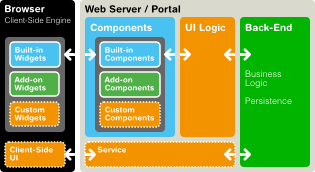
\includegraphics[width=80mm]{Figures/vaadin_architecture0.png}
%	\caption{Kiến trúc của Vaadin\label{overflow}}
%\end{figure}

\paragraph{Web Server} gồm các thành phần:
\begin{description}
	\item[Components] Các \textit{Built-in Components}, \textit{Add-on Components} đều là những thành phần được xây dựng sẵn bởi Vaadin hoặc được cung cấp dưới dạng các add-on từ Vaadin Directory \cite{vaadindirectory} nhằm giúp việc phát triển UI nhanh chóng hơn. Chúng đảm nhiệm back-end code để giao tiếp với các \textit{Built-in Widgets}, \textit{Add-on Widgets} ở phía browser (client side).
	\item[UI Logic, Service và Custom Components] là những phần mà lập trình viên phải tự viết code để cài đặt các tác vụ tương tác mà họ mong muốn, tuy nhiên Vaadin cũng cung cấp các abstract class, interface để hỗ trợ việc này. 
	\item[Back-end] Trong một ứng dụng thông thường thì đây chính là nơi để xử lý giao tiếp với các đối tượng trong cơ sở dữ liệu - nơi thực hiện các thao tác Create Read Update Delete (CRUD) \cite{vaadinarchitecture}.
\end{description}
\paragraph{Client-Side Engine} gồm các thành phần:
\begin{description}
	\item[Built-in Widgets] Đây chính là thành phần Client-side của \textit{Built-in Components} đảm nhiệm bắt các sự kiện của người dùng với browser và giao tiếp với các \textit{Built-in Components} ở server.
	\item[Add-on Widgets] là client-side của \textit{Add-on Components}.
	\item[Custom-Widgets] là client-side của \textit{Custom Components}.
\end{description}
%Toàn bộ các thành phần ở Client-side Engine đều được xây dựng bằng JavaScript. Đây là một ưu thế so với các nền tảng trên Flash, Java Applets hay các plugins khác. Vaadin dựa trên sự hỗ trợ của Google Web Toolkit cho nhiều trình duyệt khác nhau, nên lập trình viên không cần lo lắng về sự tương thích của các trình duyệt cho ứng dụng của mình.
%\\
%Như đã nói ở trên, không giống với các framework web khác là tách biệt front-end và back-end thành 2 phần riêng biệt, Vaadin làm điều ngược lại đó là đem cả hai thành phần đó tích hợp vào \textit{Vaadin Components}, ở hình trên chúng ta sẽ thấy một \textit{Vaadin Component} sẽ gồm một \textit{Widget} ở client-side  và một \textit{Component} tương ứng ở server side. Phân tích ví dụ Demo Click ở bên trên :
%\begin{itemize}
%	\item \textbf{Vaadin Component} chính là một Vaadin Component.
%	\item \textbf{UILogic} chính là \textit{layout.addComponent(new Label("The button was clicked"));}
%\end{itemize}

Tóm lại, Vaadin cung cấp sẵn gần như đầy đủ mọi thành phần UI chúng ta cần để phát triển một ứng dụng web tương tác tốt với người dùng một cách nhanh chóng và tiện lợi. Chúng ta sẽ giảm bớt được công việc khi phải viết Javascript, HTML cho cliend-side khi sử dụng các Vaadin UI Components.
\\
Tuy là tích hợp mọi thứ vào UI components của mình, Vaadin tách biệt UI Logic với các thiết kế giao diện. Điều này đồng nghĩa bên cạnh một giao diện mặc định rất tốt của Vaadin chúng ta có thể thiết kế giao diện một cách dễ dàng thông qua các file CSS hoặc cũng có thể tự định nghĩa HTML Template cho riêng mình \textsuperscript{*}. 
{\let\thefootnote\relax\footnotetext{*\textit{
			Vaadin Theme: https://vaadin.com/book/-/page/themes.html}}
}
\subsection{Spring Boot}
Spring Boot \cite{springboot} là một dự án nằm trong bộ \textit{Spring Application Framework} với mục đích giúp người mới sử dụng \textit{Spring} có thể dễ dàng phát triển một ứng dụng một cách nhanh nhất có thể mà không cần phải mất thời gian cấu hình trong các tập tin XML truyền thống.
\subsection{Spring 4 Vaadin}
Đây là một dự án mã nguồn mở \cite{spring4vaadin} vừa được khởi động sử dụng với nền tảng là \textit{Spring Boot} và \textit{Vaadin}, mục tiêu của dự án này là đem các thư viện mạnh mẽ của Spring Framework như Spring Data, Spring Security và đặc biệt là khả năng dependency injection vào Vaadin. Chúng em chủ yếu sử dụng các dự án này vào việc khởi tạo ứng dụng, khởi tạo các Bean Component một lần vào đưa nó (inject) vào lớp \textbf{UI} của hệ thống.
%%
\subsection{Thư viện lập trình OWLAPI}
Thư viện lập trình Ontology Web Language là một thư viện mã nguồn mở (phát hành dưới 2 giấy phép \textbf{LGPL} và \textbf{Apache}) \cite{owlapi} được viết bằng Java với mục đích hỗ trợ các lập trình viên phát triển các ứng dụng có liên quan đến OWL 2 Ontology. Tính đến thời điểm hiện tại thư viện đã được phát triển đến phiên bản 4.0 - cũng là phiên bản được sử dụng trong ứng dụng của chúng em.
Thư viện có các thành phần chính như sau: 
\begin{itemize}
	\item API để tương tác với các thành phần của OWL 2 được đề cập trong chương 2.
	\item Renderer và Parser (dùng đọc và ghi OWL 2 Ontology) nhiều dạng cú pháp khác nhau đã đề cập ở chương 2 như \textit{RDF/XML}, \textit{OWL/XML}, \textit{OWL Functional Syntax}, \textit{Manchester OWL Syntax} và \textit{Turtle}.
	\item Reasoner Interfaces hỗ trợ các loại reasoners khác nhau nhằm phục vụ cho việc suy luận.
\end{itemize}
Danh sách các Ontology Reasoner được hỗ trợ trong phiên bản 4.0: FaCT++, Hermit, Pellet \cite{pellet}, JFact.
Các đối thành phần (thực thể, mô tả lớp/thuộc tính,...) được giải thích trong lúc giới thiệu OWL 2 đều đươc OWL-API mô hình hóa thành các đối trượng trong Java, với tiếp đầu ngữ \textit{OWL} + tên thành phần. Ví dụ:
\begin{verbatim}
Class              -> OWLClass  #Lớp
ObjectProperty     -> OWLObjectProperty # thuộc tính đối tượng
OWLClassExpression -> OWLClassExpression # Mô tả lớp
\end{verbatim} 
Tương tự cho các thành phần OWL 2 khác.
\subsection{Pellet Reasoner}
Như đã đươc nhắc đến nhiều lần trong báo cáo, suy luận được xem là một điểm đáng giá nhất của ngôn ngữ OWL2. Tuy nhiên, việc suy luận ra các phát biểu hàm ý rõ ràng không phải là một việc dễ dàng nếu chúng ta thực hiện thủ công bằng cách đọc và hiểu các phát biểu như đã làm trong chương 2. Sử dụng Reasoner sẽ làm cho công việc suy ra các mảnh thông tin ẩn chứa bên trong Ontology trở nên dễ dàng hơn rất nhiều, có rất nhiều reasoner được phát triển để thực hiện tác vụ này. Trong số đó Pellet \cite{pellet} là một thư viện tối ưu nhất và một ưu điểm đặc biệt là khả năng suy luận từ những SWRL Rule. Pellet có thể được sử dụng với OWL-API thông qua reasoner Interface của OWL-API.
\begin{verbatim}
OWLReasonerFactory rf; // OWLReasoner là inteface reasoner của OWL-API
OWLReasonerFactory rf = PelletReasonerFactory.getInstance();
OWLReasoner rs = rf.createReasoner(ontology, new SimpleConfiguration());
\end{verbatim}
\subsection{SWRL API}
SWRL API được xây dựng bởi nhóm phát triển dự án Protege \cite{protege} với mục tiêu tổ chức các SWRL Rule theo tên nhằm dễ dàng quản lý, đồng thời họ cũng giới thiệu SQWRL \cite{swrlapi} một ngôn ngữ truy vấn dành cho Ontology. Trong nội dung báo cáo, chúng em chỉ sử dụng tính năng SWRL Rule của SWRLAPI, các tính năng còn lại có thể được tham khảo tại \cite{swrlapi}. Các tính năng mà chúng em sử dụng gồm render, parse SWRL Rule và thêm/xóa SWRL Rule theo tên của chúng. Một ví dụ nhanh về cách sử dụng API này với OWL-API:
\begin{verbatim}
OWLOntology ont = // load ontology ../
// Convert OWLOntology -> SWRLAPIOWLOntology
SWRLAPIOWLOntology SWRLOnt =  SWRLAPIFactory.createOntology(ont);
\end{verbatim}


\chapter{Thiết kế hệ thống phân loại tự động}
\paragraph{Giới thiệu} Vè nội dung chương này, chúng em sẽ miêu tả lại quá trình mà chúng em đã thiết kế nên hệ thống gồm các bước như cách áp dụng một số design pattern vào việc xây dựng hệ thống, các phác thảo sơ khai của giao diện, cách kết hợp các thư viện lập trình đã giới thiệu với Vaadin Framework và cuối cùng là thiết kế một ontology dùng để trình bày tính năng phân loại sau khi hệ thống được xây dựng thành công.
\section{Giải thích về việc lựa chọn nền tảng sử dụng}
Như đã được trình bày ở mục trên, Vaadin Framework là một nền tảng xây dựng Web dựa trên ngôn ngữ Java, nhưng không giống với phần lớn các framework Web khác vốn hoạt động theo mô hình Model-View-Controller (MVC). Vaadin chỉ cung cấp một bộ gồm rất nhiều UI Component có sẵn (đã được giải thích ở mục trước) làm cho việc xây dựng giao diện được đơn giản hóa một cách tối đa. Vì thế, lập trình viên sẽ không cần phải quan tâm nhiều đến HTML, JavaScript và ít phải quan tâm đến CSS, điều này giúp tập trung vào việc xây dựng logic của hệ thống tốt hơn. Việc thiết kế cho hệ thống này trên nền web sẽ tương tự như khi thiết kế một ứng dụng GUI trên nên Desktop nhờ có Vaadin.
\section{Thiết kế Use Case của hệ thống}
Trước tiên, chúng em giới thiệu một cách tổng quan về cách hệ thống hoạt động.
 \begin{figure}[ht!]
 	\centering
 	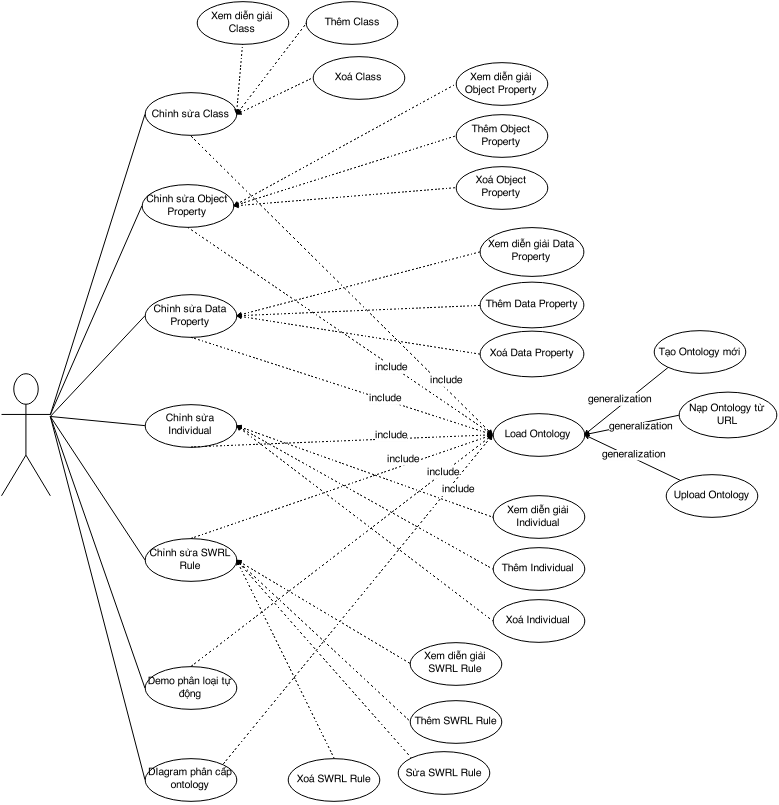
\includegraphics[width=155mm,height=170mm]{Figures/usecase.png}
 	\caption{Sơ đồ Use Case của hệ thống \label{overflow}}
 \end{figure}
\section{Thiết kế giao diện phác thảo}
Hệ thống hay ứng dụng sẽ gồm 2 view chính: view đầu tiên tạm gọi là EntryView dùng để nạp/tạo mới các tài liệu OWL 2. View thứ hai chính là view chính của ứng dụng gọi làm MainView cho phép thực hiện việc chỉnh sửa ontology, thực hiện suy luận (phục vụ cho tính năng phân loại). 
\begin{figure}[ht!]
	\centering
	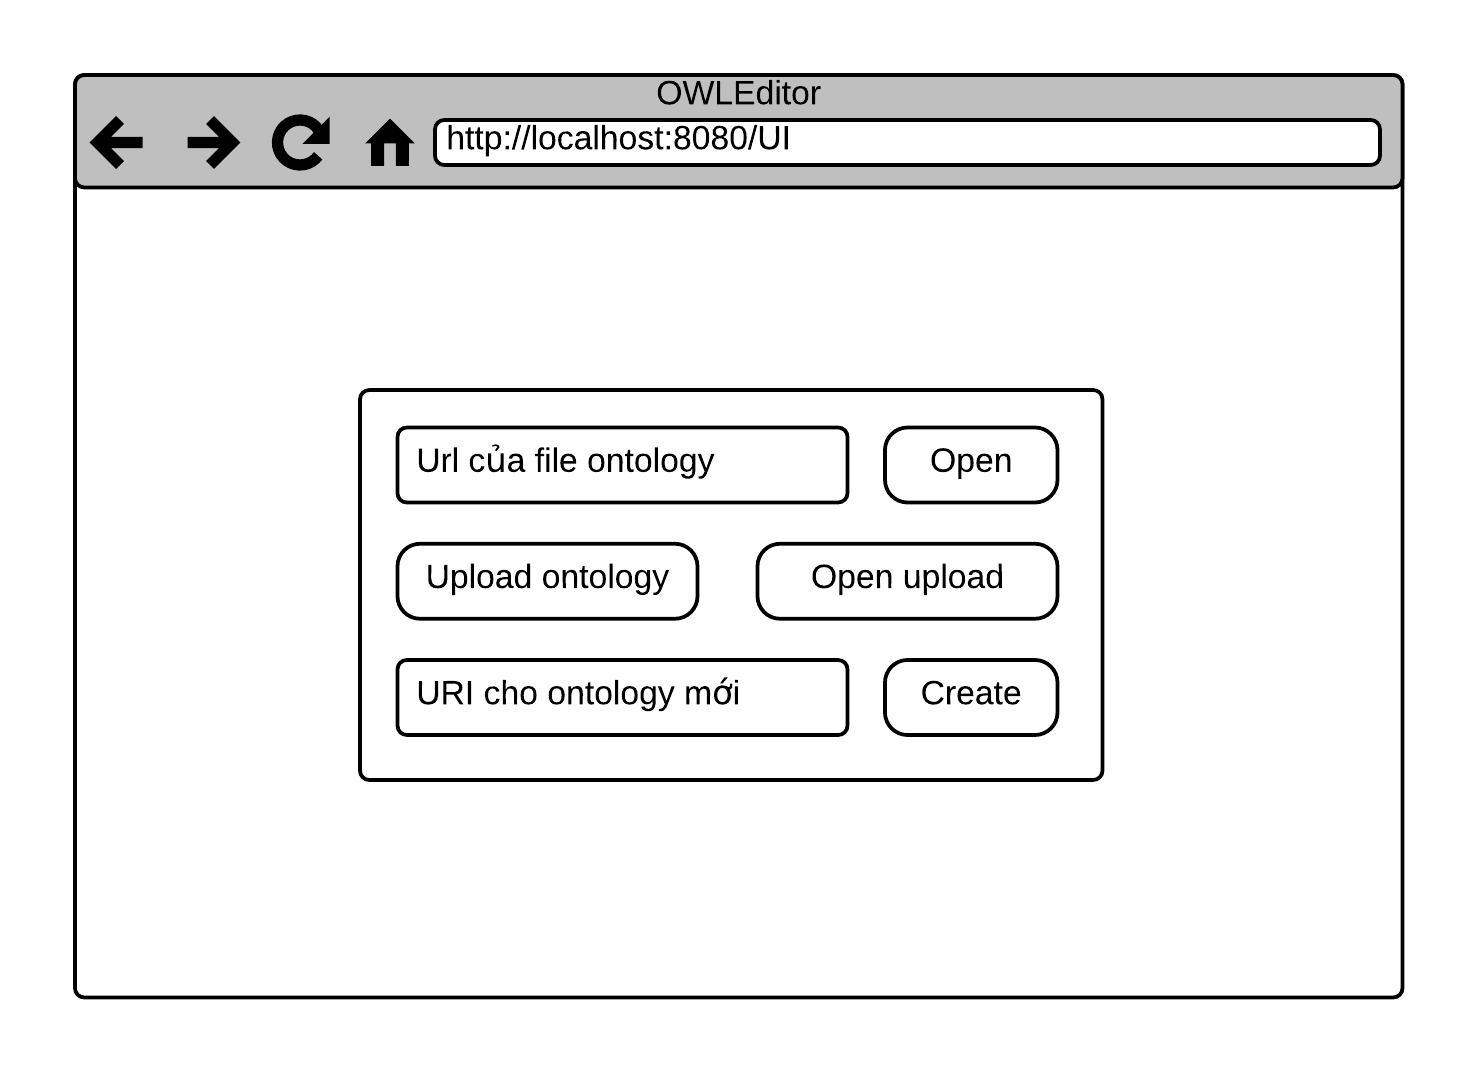
\includegraphics[width=150mm,height=95mm]{Figures/ui_entryview.png}
	\caption{Phác thảo Entry View \label{overflow}}
\end{figure}
MainView sẽ gồm nhiều tab, mỗi loại thực thể (gồm lớp, thuộc tính đối tượng, thuộc tính dữ liệu, cá thể) và SWRL Rule sẽ được tổ chức thành từng tab với tên tương ứng. 
\begin{figure}[h!]
	\centering
	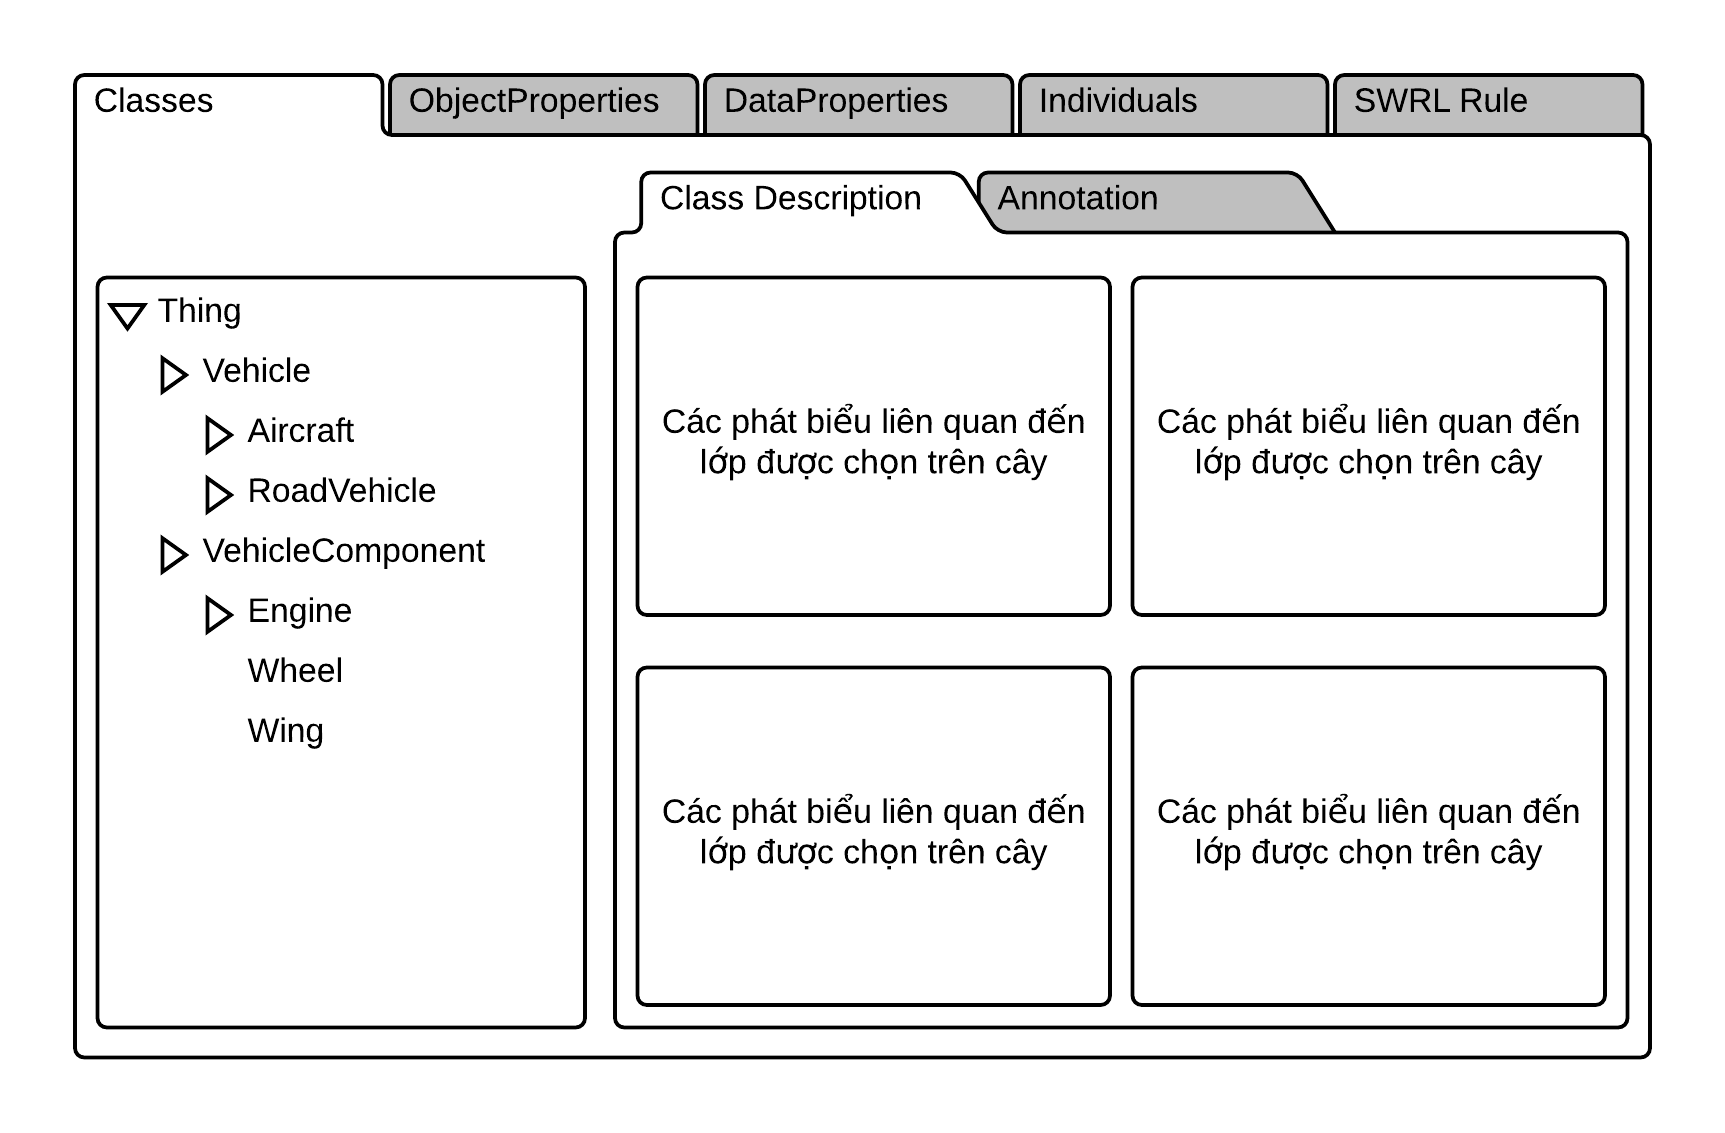
\includegraphics[width=150mm,height=95mm]{Figures/ui_mainview.png}
	\caption{Phác thảo Main View - Tab "Classes" (chứa lớp và các mô tả lớp liên quan) \label{overflow}}
\end{figure}
\begin{figure}[h!]
	\centering
	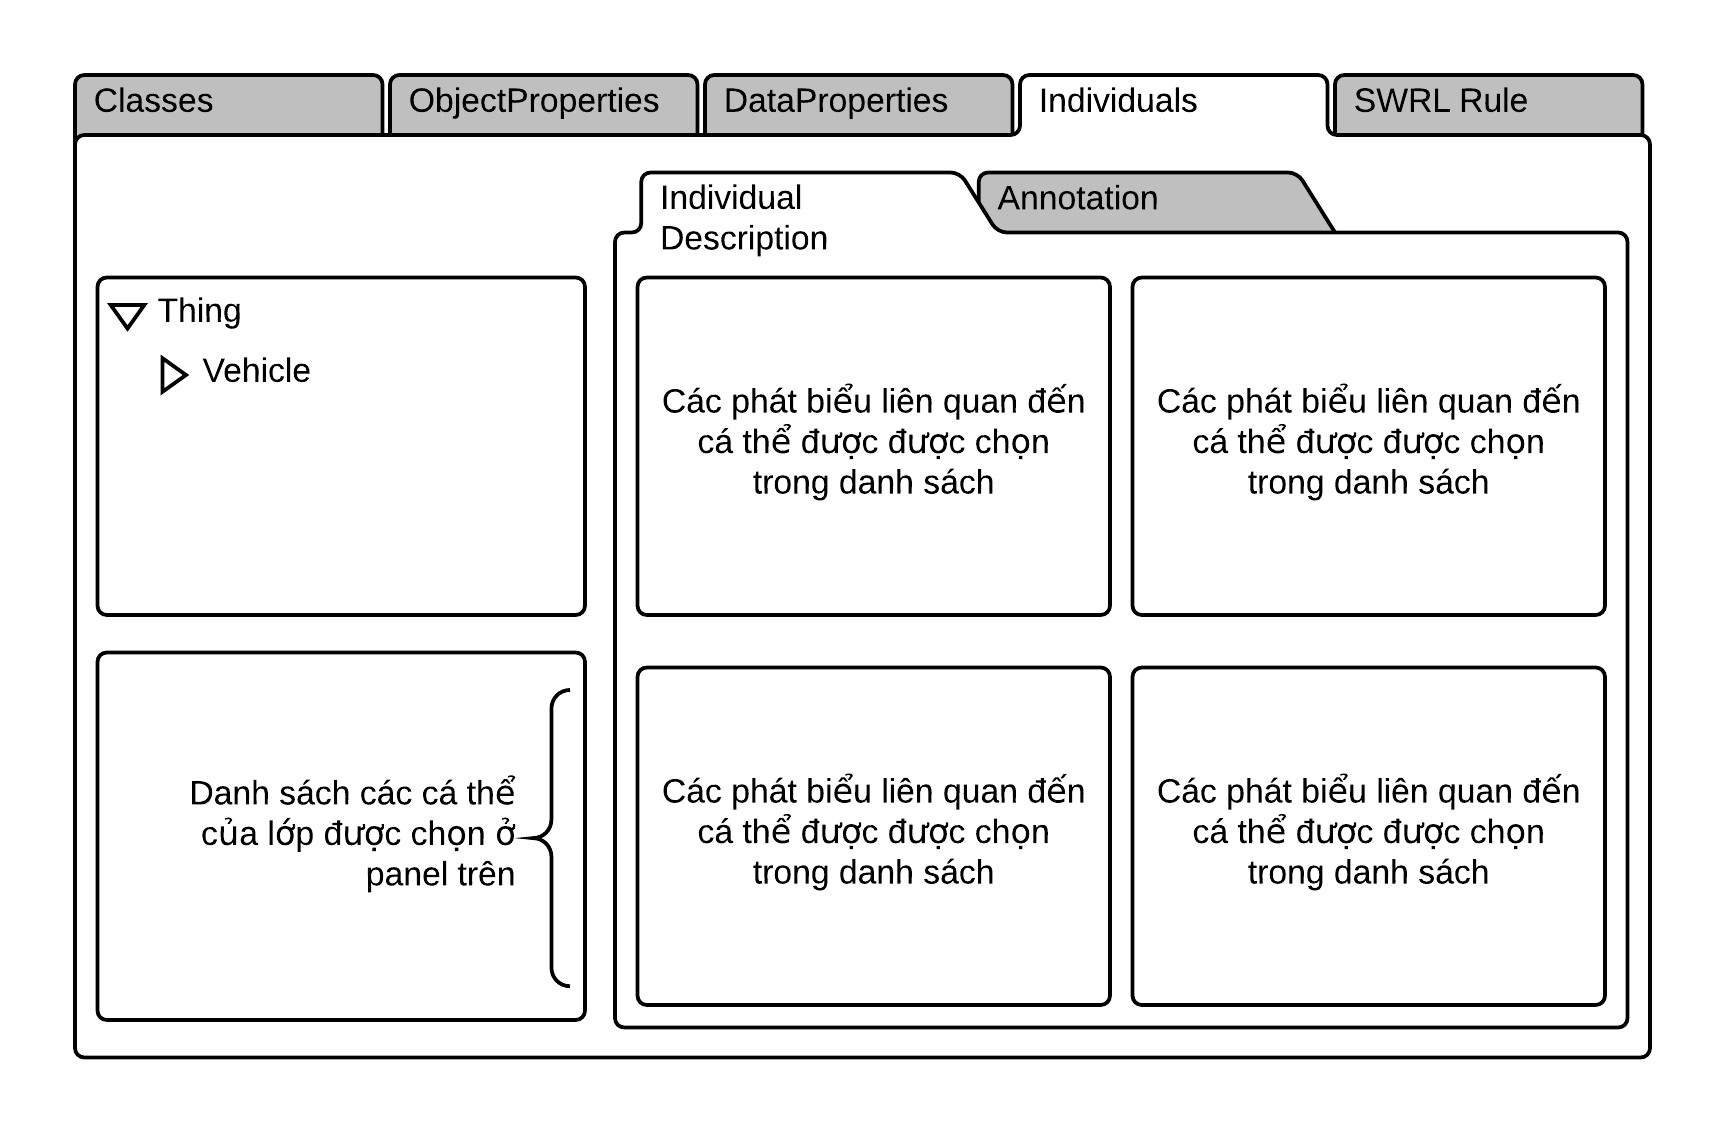
\includegraphics[width=150mm,height=95mm]{Figures/ui_mainview_individual.png}
	\caption{Phác thảo Main View - Tab "Individuals" (chứa cá thể và các mô tả liên quan) \label{overflow}}
\end{figure}
\begin{figure}[h!]
	\centering
	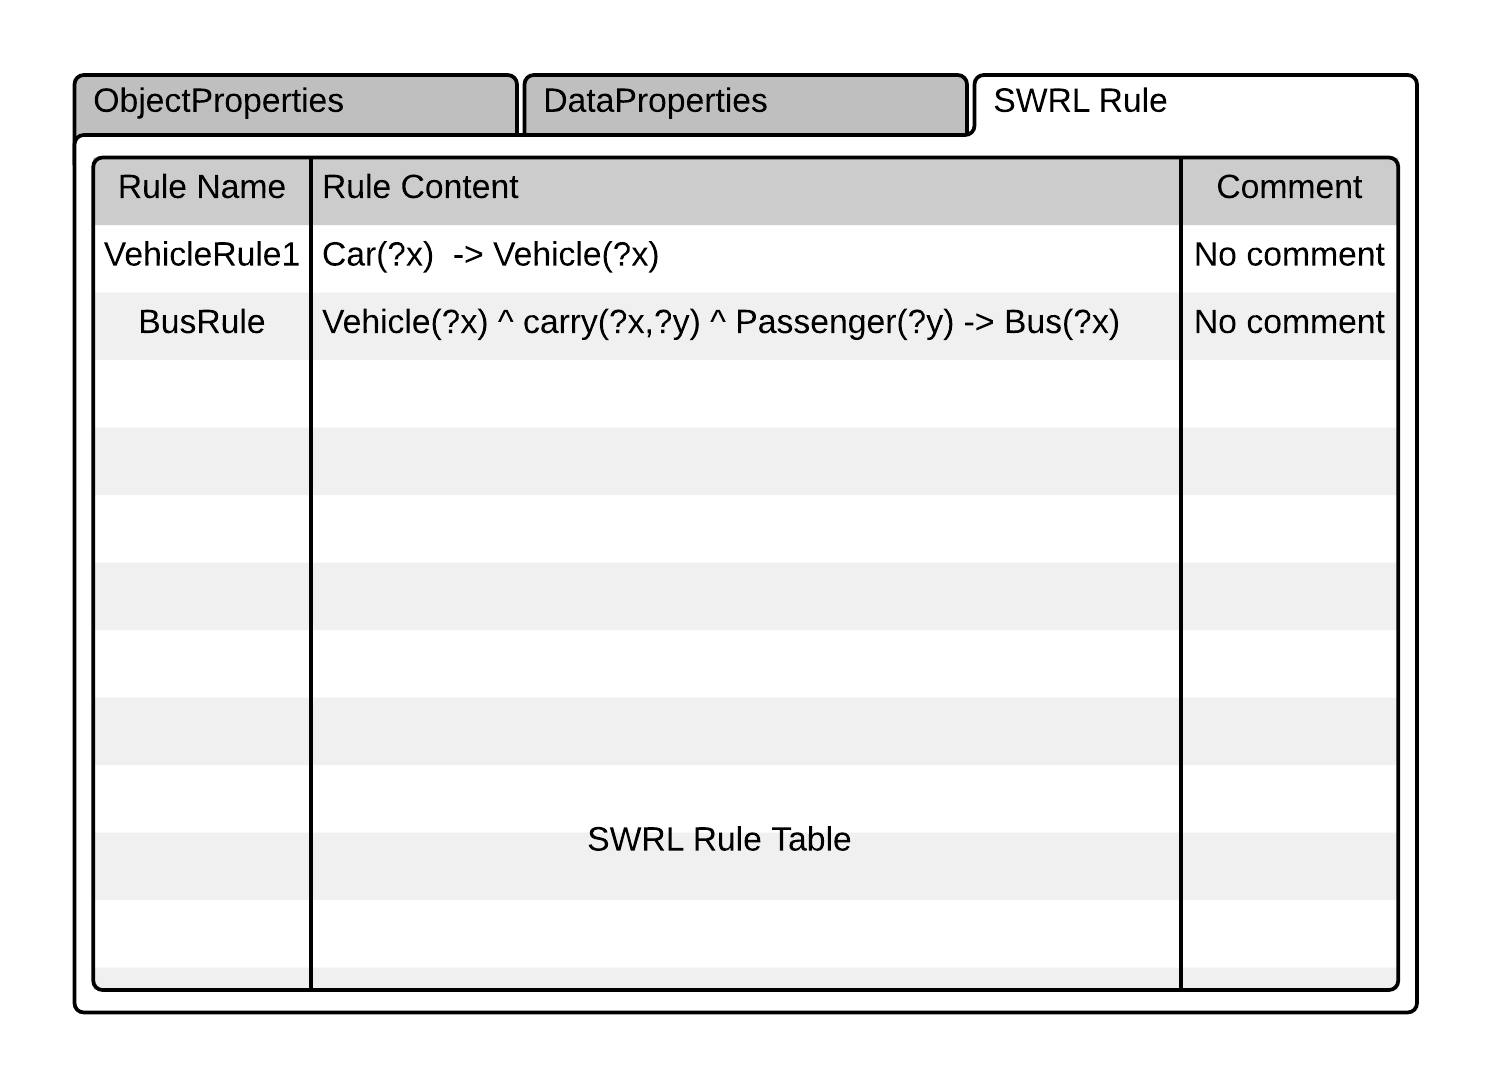
\includegraphics[width=150mm,height=95mm]{Figures/ui_mainview_swrltab.png}
	\caption{Phác thảo Main View - Tab "SWRL Rules" \label{overflow}}
\end{figure}
Các tab về lớp (Class), thuộc tính đối tượng (Object Propery) và thuộc tính dữ liệu (Data Propery) sẽ có bố cục giống nhau (Hình 3.3). Bên trái là một cây biểu diễn cấu trúc phân cấp của các loại thực thể này và bên phải là các panel nhỏ. Từng panel sẽ tương ứng với từng loại phát biểu có liên quan đến thực thể được chọn bên trái. Riêng tab về các cá thể sẽ có bố cục hơi khác so với các thực thể còn lại, nó sẽ có thêm một danh sách (sẽ nằm bên dưới cấu trúc cây chứa các lớp - Hình 3.4). Bên trong tab SWRL Rules sẽ là một bảng gồm chứa các rule, chia thành 3 cột gồm tên, nội dung và lời chú thích cho rule (Hình 3.5).
\begin{figure}[h!]
	\centering
	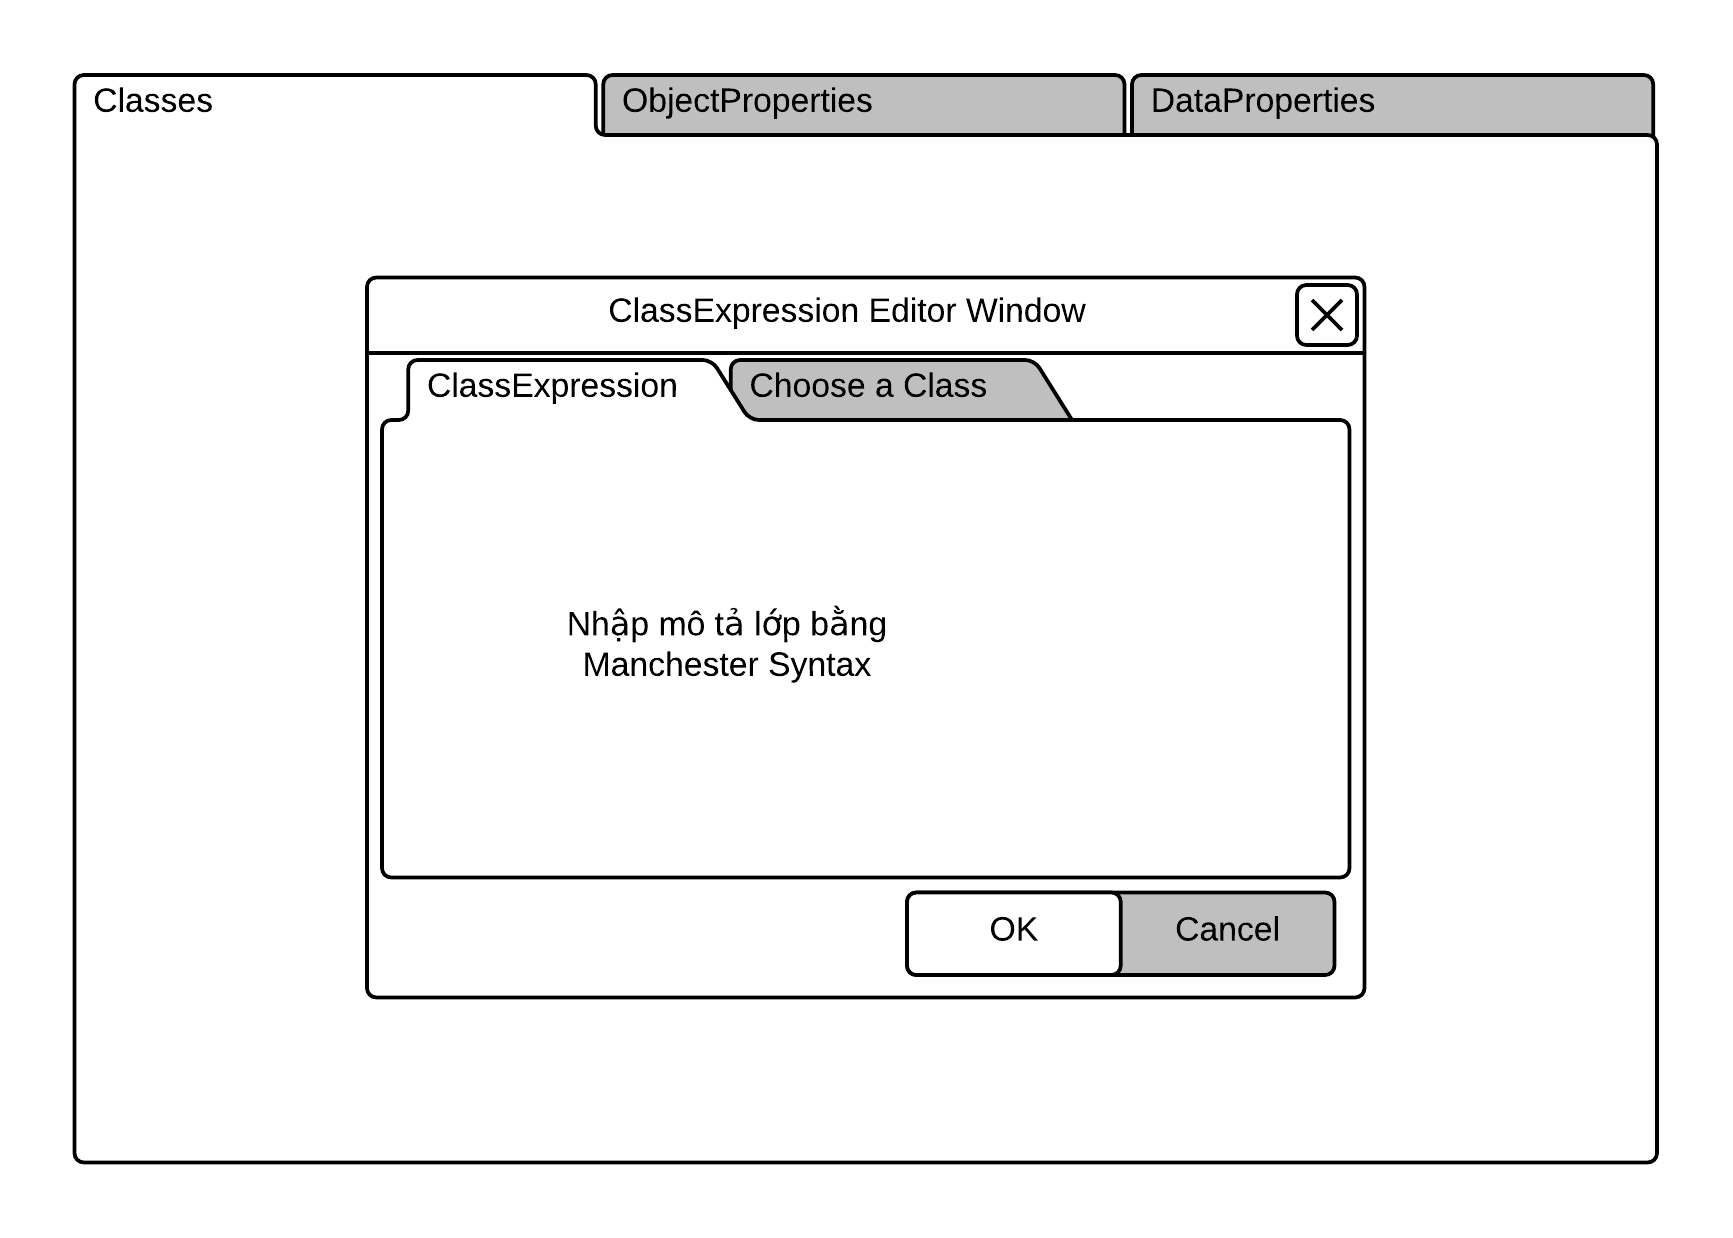
\includegraphics[width=150mm,height=100mm]{Figures/ui_classexpressioneditor.png}
	\caption{Phác thảo cửa sổ biên tập mô tả lớp\label{overflow}}
\end{figure}
\begin{figure}[h!]
	\centering
	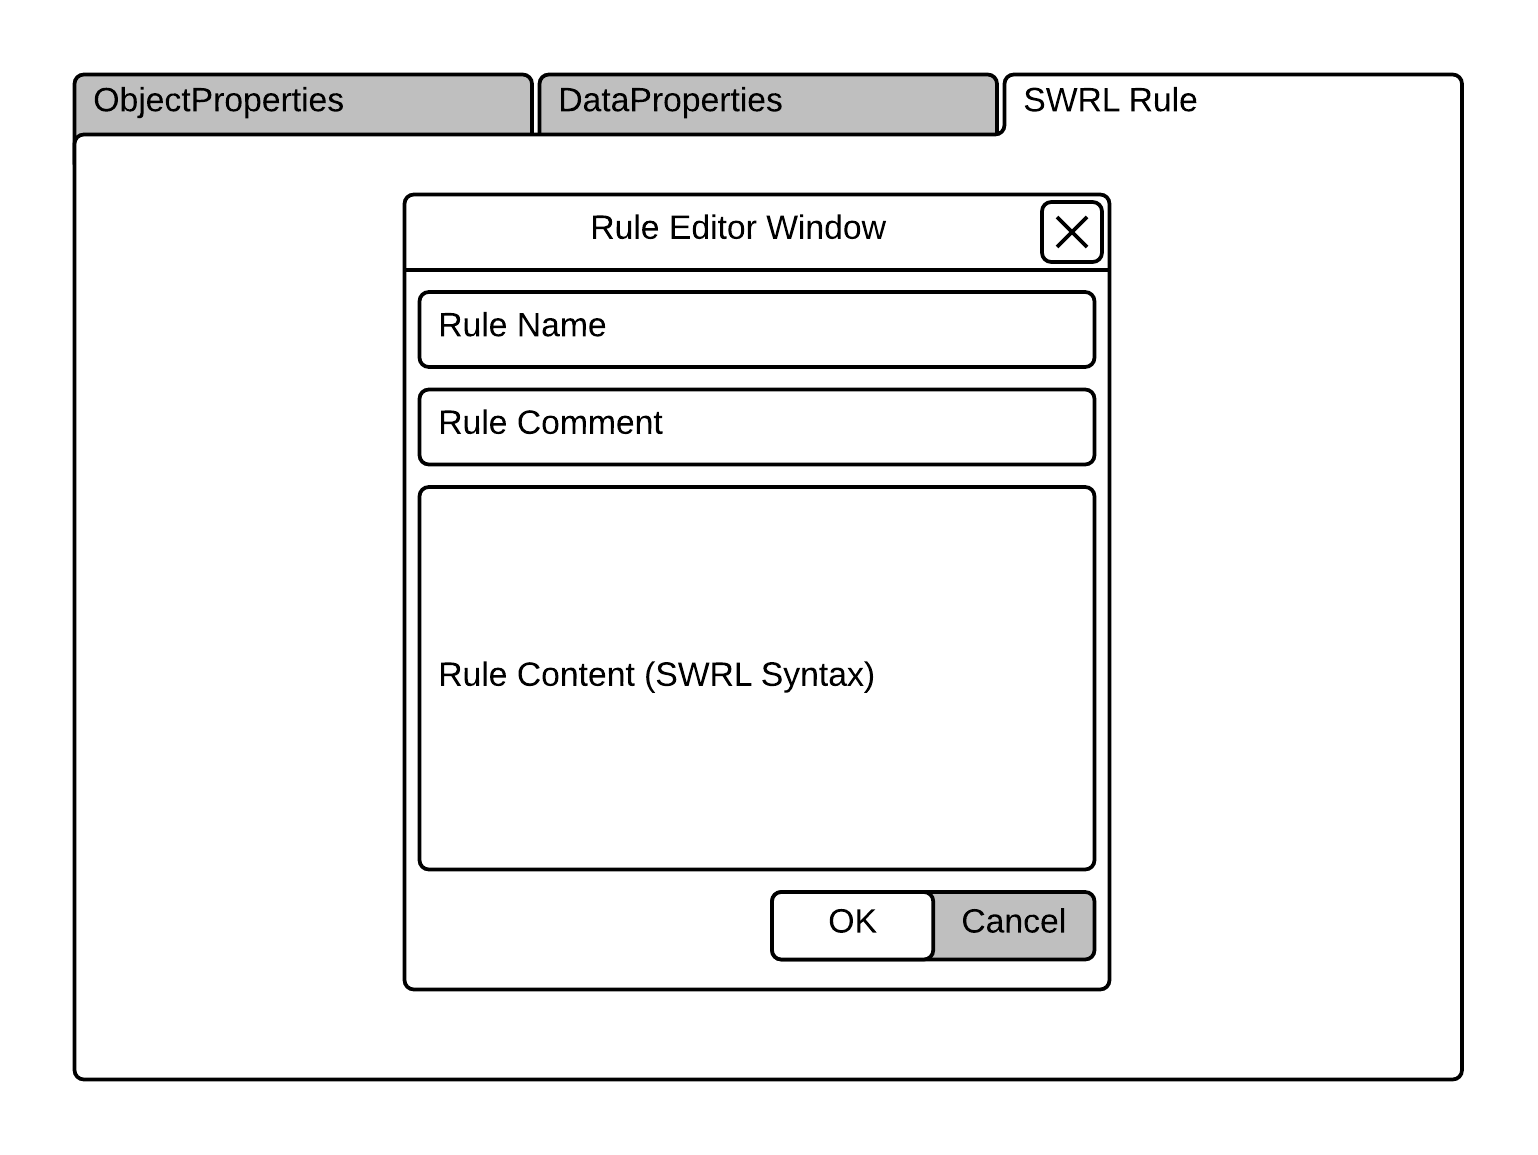
\includegraphics[width=155mm,height=95mm]{Figures/ui_mainview_ruleeditor.png}
	\caption{Phác thảo cửa sổ biên tập rule \label{overflow}}
\end{figure}
Ngoài các view và tab đã kể ở trên, thì ứng dụng buộc phải có thêm các thành phần giao diện hỗ trợ viêc biên tập mô tả lớp, thuộc tính, cá thể (class/property expression, individual assertion axiom) và việc biên tập SWRL Rule. Các hình 3.6, 3.7  thể hiện phác thảo về các giao diện đảm nhiệm những tính năng vừa nêu.
\section{Truy xuất đến các thành phần của Ontology trong OWL-API bằng cách áp dụng Visitor Pattern}
Trong OWL-API, các đối tượng dữ liệu có cấu trúc tương tự với các thành phần trong OWL 2 Ontology (được trình bày trong mục 2.2.3) - tên của các đối tượng dữ liệu sẽ có thêm tiếp đầu ngữ \textit{"OWL"} cộng với tên của thành phần trong OWL 2 như \textit{Ontology} thì đối tượng trong OWL-API sẽ là \textit{OWLOntology}, \textit{ClassExpression} (mô tả lớp) thì đối tượng tương ứng là \textit{OWLClassExpression}, tương tự cho các thành phần khác. Việc tương tác và thay đổi sẽ diễn ra trong đối tượng \textit{OWLOntology} - đối tượng Java biểu diễn một OWL 2 ontology. 
\\
Như đã được giới thiệu trong mục 2.2.3, với một cấu trúc phức tạp gồm nhiều đối tượng được mở rộng và thừa kế từ các loại đối tượng khác, thì việc truy xuất đến từng thành phần cụ thể và áp dụng các thay đổi khác nhau lên chúng là một tác vụ khó nếu không áp dụng Visitor Pattern.
\subsection{Visitor Pattern}
\begin{figure}[h!]
	\centering
	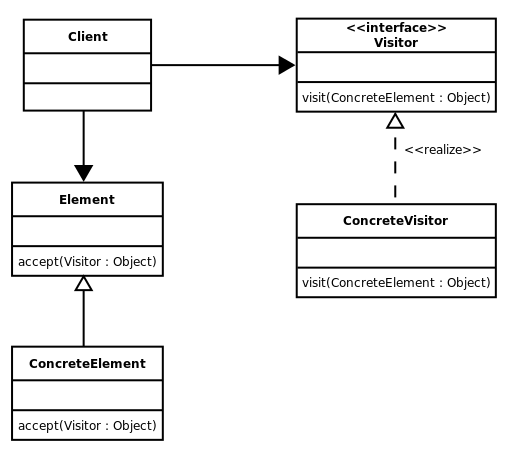
\includegraphics[width=100mm]{Figures/visitor_diagram.png}
	\caption{Visitor Design Pattern\label{overflow}}
\end{figure}
Visitor Pattern là một design pattern trong lập trình hướng đối tượng với mục tiêu tách biệt các cấu trúc dữ liệu khỏi giải thuật. Nói cách khác chúng ta dễ dàng thay đổi các giải thuật mong muốn lên các thành phần của OWLOntology mà không cần phải thay đổi cấu trúc của chúng. Như biểu diễn trong hình mọi loại đối tượng kế thừa/mở rộng từ IElement đều có khả năng truy xuất bởi các đối tượng áp dụng Interface Visitor, các giải thuật mong muốn sẽ được định nghĩa trong phương thức \textit{visit}.
\subsection{Visitor trong OWL-API}
Trong OWL-API cung cấp sẵn một số các Interface Visitor cho từng loại thành phần cụ thể. Ví dụ như OWLClassExpression sẽ có OWLClassExpressionVisitor, hay OWLDatatype sẽ có OWLDatatypeVisitor, .v.v.. . Hình sau đây miêu tả cách hoạt động của OWLClassExpressionVistor.
\begin{figure}[h!]
	\centering
	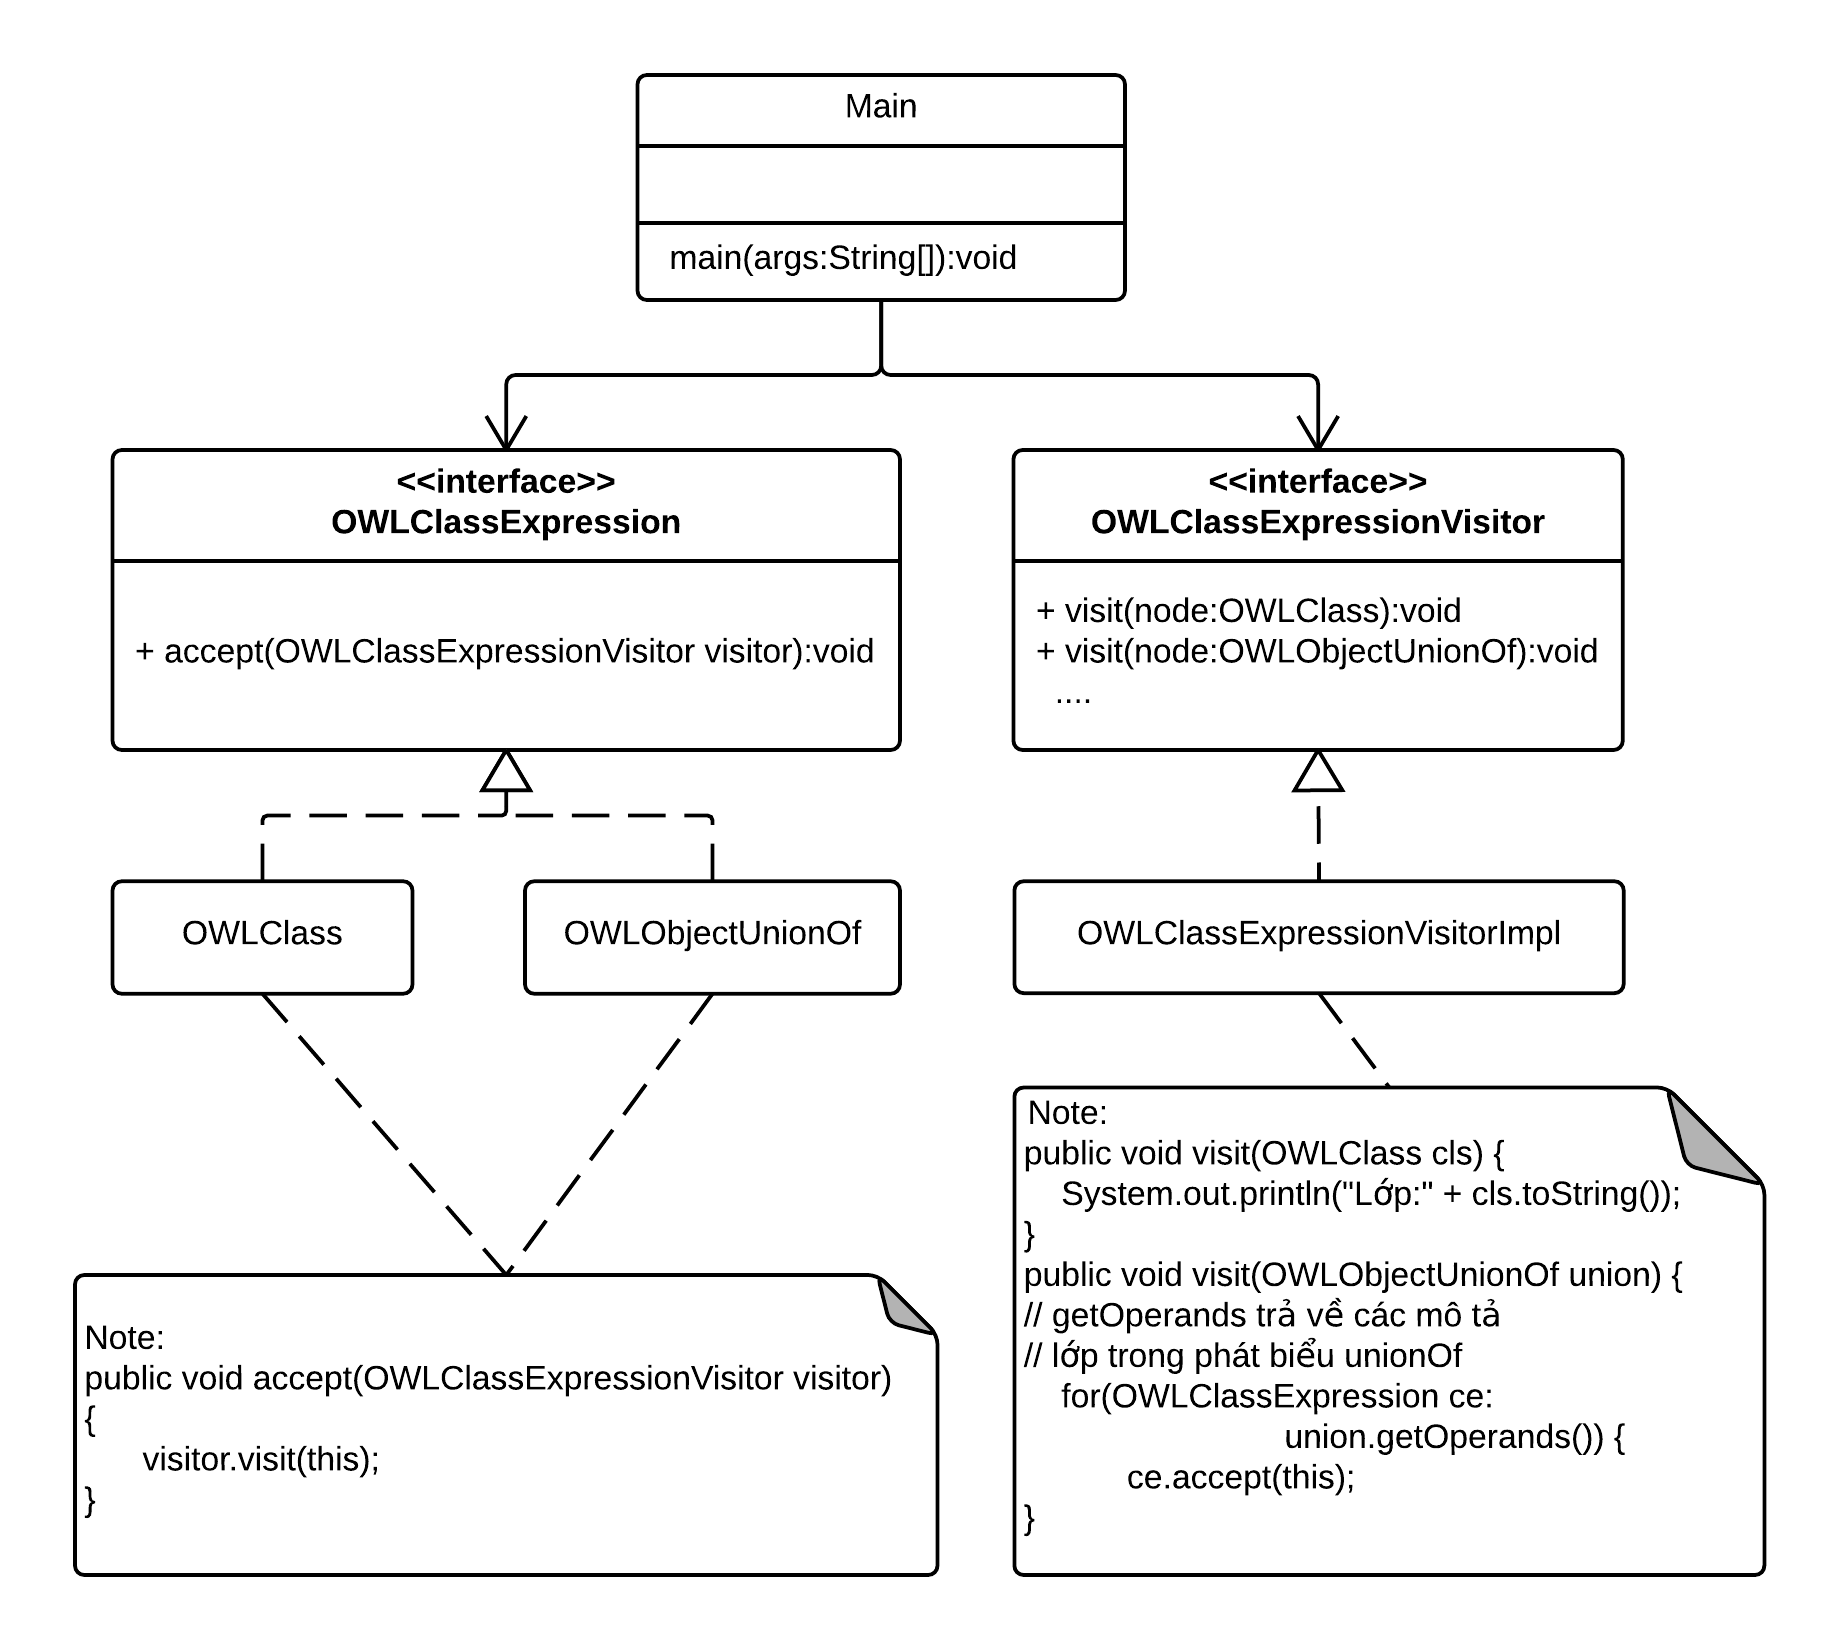
\includegraphics[width=145mm]{Figures/uml_classdiagram_classexpressionvistior_nobackground.png}
	\caption{OWLClassExpressionVisitor trong OWL-API \label{overflow}}
\end{figure}
{\let\thefootnote\relax\footnotetext{*\textit{
		OWLDataFactory: nằm trong OWL-API với chức năng dùng như một nhà máy tạo ra mọi loại đối tượng từ lớp, thuộc tính tới các phát biểu.
}}
Giải sử chúng ta có một mô tả lớp (class expression) bằng Manchester Syntax \textit{"Car and Bike"} và hàm main trong hình khai báo như sau:
\begin{verbatim}
// void main 
OWLDataFactory factory = OWLManager.getOWLDataFactory();
OWLClass car = factory.getOWLClass("a:Car");
OWLClass bike = factory.getOWLClass("a:Bike");
OWLObjectUnionOf union = factory.getOWLObjectUnionOf(car, bike);
OWLClassExpressionVisitor visitor = new OWLClassExpressionVisitorImpl();
union.accept(visitor);
// Ta sẽ có output là 
Lớp: a:Car
Lớp: a:Bike                                       
\end{verbatim}
Visitor lớn nhất trong OWL-API là \textit{OWLObjectVisitor} có khả năng truy vấn đến tất cả các loại đối tượng thuộc \textit{OWLOntology}. Visitor này thực ra được tập hợp lại từ nhiều visitor nhỏ hơn (Hình 3.10).
\begin{figure}[h!]
	\centering
	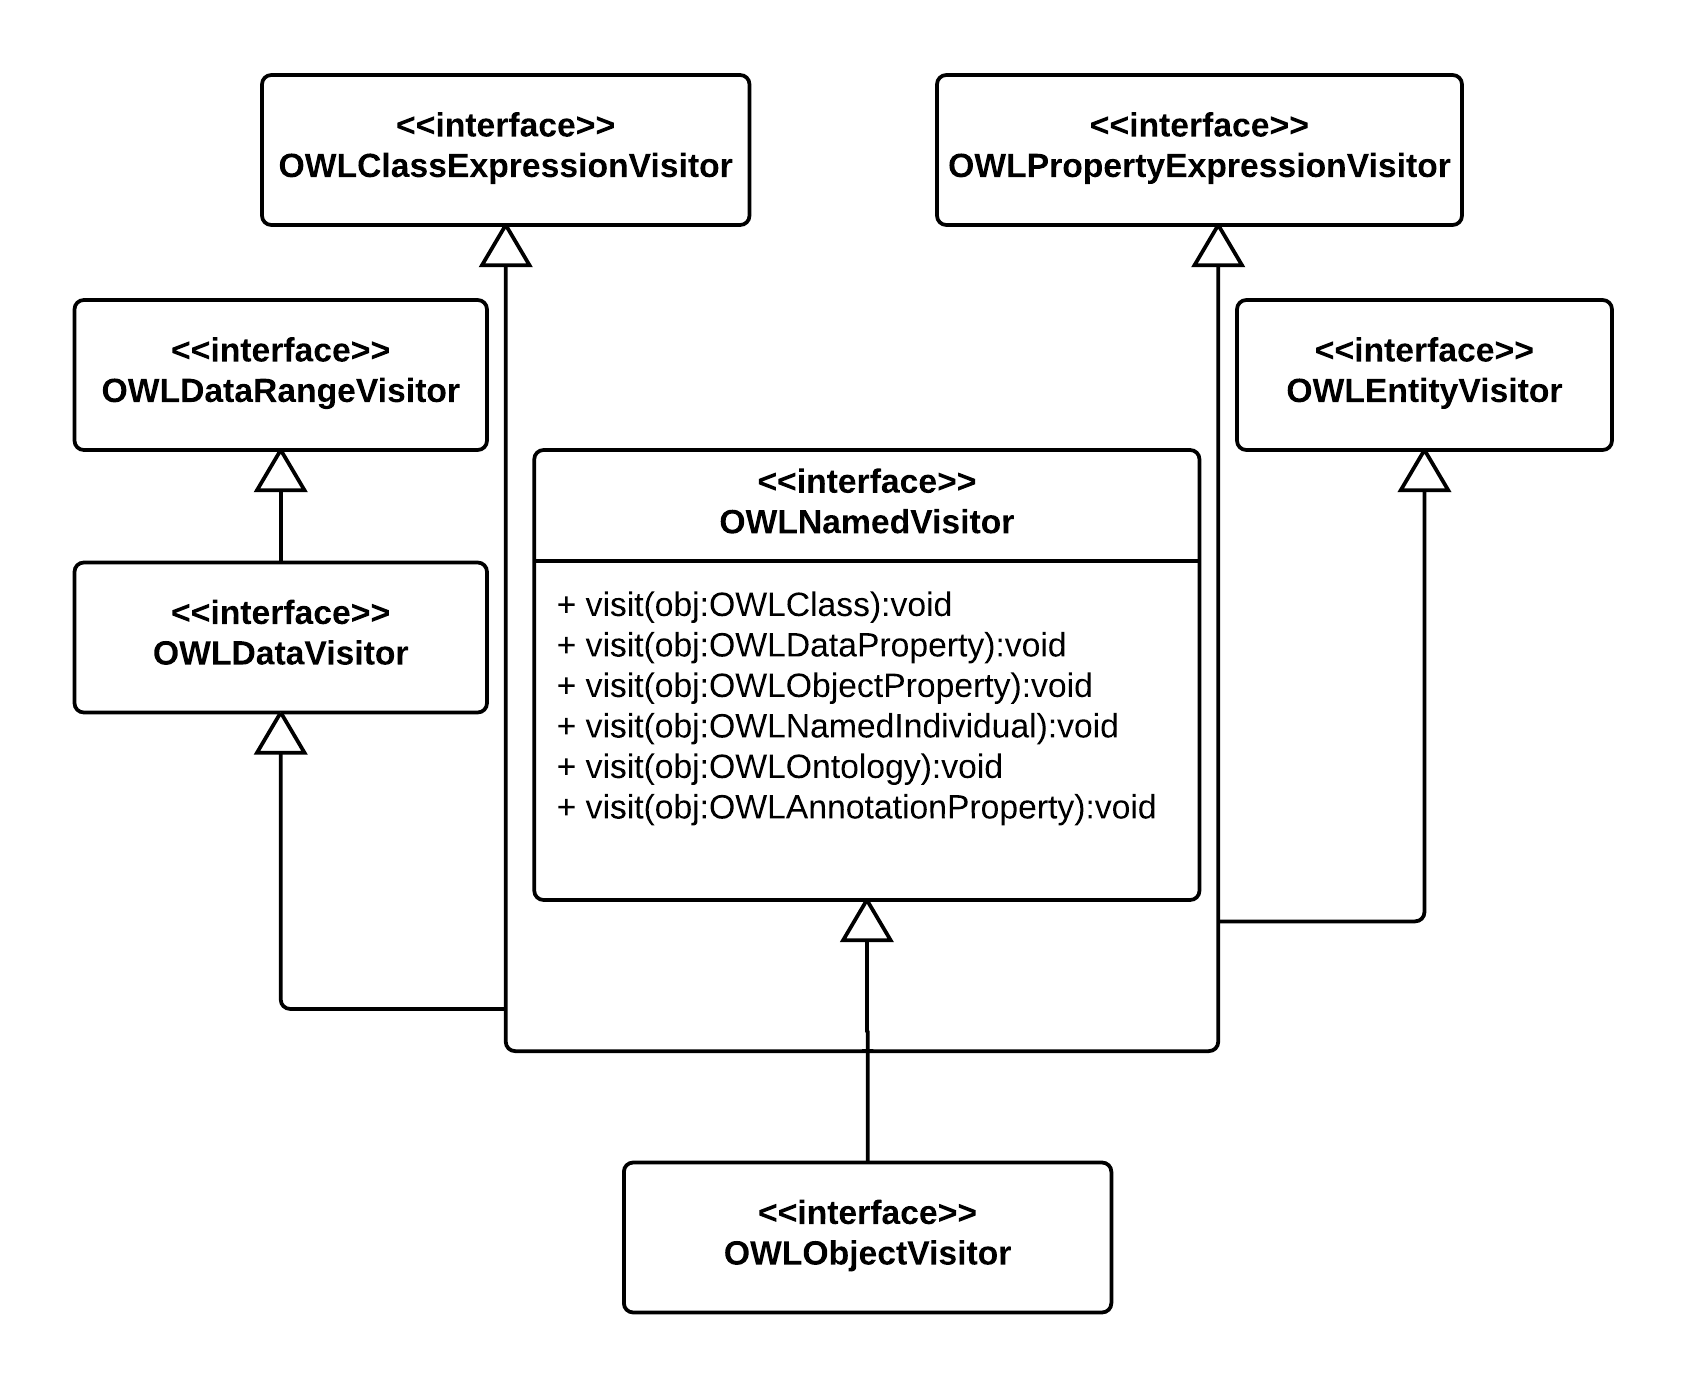
\includegraphics[width=145mm]{Figures/uml_classdiagram_owlobjectvisitor_nobackground.png}
	\caption{OWLObjectVisitor trong OWL-API \label{overflow}}
\end{figure}
Nhờ tận dụng tính đa hình trong lập trình hướng đối tượng nên các loại đối tượng thừa kế/mở rộng từ OWLObject đều có khả năng chấp nhận truy vấn lên chính nó (visitor.visit(this)) từ \textit{OWLObjectVisitor} (Hình 3.11).
\begin{figure}[h!]
	\centering
	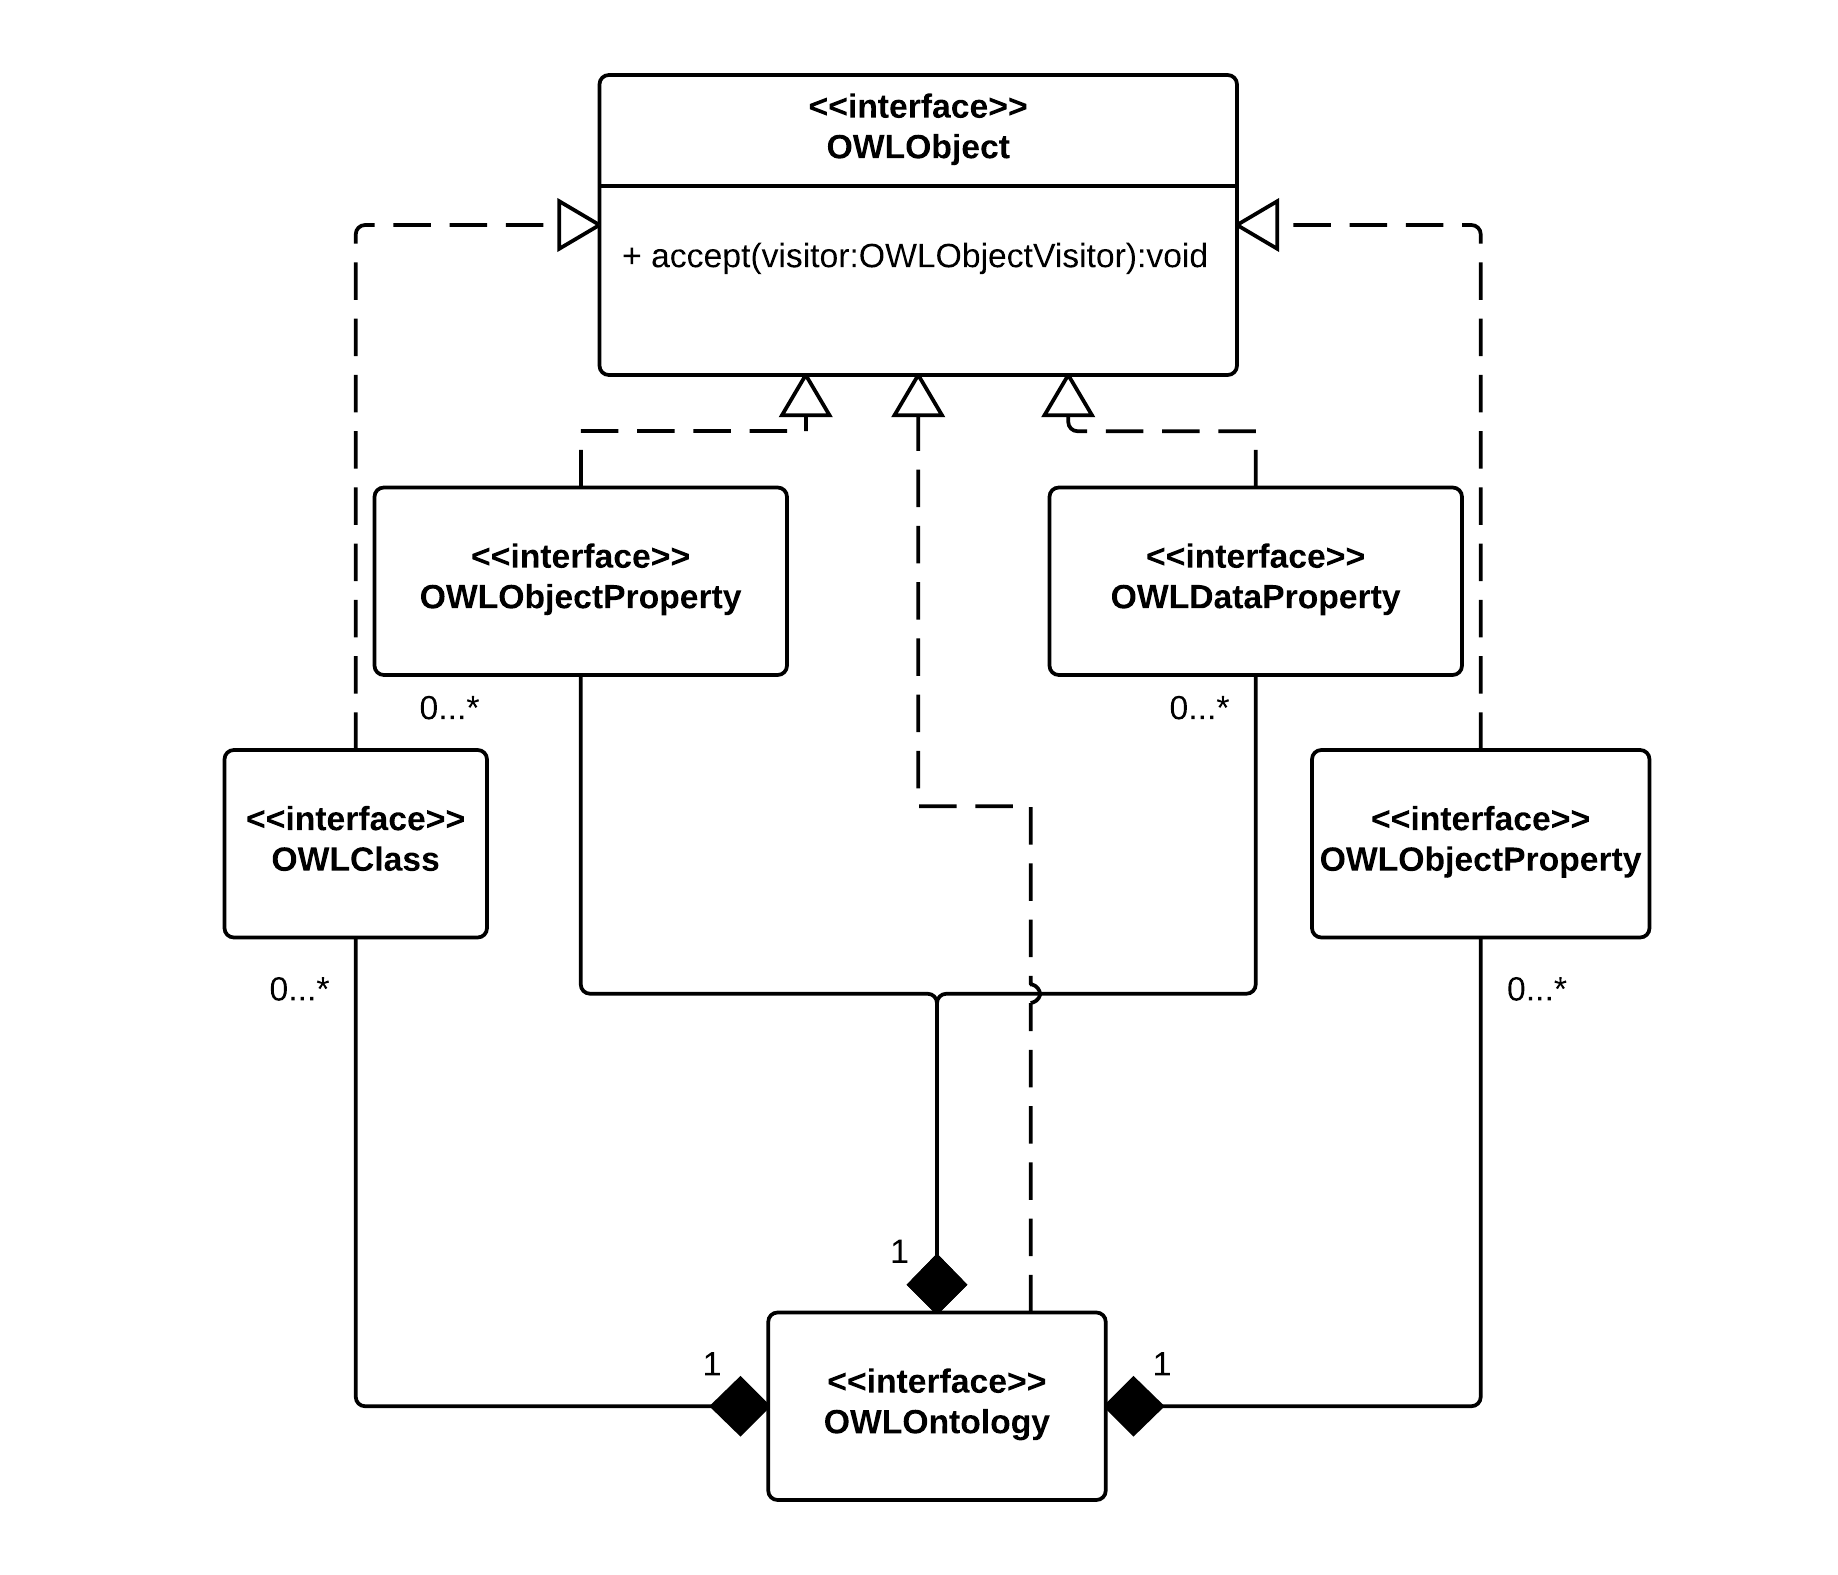
\includegraphics[width=145mm]{Figures/uml_classdiagram_owlobject_forvisitor_nobackground.png}
	\caption{OWLObject và OWLObjectVisitor trong OWL-API \label{overflow}}
\end{figure}
Để sử dụng các visitor, chúng em chỉ cần tạo các class áp dụng các interface tương ứng nhằm truy vấn dạng thành phần cụ thế như ví dụ OWLClassExpressionVisitor ở trên. Tuy nhiên, mỗi lần sử dụng là mỗi lần phải viết lại nội dung các phương thức trong Interface Visitor, để hạn chế sự lặp lại này OWL-API cũng cung cấp sẵn hoặc chúng ta cũng có thể tạo các class VisitorAdapter với nội dung mỗi phương thức được cài đặt tính năng mặc định. Ví dụ:
\begin{verbatim}
ClassExpressionVisitorAdapter implements OWLClassExpressionVistor {
  private void doNothing(OWLClassExpression ce) {};
  public void visit(OWLClass cls) {doNothing(cls);}
  public void visit(OWLObjectUnionOf union) {doNothing(cls);} ... }
\end{verbatim}
Mỗi khi muốn thay đổi nội dung phương thức nào chỉ cần \textit{Override} lại phương thức đó trong VisitorAdapter là được.
\section{Các tổ chức dữ liệu (data model) cho hệ thống}
Trong Vaadin Framework, dữ liệu trong lúc một ứng dụng đang ở trong tiến trình hoạt động được tổ chức thành các mô hình gọi là Data Model, với 3 cấp khác nhau gồm:Property, Item và Container. Có thể xem các \textit{Data Model} này như một đối tượng bao bọc (encapsulation) lại dữ liệu kiểu dữ liệu mà chúng ta muốn định nghĩa. Nếu câu hỏi là tại sao phải tốn công đưa các dữ liệu vào trong các đối tượng chứa như vậy, thì câu trả lời là vì Vaadin Framework cung cấp một cơ chế mà khi chúng ta tương tác với dữ liệu trong các \textit{Data Model} này thì đồng thời những thành phần giao diện (UI Components) cũng sẽ cập nhật các thay đổi đó. Lý do là vì hầu hết các thành phần giao diện đều được thiết kế độc lập với dữ liệu, dữ liệu được liên kết với các giao diện thông qua các \textit{Data Model} này. Sau đây chúng em xin trình bày cách tổ chức các đối tượng từ OWL-API vào trong các \textit{Data Model} là Property và Container (Item không được sử dụng vì không phù hợp với cấu trúc dữ liệu mà chúng em muốn tổ chức).

\subsection{Tổ chức các đối tượng OWL-API vào trong Property của Vaadin}
\begin{figure}[h!]
 	\centering
 	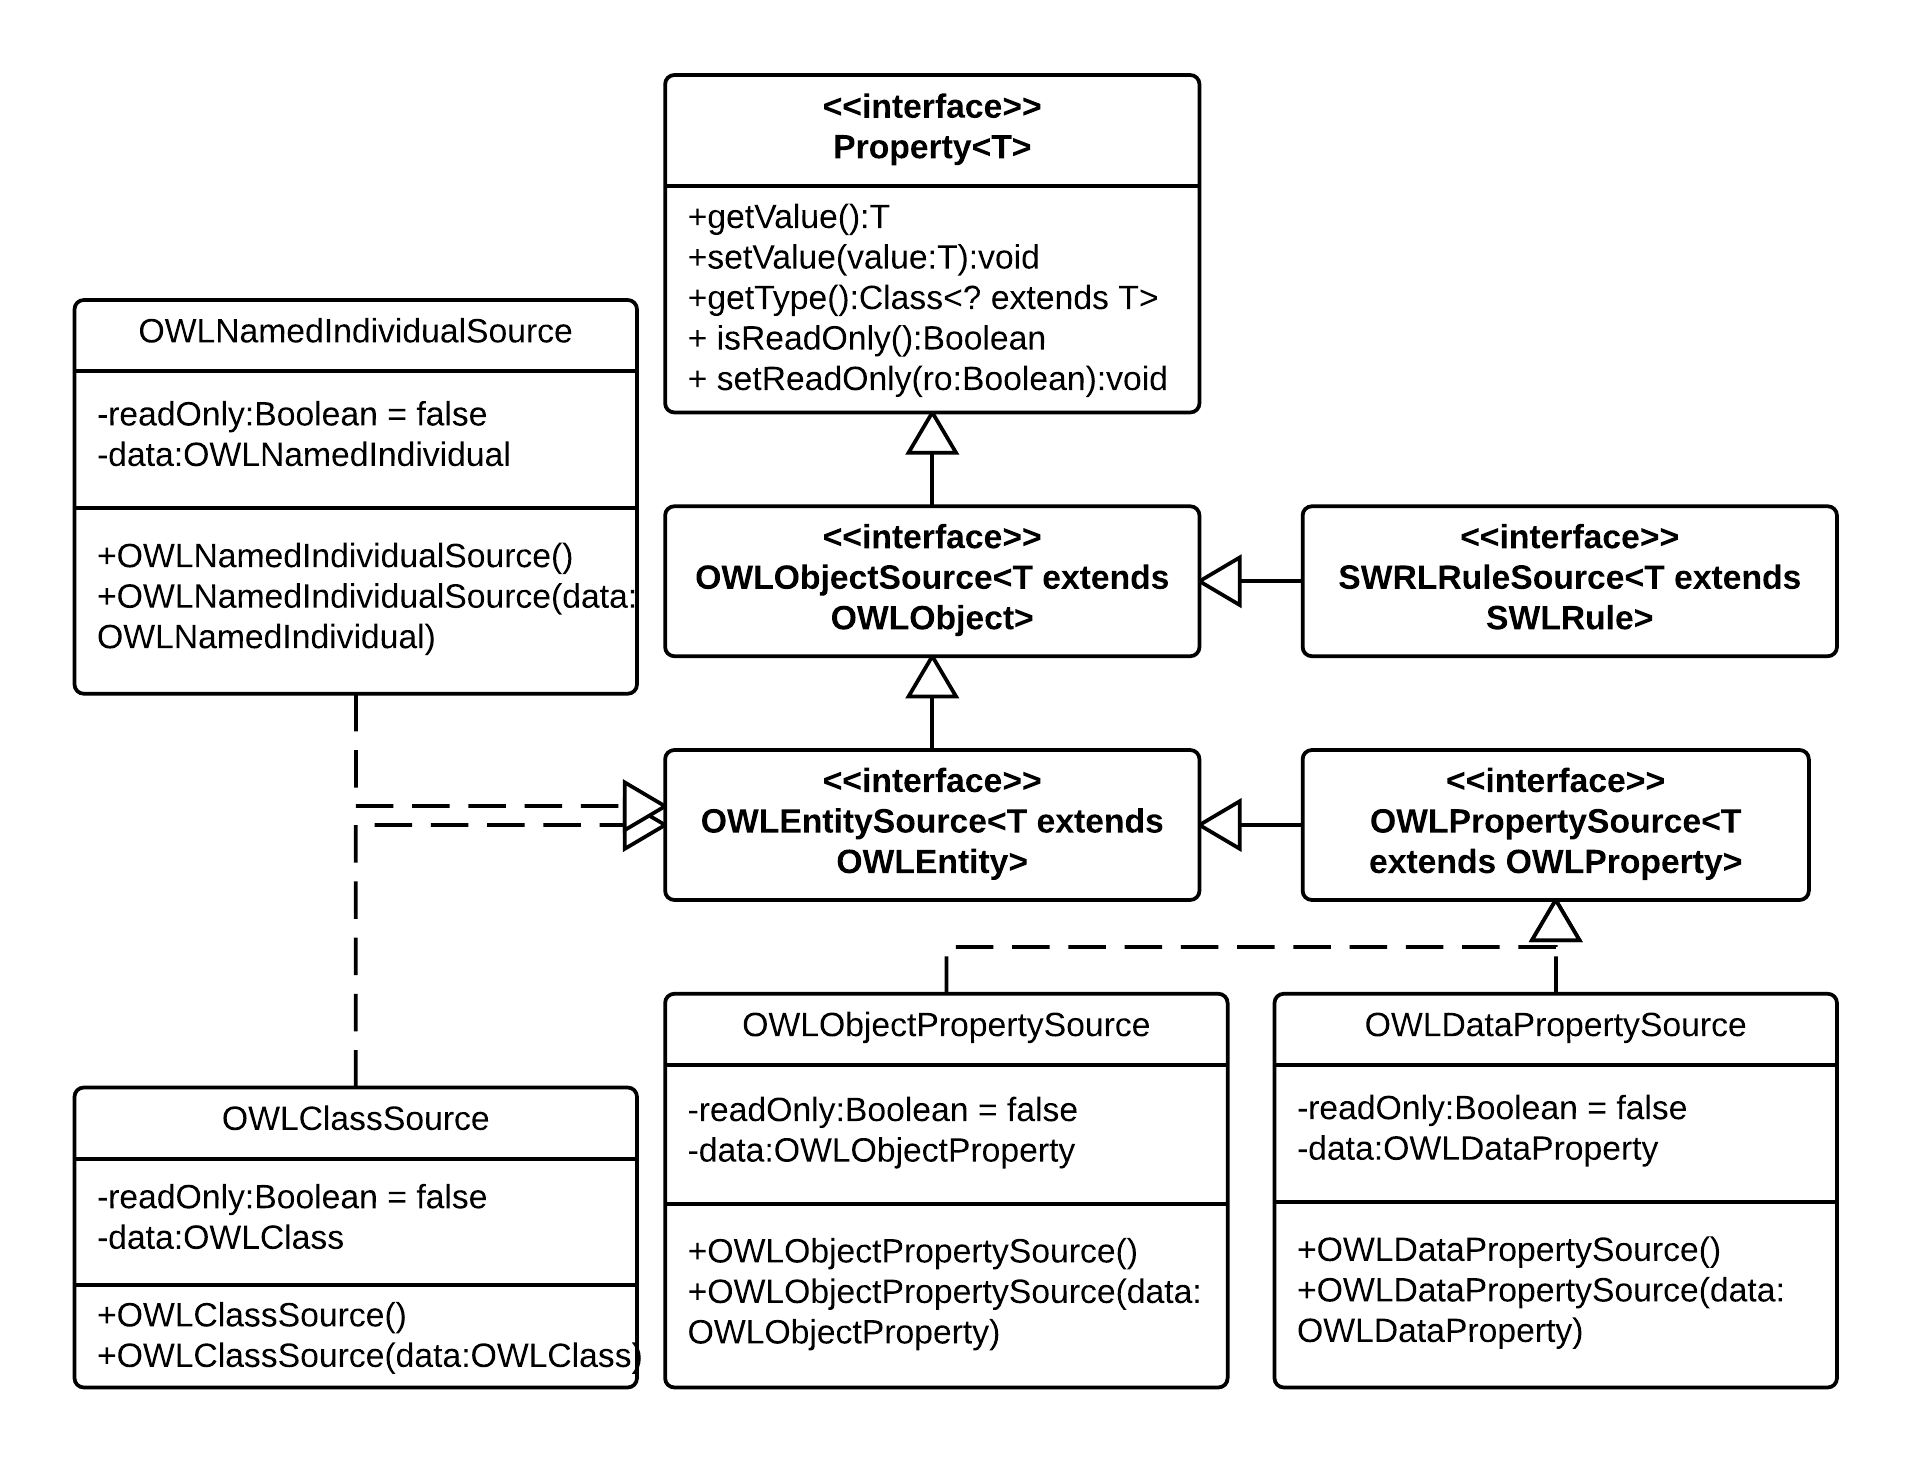
\includegraphics[width=150mm]{Figures/uml_owleditor_owlobjectsource.png}
 	\caption{Tổ chức dữ liệu dưới dạng Property \label{overflow}}
\end{figure}
\textbf{Property} là \textit{Data Model} đơn giản nhất, được Vaadin cung cấp dưới dạng Interface \textit{Property<T>} với $T$ kiểu dữ liệu được chúng ta định nghĩa, các thành phần giao diện như \textit{TextField}, \textit{Label}, \textit{TextArea} sử dụng \textit{Property} để liên kết dữ liệu với các đối tượng dữ liệu được định nghĩa qua $T$. Công việc phải làm là định nghĩa các \textit{Property} chứa các đối tượng OWL-API này. Do tính chất của OWL 2, ta có thế nói OWLClass (lớp) là một OWLEntity (thực thể), OWLEntity là một OWLObject (thành phần của OWL 2). Theo đó mà chúng em cũng sẽ tạo ra các Property tương ứng OWLObjectSource > OWLEntitySource > OWLClassSource. Việc tận dụng tính đa hình của đối tượng rất có ích khi xây dựng các UI Component chung cho các loại đối tượng giống nhau như OWLClass, OWLObjectProprerty, OWLDataProperty (cả đều mở rộng từ OWLEntity). 
\subsection{Tổ chức các thực thể OWLClass, OWLObjectProperty và OWLDataProperty thành các Container}
\begin{figure}[h!]
	\centering
	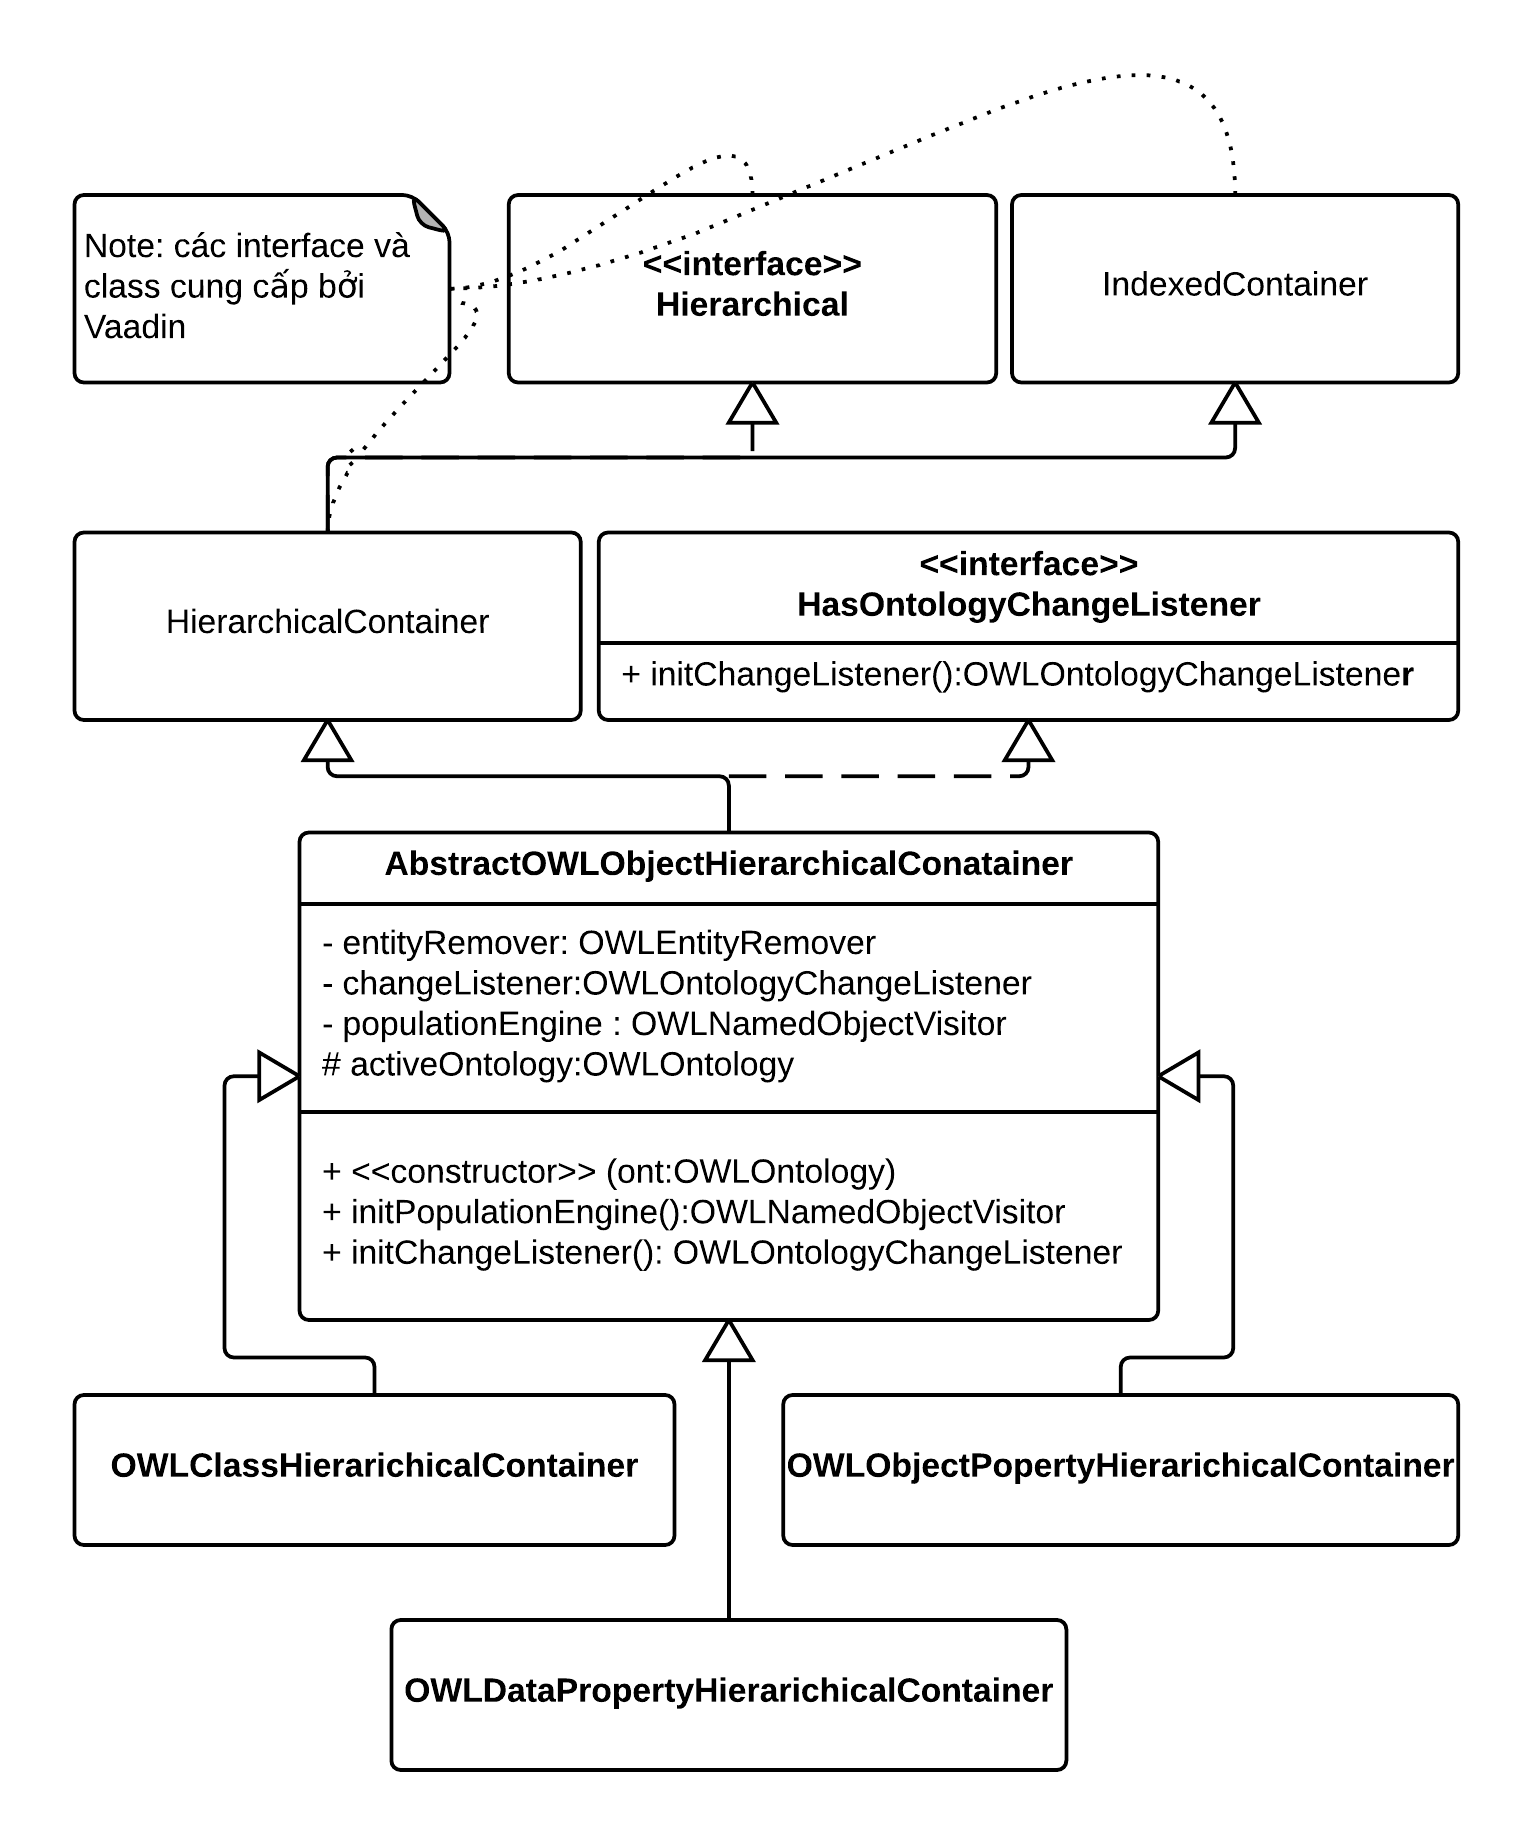
\includegraphics[width=150mm]{Figures/uml_owleditor_abstractcontainer_nobackground.png}
	\caption{Tổ chức các lớp, thuộc tính thành HierarchicalContainer \label{overflow}}
\end{figure}
\textbf{Container} là cấu trúc \textit{Data Model} phức tạp và cao nhất, chúng được chia thành các loại khác nhau tương ứng với tính chất của cấu trúc dữ liệu như \textit{HierarchicalContainer} dùng cho các cấu trúc dữ liệu phân cấp được hỗ trợ trong các thành phần giao diện (UI Component) như \textit{Table}, \textit{Tree}, \textit{ComboBox} và \textit{ListSelect}, đơn giản hơn có \textit{IndexedContainer} dùng cho cấu trúc dữ liệu dạng danh sách được hỗ trợ bởi \textit{ComboBox} và \textit{ListSelect} và \textit{JPAContainer} dùng cho các dữ liệu dạng SQL Table - hỗ trợ bở \textit{Table}, \textit{TreeTable}. Trong ứng dụng, chúng em chỉ sử dụng \textit{HierarchicalContainer} để tổ chức các lớp, thuộc tính đối tượng hay dữ liệu vì chúng cũng có tính chất phân cấp (SubClassOf, SubPropertyOf). Ở đây chúng em cũng xây dựng một AbstractClass rồi mở rộng ra với từng loại OWLEntity tương ứng là OWLClass, OWLObjectProperty và OWLDataProperty (Hình 3.13).

\section{Thiết kế cách xử lý sự kiện}
\subsection{Sử dụng Guava EventBus}
Do hệ thống gồm nhiều tab và các cửa sổ nhỏ (mô tả trong mục phác thảo giao diện), nên chúng em sẽ không áp dụng cách xử lý sự kiện truyền thống trong Java cho toàn hệ thống. Thay vào đó chúng em sử dụng một giải pháp thay thế là thư viện Guava EventBus - một nhánh nhỏ của thư viện Guava phát triển bởi Google \cite{guava}. Với Guava EventBus, mọi thành phần giao diện sẽ đăng ký các phương thức Subscriber - mỗi subscriber sẽ xử lý cho một loại sự kiện cụ thể -  với EventBus trong lúc khởi tạo hoặc hậu khởi tạo, sau đó EventBus lắng nghe mọi sự kiện được công bố lên eventBus bằng phương thức \textit{post}, cuối cùng EventBus bắt sự kiện và truyền sự kiện này đến đúng cho Subscriber nào đã đăng ký xử lý loại sự kiện này lúc đầu (Hình 3.14).
\begin{figure}[h!]
	\centering
	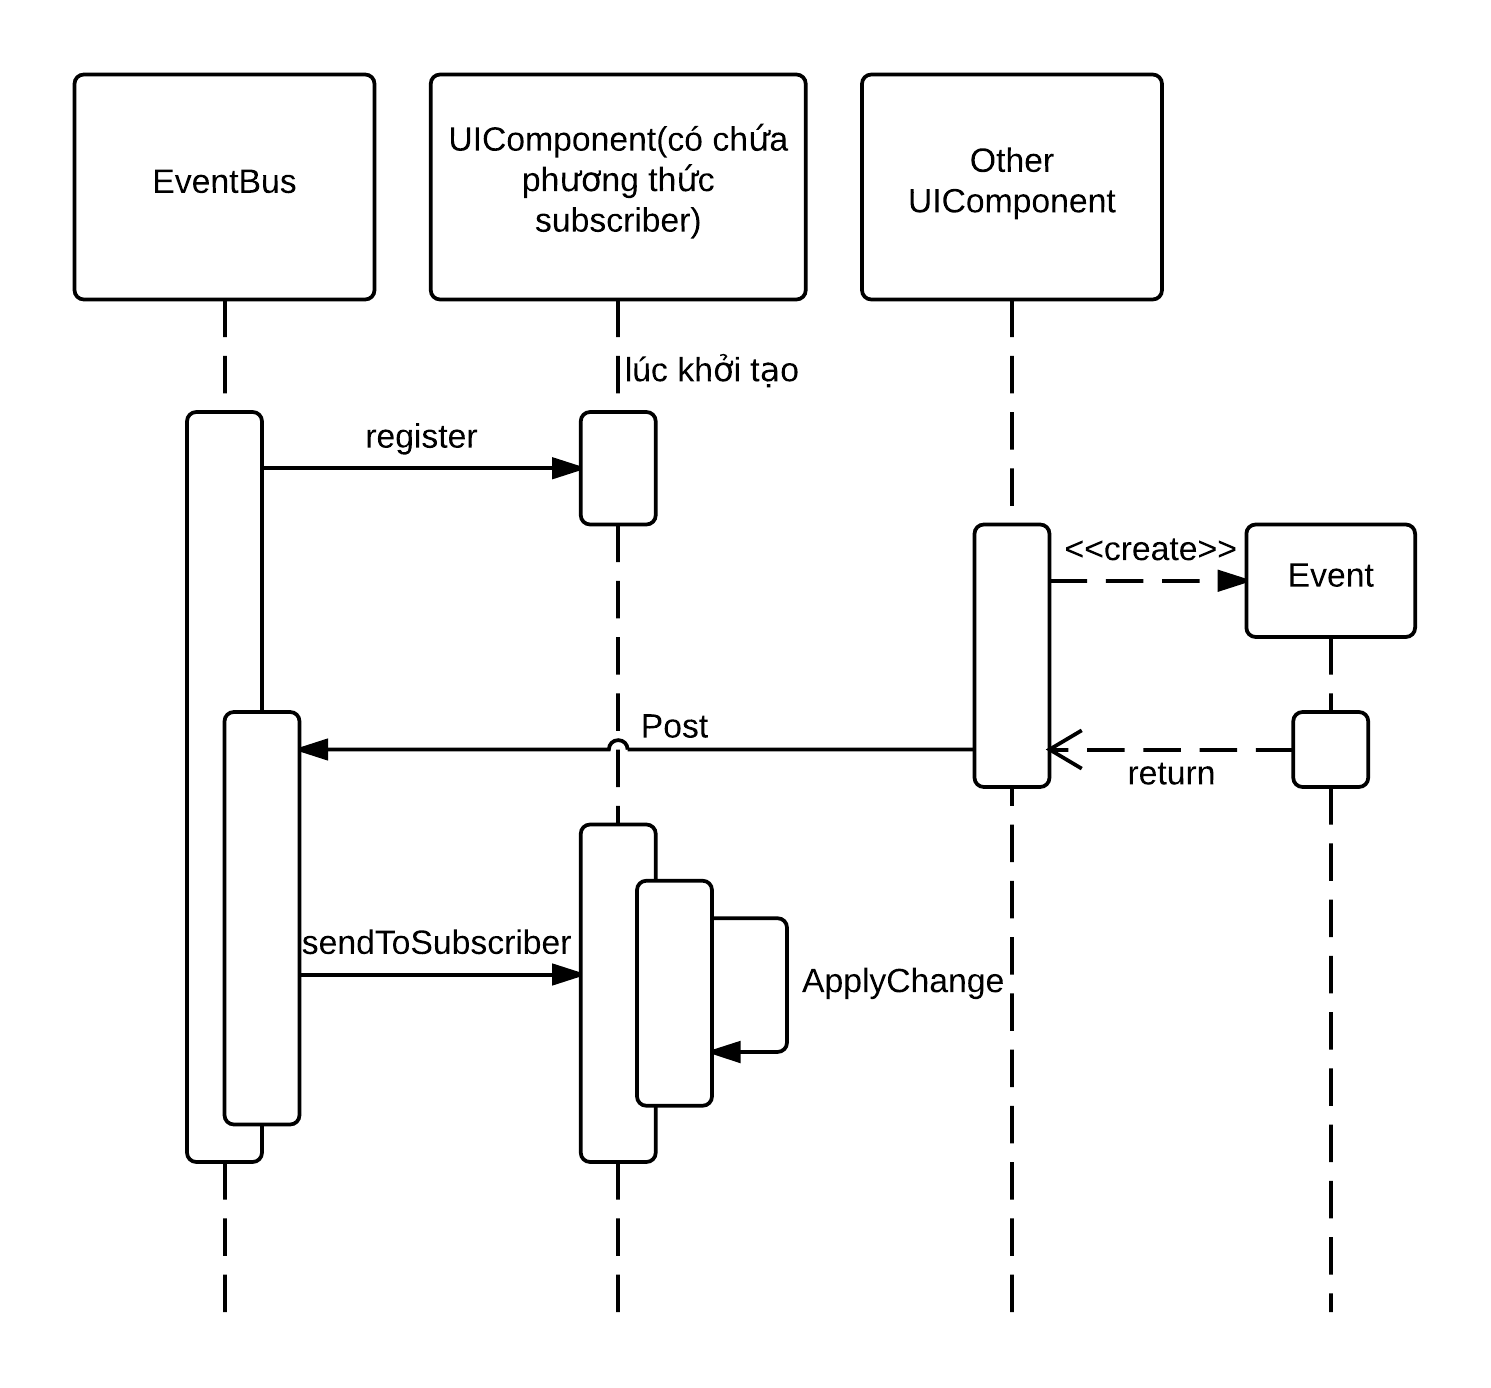
\includegraphics[height=115mm]{Figures/uml_eventbus_sequence.png}
	\caption{EventBus Sequence Diagram \label{overflow}}
\end{figure}
\\
UIComponent có thể được khai báo subscriber bằng Annotation @Subscriber cung cấp bởi thư viện Guava như sau:
\begin{verbatim}
public class SubscriberComponent {
  public SubscriberComponent { EventBus.register(this); }
  @Subscriber public void eventHandler(SpecificEventType event) { 
  	// các thay đổi được áp dụng ở đây  }
}
\end{verbatim}
EventBus có thể được sử dụng qua một lớp static với các phương thức register, post, unregister. Phương thức được chọn làm subscriber phải đáp ứng các yêu cầu sau đây:
\begin{itemize}
\item Khai báo public
\item Có duy nhất một tham số là sự kiện (event).
\item Không có kiểu trả về (return void).
\end{itemize}
\subsection{Các loại sự kiện trong hệ thống}
Do EventBus sẽ dựa vào loại Event để truyền đến đúng Subscriber cụ thể. Vì thế các loại sự kiện trong hệ thống sẽ được chúng em phân thành 3 loại dạng là thêm (add/create), xóa(remove), sửa (edit/modify) và phân thành 2 loại lớn là các sự kiện liên quan tới các thực thể và các sự kiện liên quan đến các phát biểu.
\begin{figure}[h!]
	\centering
	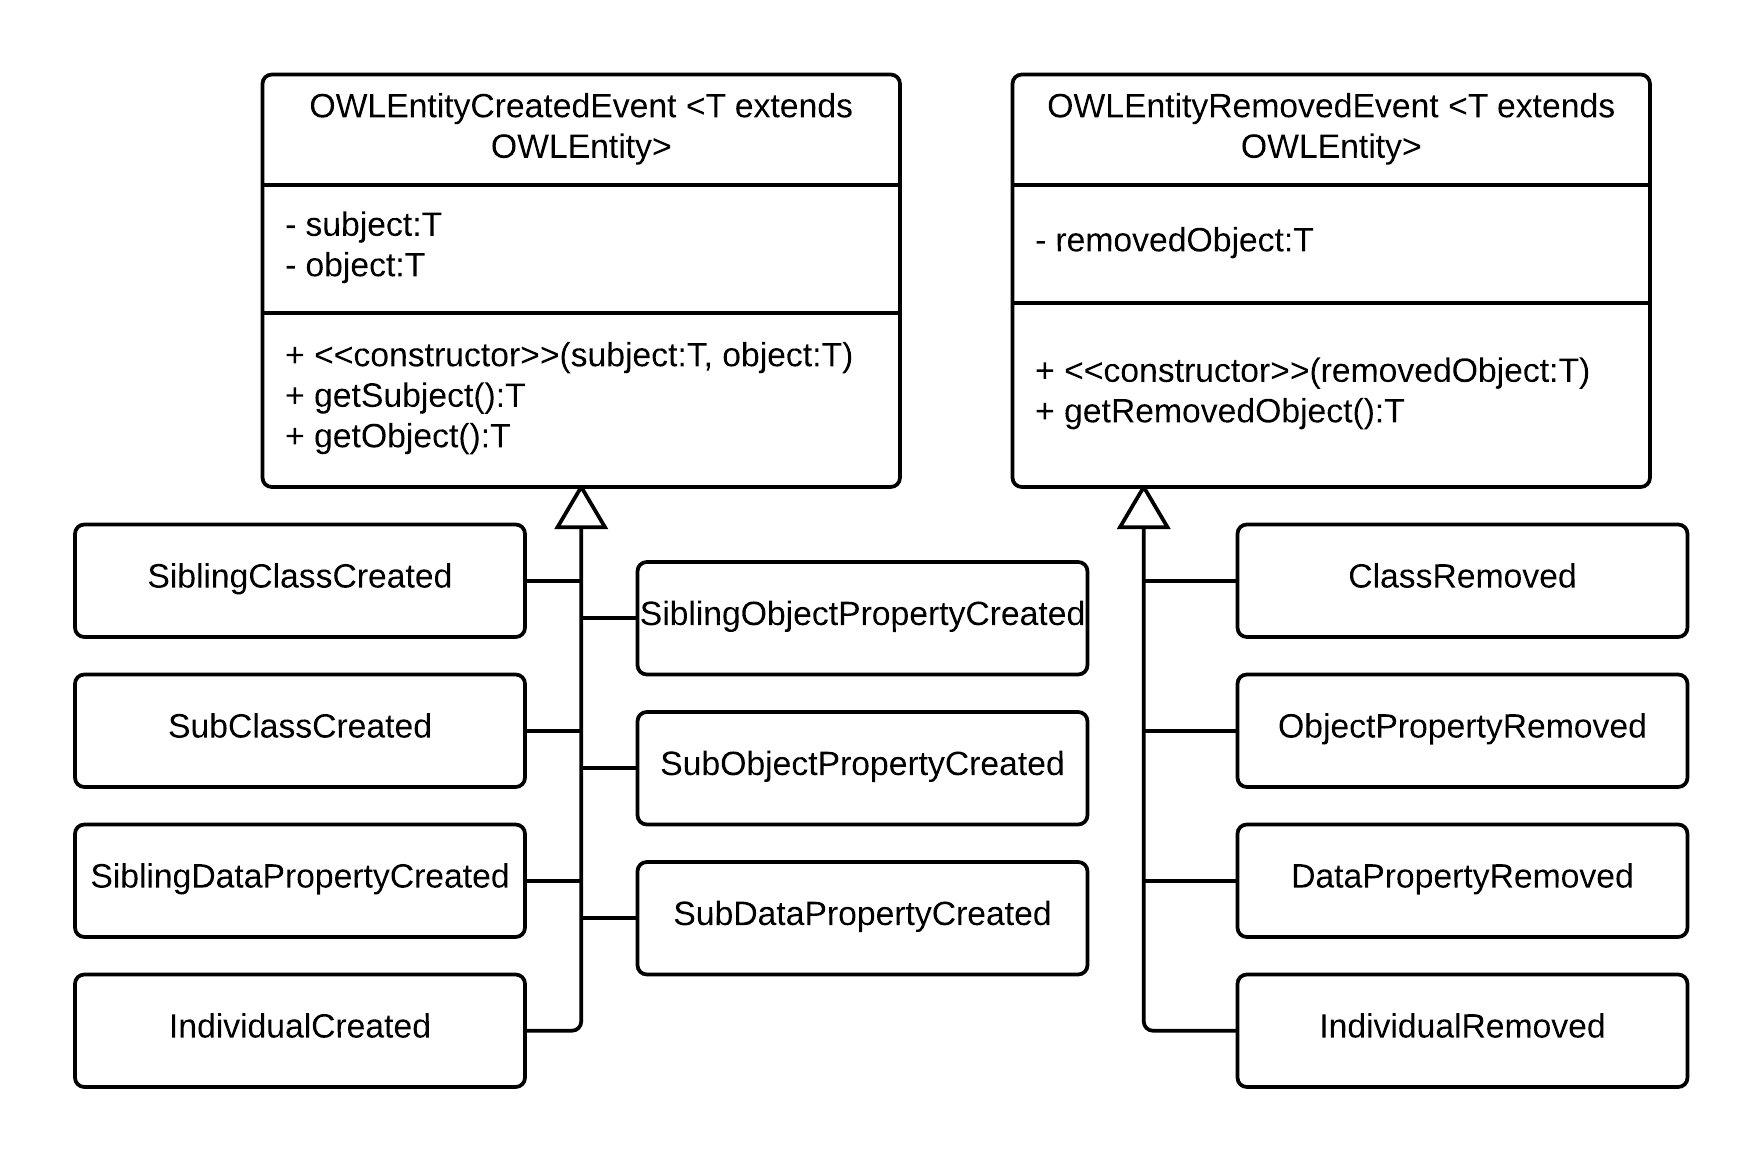
\includegraphics[width=150mm]{Figures/uml_entity_event.png}
	\caption{Các sự kiện của các cá thể\label{overflow}}
\end{figure}
\begin{figure}[h!]
	\centering
	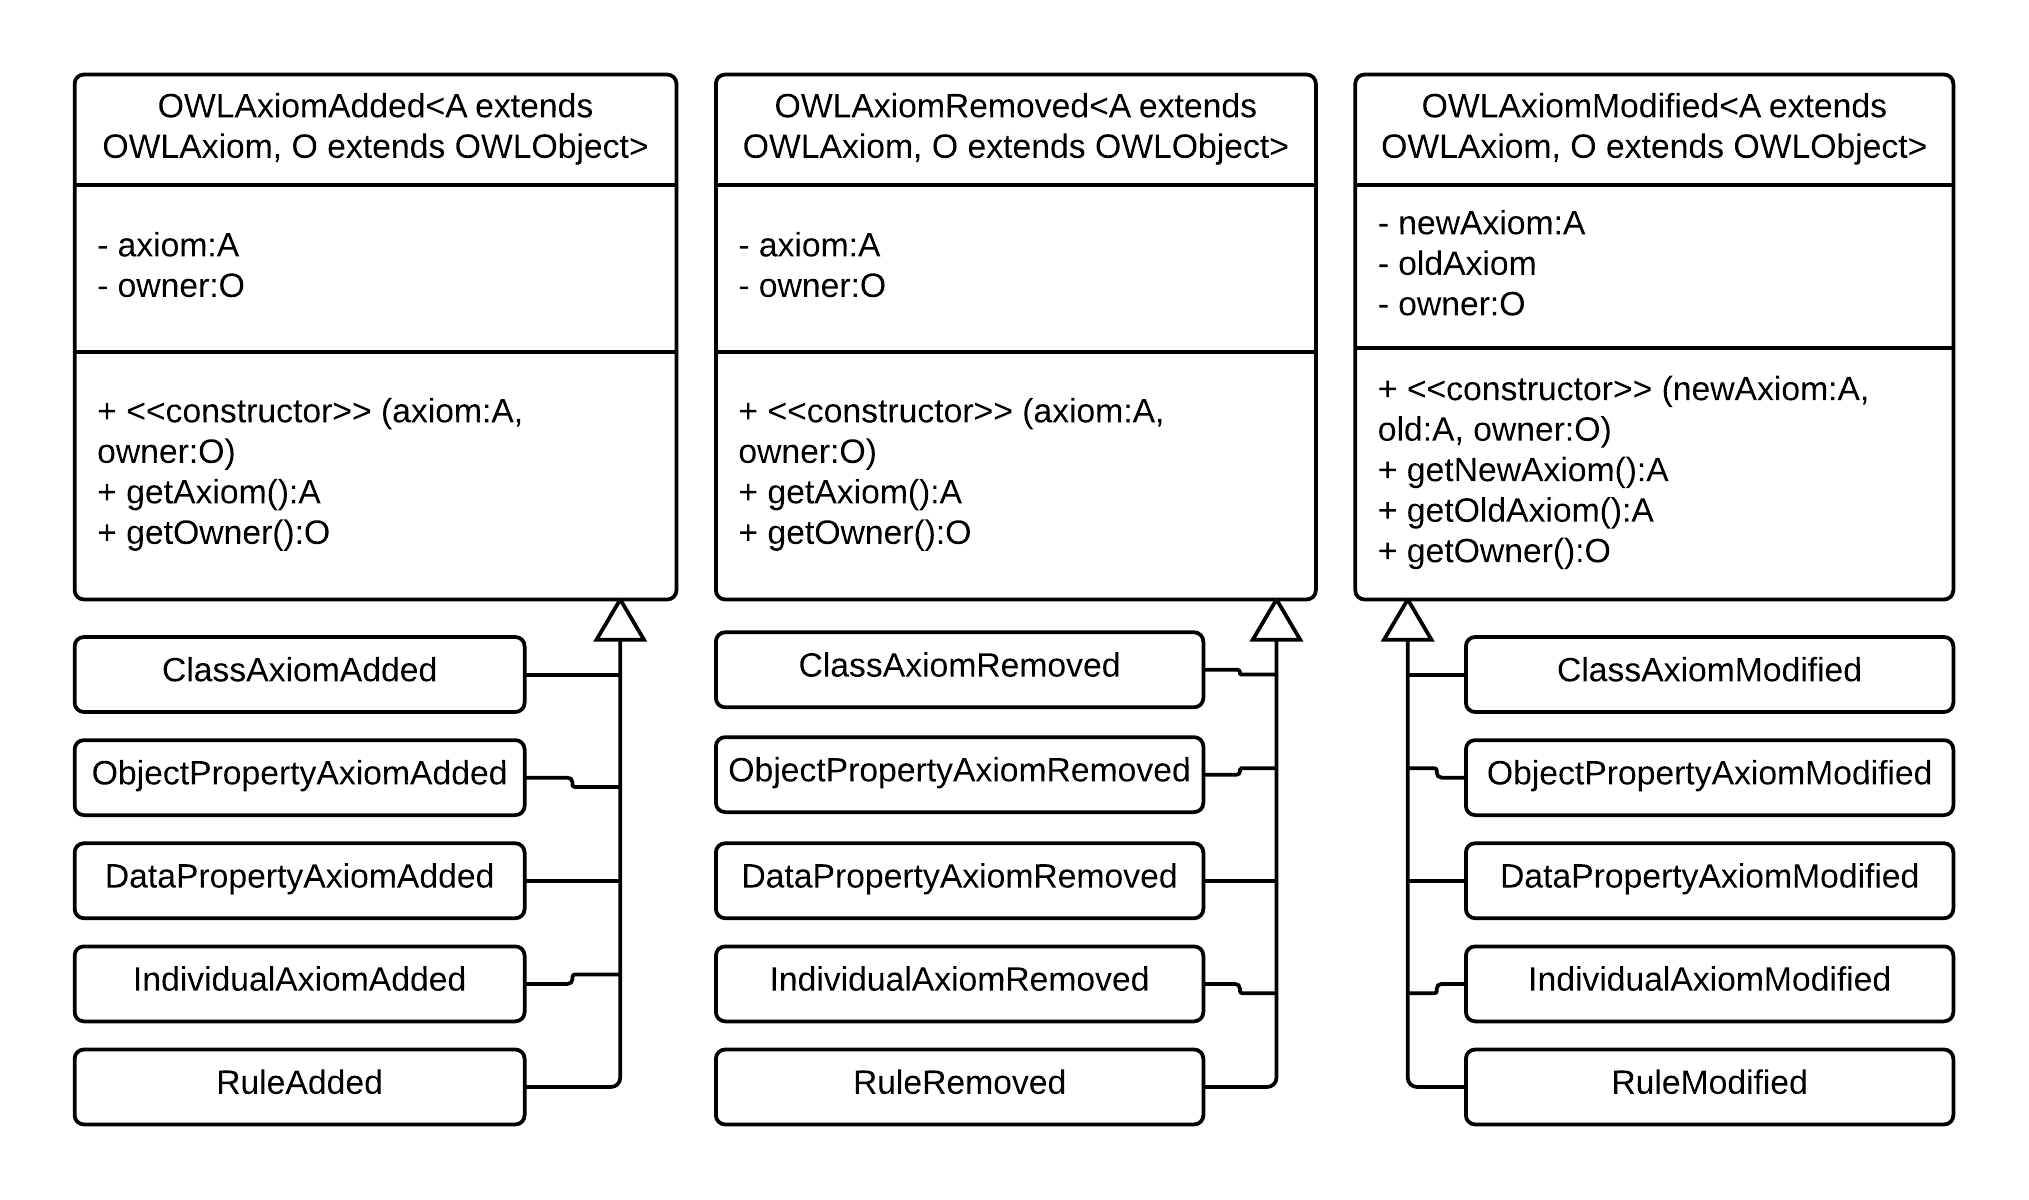
\includegraphics[height=97mm]{Figures/uml_axiom_event.png}
	\caption{Sự kiện cho các loại phát biểu \label{overflow}}
\end{figure}
Tên của các sự kiện cho cá thể gồm phần đầu là tên loại thực thể (Class, ObjectProperty, ...) và phần sau là động từ nói lên đó là sự kiện thêm, xóa hay sửa (Hình 3.15). Đối với sự kiện dành cho các phát biểu, tên của chúng gồm phần đầu nói lên loại phát biểu mà sự kiện đó đang xử lý và phần sau là động từ nói lên hành động thêm, xóa hay sửa (Hình 3.16).
\\
\section{OWLEditorKit}
\begin{description}
	\item[Interface:] \verb|vn.edu.uit.owleditor.OWLEditorKit|
	\item[Class implementation:] \verb|vn.edu.uit.owleditor.OWLEditorKitImpl|
\end{description}
Đây là thành quan trọng nhất của toàn bộ hệ thống được thiết kế để đảm nhiệm việc khai thác các API từ OWL-API, nạp/tạo Ontology từ IRI, suy luận, giải thích các phát biểu, parse các chuỗi viết theo cú pháp \textit{Manchester} thành các mô tả lớp và dữ liệu. Thực ra, các chứng năng vừa kể trên hầu hết đều được thực thi nhờ các API của OWL-API, \textit{OWLEditorKit} đóng gói tất cả lại thành một đối tượng để dễ dàng sử dụng trong các UI Component hơn, cũng như tránh việc phải khởi tạo nhiều lần các API. 
\subsection{Các chức năng của OWLEditorKit}

\subsubsection{Nạp Ontology}
Tương ứng với hàm \textit{loadOntologyFromOntologyDocument}, load các tài liệu OWL2 từ tham số là đối tượng \textit{IRI} của OWL-API, ontology khi load xong sẽ được gán cho đối tượng Active Ontology (sẽ được đề cập ngay sau).
\begin{verbatim}
OWLEditor kit = new OWLEditorKitImpl();
kit.loadOntologyFromOntologyDocument(IRI.create("some url"));
\end{verbatim}
\subsubsection{Giải thích các phát biểu trong OWL2 Ontology}
Việc này được thực hiện thông qua phương thức \textit{explain(OWLAxiom axiom)} của OWLEditorKit. Kết quả trả về là một đối tượng \textit{ExplanationTree}trong đó gồm các OWLAxiom (là các phát biểu giải thích). Cách sử dụng chi tiết hơn trong chương sau.

\subsubsection{Xóa các thực thể trong OWL2 Ontology}
Xóa các phát biểu trong OWL 2 Ontology không phải là một tác vụ dễ dàng vì một phát biểu có thể được sử dụng để xây dựng nên phát biểu khác. Ví dụ:
\begin{verbatim}
Declaration( Class( A ))
SubClassOf(A B)
EquivalentClasses(A C D)
\end{verbatim}
Giả sử chúng ta muốn xóa phát biểu \textit{Declaration( Class( A ))} thì \textbf{bắt buộc} chúng ta phải xóa luôn những phát biểu có liên quan đến A là \textit{SubClassOf và EquivalentClasses} bởi vì nếu không có phát biểu khẳng định sự tồn tại của A thì những phát biểu còn lại sẽ trở nên vô nghĩa. Tuy nhiên để thực hiện tác vụ này OWL-API cung đối tượng là \textit{OWLEntityRemover} với tính năng duyệt qua mọi phát biểu có liên quan đến thực thể cần xóa (thực ra OWLEntityRemover này cũng là một OWLObjectVisitor), xóa tất cả các phát biểu đó trước khi xóa thực thể. OWLEntityRemover được sử dụng thông phương thức \textit{getEntityRemover()} của OWLEditorKit. 
\begin{verbatim}
OWLClass person = ... ;
person.accept(editorKit.getEntityRemover()); // Xóa lớp person 
editorKit.getEntityRemover().reset(); // Cập nhật lại thông tin
\end{verbatim}

\subsubsection{Tạo ra các thành phần OWL 2 bằng OWLDataFactory}
Một chức năng thực sự hữu ích cung cấp bởi OWL-API, với số lượng đối tượng (thực thể, mô tả lớp, thuộc tính, phát biểu, ...) rất lớn đã đề cập ở chương 2, rất khó để chúng ta có thể nhớ và sử dụng chúng dễ dàng. \textit{OWLDataFactory} hoạt động như một nhà máy tạo ra hầu hết các loại phát biểu, thực thể, kiểu dữ liệu trong OWL 2 Ontology một cách tiện lợi. Ví dụ như:
\begin{verbatim}
// Declaration( NamedIndividual(a:Peter) )
OWLNamedIndividual Peter = factory.getOWLNameIndividual("a:Peter");
// Declaration( DataProperty(a:HasAge) )
OWLDataProperty hasAge = factory.getOWLDataProperty("a:HasAge");
// ClassAssertion( a:Person a:Peter )
OWLLiteral age = factory.getOWLLiteral(22);
\end{verbatim}
Trong hệ thống, OWLDataFactory được sử dụng qua phương thức \textit{getOWLDataFactory()} của OWLEditorKit.

\subsubsection{Tạo ra các Data Model và Event bằng EditorDataFactory}
{\let\thefootnote\relax\footnotetext{
		*: \textit{http://en.wikipedia.org/wiki/Factory\_method\_pattern}}
}
Học tập mô hình \textit{Factory Pattern} \textsuperscript{*} từ \textit{OWLDataFactory}, chúng em cũng tự xây dựng một factory để tạo ra các đối tượng dữ liệu và các event trong ứng dụng. Ví dụ:
\begin{verbatim}
OWLClass person, man; OWLEditorKit kit = ...; 
OWLEditorFactory fc = new OWLEditorFactoryImpl(kit);
ClassAxiomAdded event = fc.getSubClassOfAddEvent(man, person);
OWLClassHierarchicalContainer con = 
               fc.getClassHierarchicalContainer(kit.getActiveOntology)
\end{verbatim}

\subsubsection{Parse chuỗi thành các mô tả lớp (OWLClassExpression)}
OWLEditorKit cũng được tích hợp một đối tượng \textit{ManchesterOWLSyntaxParser} trong OWL-API, nhiệm vụ là để parse các đoạn text từ người dùng theo cú pháp \textit{Manchester} thành các mô tả lớp (OWLClassExpression) hay các miền dữ liệu (OWLDataRange). Parser này được sử dụng thông qua getter \textit{getParser} hoặc parse trực tiếp qua hàm \textit{parseClassExpression(String stringToParse)} . Ví dụ:
\begin{verbatim}
OWLEditorKit eKit = new OWLEditorKitImpl(); // nạp ontology ...
OWLClassExpression ce2 = eKit.parseClassExpression("Has some Kid");
\end{verbatim}

\subsubsection{Suy luận các phát biểu}
PelletReasoner cũng được chứa trong OWLEditorKit, được sử dụng qua phương thức \textit{getReasoner()}. Cách sử dụng:
\begin{verbatim}
OWLNamedIndividual peter = ...; 
// Tìm xem Peter thuộc những lớp nào
editorKit.getReasoner().getTypes(peter,true).getFlattened();
OWLClass driver = ...;
// Tìm lớp con 
editorKit.getResoner().getSubClasses(driver,true).getFlattened();
\end{verbatim}
True nghĩa là chỉ tìm lớp gần nhất cho việc giải thích. Giả sử cá thể Peter thuộc các lớp driver mà Driver là lớp con của Person. Nếu để \textit{true} thì kết quả chỉ có Driver và ngược lại thì kết quả gồm Driver và Person. Tương tự cho SubClass, SubProperty, ... .
\subsubsection{Quản lý các Ontologies được nạp và áp dụng các thay đổi}
Việc nạp ontology, thực sự diễn ra bên trong lớp OWLEditorKitImpl và được thực hiện bởi \textit{OWLOntologyManager} - api của OWL-API.  Ontology nạp vào sẽ được quản lý theo OntologyIRI và VersionIRI (xem ở chương 2).
\begin{verbatim}
OWLEditorKitImpl implements OWLEditorKit { ...
  OWLOntologyManager manager = new OWLManager.getOWLOntologyManager();
  public void loadOntologyFromOntologyDocument(IRI iri) {
  	manager.loadOntologyFromOntologyDocument(iri);
  }
}
\end{verbatim}
Ngoài chức năng trên, OWLOntologyManager còn được sử dụng để áp dụng các thay đổi lên Ontology, các thao tác chỉnh sửa sẽ vô nghĩa nếu kết quả của chúng không được áp dụng lên Ontology. Chúng ta sử dụng OWLOntologyManager cho tác vụ này qua phương thức \textit{getModelManager()} như sau:
\begin{verbatim}
OWLEditorKit kit = ...; fc = kit.getOWLDataFactory();
OWLClass vehicle = fc.getOWLClass("a:Vehicle"); 
OWLAxiom clsAxiom = fc.getOWLClassDeclarationAxiom(vehicle);
kit.getModelManager()
   .applyChange(new AddAxiom(clsAxiom, kit.getActiveOntology());
\end{verbatim}
\subsubsection{Quản lý, thao tác với các SWRL Rule}
Trong cài đặt của OWLEditorKit, cũng bao gồm SWRLAPIOntology (từ SWRLAPI \cite{swrlapi}) dùng quản lý và thêm/xóa/sửa SWRL Rule. Đối tượng này được sử dụng qua phương thức \textit{getSWRLActiveOntology()} của OWLEditorKit. Lưu ý: SWRLAPIRule (từ thư viện SWRL-API) được mở rộng từ SWRLRule (từ thư viện OWL-API).
\begin{verbatim}
SWRLAPIOntology ruleOntology = editorKit.getSWRLActiveOntology();
Set<SWRLAPIRule> allRules = ruleOntology.getSWRLAPIRules();
\end{verbatim}
Tóm lại, mọi thao tác lên ontology từ bất kì thành phần giao diện nào đều phải thông qua sử dụng các phương thức mà OWLEditorKit cung cấp.

Tóm lại, mọi thao tác lên ontology đều từ bất kì thành phần giao diện nào đều phải các phương thức mà OWLEditorKit cung cấp.
\section{Xây dựng một ontology để trình bày quá trình phân loại}
\textbf{Giới thiệu} Transport.owl \cite{owleditorSrc} là một ontology do nhóm tự xây dựng nên, đối tượng chủ yếu là các phương tiện giao thông đường bộ, đường thuỷ, đường hàng không, bên cạnh đó là các bộ phận của phương tiện như động cơ, rô-tơ,... các đối tượng liên quan như hàng hoá, hành khách, bộ phận của phương tiện, ... .Ontology được thiết kế nhằm biểu diễn đặc tính phân loại của OWL 2 và SWRL, nên có một vài điểm không bám sát theo đúng với thực tế. Sau đây chúng em xin được miêu tả ontology này.
\subsection{Cấu trúc phân lớp của ontology}



%\chapter{Công nghệ sử dụng}
\paragraph{Giới thiệu} Trong chương này, chúng em xin giới thiệu qua các thư viện lập trình (API) và framework được sử dụng để xây dựng chương trình. Các thư viện sử dụng gồm có OWLAPI \cite{owlapi}, SWRLAPI \cite{swrlapi}, Pellet \cite{pellet} và thành phần giúp tạo nên giao diện người dùng của ứng dụng - Vaadin Framework. Đầu tiên xin được giới thư viện lập trình OWL-API.
\section{Thư viện lập trình OWLAPI}
Thư viện lập trình Ontology Web Language là một thư viện mã nguồn mở (phát hành dưới 2 giấy phép \textbf{LGPL} và \textbf{Apache}) \cite{owlapi} được viết bằng JAVA với mục đích hỗ trợ các lập trình viên phát triển các ứng dụng có liên quan đến OWL2 Ontology. Tính đến thời điểm hiện tại thư viện đã được phát triển đến phiên bản 4.0 - cũng là phiên bản được sử dụng trong ứng dụng của chúng em.
Thư viện có các thành phần chính như sau: 
\begin{itemize}
	\item API để tương tác với các thành phần của OWL 2 được đề cập trong chương 2.
	\item Renderer và Parser (dùng đọc và ghi OWL 2 Ontology) nhiều dạng cú pháp khác nhau đã đề cập ở chương 2 như \textit{RDF/XML}, \textit{OWL/XML}, \textit{OWL Functional Syntax}, \textit{Manchester OWL Syntax} và \textit{Turtle}.
	\item Reasoner Interfaces cho các reasoners khác nhau hỗ trợ cho việc suy luận.
\end{itemize}
Danh sách các Ontology Reasoner được hỗ trợ trong phiên bản 4.0: FaCT++, Hermit, Pellet \cite{pellet}, JFact.
Các đối thành phần (thực thể, mô tả lớp/thuộc tính,...) được giải thích trong lúc giới thiệu OWL 2 đều đươc OWL-API mô hình hóa thành các đối trượng trong Java, với tiếp đầu ngữ \textit{OWL} + tên thành phần. Ví dụ:
\begin{verbatim}
Class              -> OWLClass  #Lớp
ObjectProperty     -> OWLObjectProperty # thuộc tính đối tượng
OWLClassExpression -> OWLClassExpression # Mô tả lớp
\end{verbatim} 
Tương tự cho các thành phần khác. Để tương tác với một cấu trúc gồm nhiều thành phần phân cấp như các thành phần của OWL 2 ontology cần có cách thức chuyên dùng cho việc này là Visitor Pattern.
\subsection{Visitor Pattern}
\begin{figure}[h!]
	\centering
	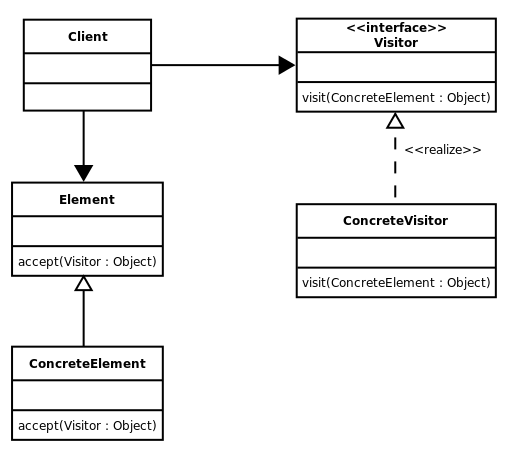
\includegraphics[width=110mm]{Figures/visitor_diagram.png}
	\caption{Visitor Diagram\label{overflow}}
\end{figure}
\paragraph{Khái quát} Trong lập trình hướng đối tượng và phát triển ứng dụng, Visitor Pattern hay Visitor Design Pattern là một cách để tách biệt một giải thuật ra khỏi cấu trúc của đối tượng mà nó đang xử lý. Nhờ sự tách biệt này, chúng ta có khả năng thêm một tính năng mới cho đối tượng mà không cần phải sửa đổi cấu trúc của đối tượng đó. Lấy ví dụ một visitor trong thư viện OWL-API là \textit{OWLClassExpressionVisitor}, chúng ta đã biết bên dưới có rất nhiều đối tượng thừa kế từ OWLClassExpression (mô tả lớp) như OWLObjectUnionOf, OWLObjectIntersectionOf, OWLClass, OWLObjectAllValueFrom, OWLObjectSomeValuesFrom,... Chúng ta xem qua các đoạn code sau :
\begin{verbatim}
// visitor interface
public interface OWLClassExpressionVisitor {
     public void visit(OWLClass cls);
     public void visit(OWLObjectUnionOf union);
     ...
}
// Lớp visitor
public class OWLClassExpressionVisitorImpl 
                 implements OWLClassExpressionVisitor {
    public void visit(OWLClass cls) {
        System.out.println("Lớp:" + cls.toString()); // (4)
    }
    public void visit(OWLObjectUnionOf union) {
        // Hàm getOperands trả về các mô tả lớp trong phát biểu unionOf
        for(OWLClassExpression ce: union.getOperands()) {
           ce.accept(this); // (2), (2')
        }
	}
	...
}
// Interface OWLClassExpression
public interface OWLClassExpression {
    public void accept(OWLClassExpressionVisitor visitor);
}
// Lớp OWLObjectUnionOf thừa kế từ OWLClassExpression
public class OWLObjectUnionOfImpl implements OWLClassExpression {
	public void accept(OWLClassExpressionVisitor visitor) {
    	visitor.visit(this); // (1)
    }
    ...
}
// Lớp OWLClass thừa kế từ OWLClassExpression 
public class OWLClass implements OWLClassExpression {
    public void accept(OWLClassExpressionVisitor visitor) {
        visitor.visit(this); // (3)
    }
    ...
}
// Hàm main 
public void main(String[] args) {
   OWLDataFactory factory = OWLManager.getOWLDataFactory();
   OWLClass car = factory.getOWLClass("a:Car");
   OWLClass bike = factory.getOWLClass("a:Bike");
   OWLObjectUnionOf union = factory.getOWLObjectUnionOf(car, bike);
   OWLClassExpressionVisitor visitor = new OWLClassExpressionVisitorImpl();
   union.accept(visitor);                                       
}
// Output của hàm main sẽ là 
Lớp: a:Car
Lớp: a:Bike
\end{verbatim}
Đối tượng \textit{OWLDataFactory} sẽ được trình bày ở mục sau, chúng ta có thể hiểu hàm \textit{main} như sau factory tạo ra 2 đối tượng OWLClass là car, bike tương đương với 2 lớp trong OWL2 a:Car, a:Bike, tiếp đó factory tạo ra một đối tượng union tương đương \textit{ObjectUnionOf( a:Car a:Bike )} trong OWL2. Cuối cùng ta sử dụng cho union.accept(visitor) thì thứ tự gọi hàm cho tới khi in ra từng dòng output là (1),(2),(3) và (4). 
\\
Đây chính là cách một \textit{visitor} hoạt động, thư viện OWL-API sử dụng lặp đi, lặp lại rất nhiều lần các interface visitor cho nhiều tác vụ khác nhau từ parser (dịch raw text thành cú pháp của OWL 2), renderer(dùng đọc các thành phần của ontology) như ví dụ trên qua các interface như OWLObjectVisitor, OWLDatatypeVisitor,... hoặc đọc và dịch SWRL Rule qua interface SWRLObjectVisitor. Chúng em cũng sử dụng \textit{Visitor Pattern} rất nhiều lần trong ứng dụng của mình để thực hiện nhiều tác vụ tương tự.
\subsection{Một số hàm hữu ích khi sử dụng OWL-API}
\subsubsection{EntitySearcher}
Static class \verb|EntitySearcher| cho phép truy vấn đến các cá thể trong OWL2 Ontology một cách nhanh nhất nếu chúng đã được khai báo. Ví dụ để tìm các mô tả lớp con của một lớp nào đó trong OWL 2 Ontology:
\begin{verbatim}
OWLOntology ont = modelManager.loadOntologyFromOntologyDocument(ontologyIRI);
OWLClass person = factory.getOWLClass("a:Person");
// Tìm các lớp con của person trong ontology "ont"
Collection<OWLCLassExpression> subClasses = 
			EntitySearcher.getSubClasses(person, ont);
			
\end{verbatim}
Lưu ý: Cần phân biệt các tính năng của \verb|EntitySearcher| với thành phần reasoner vì reasoner cũng có các hàm đảm nhiệm tính năng tương tự. EntitySearher chỉ tìm những phát biểu \textbf{đã} khai báo trong ontology, còn Reasoner tìm những phát biểu \textbf{được suy luận} ra từ dữ kiện của ontology.

\subsubsection{OWLObjectRenderer}
Đảm nhiệm khả năng ghi và biên dịch các thành phần của ontology từ IRI thành dạng vắng tắt, mỗi một dạng cú pháp sẽ có một đối tượng renderer khác nhau implements OWLObjectRenderer. Ví dụ cú pháp Manchester Syntax:
\begin{verbatim}
OWLObjectRenderer renderer = 
                  new ManchesterOWLSyntaxOWLObjectRendererImpl();
// Render ClassExpression
OWLObjectProperty buy = factory
                   .getOWLObjectProperty("http://vehicle.org#Buy");
OWLObjectSomeValuesFrom ce = factory.getOWLObjectSomeValuesFrom(buy, car);
System.out.println(renderer.render(ce));
// Output: Buy some Car <- Manchester Syntax
\end{verbatim}
Ngoài ra còn rất nhiều thành phần quan trọng mà chúng em sử dụng đến trong việc phát triển ứng dụng , chúng em sẽ trình bày trong chương sau khi nói về quá trình phát triển ứng dụng phát triển ontology trên web.
\section{Pellet Reasoner}
Như đã đươc nhắc đến nhiều lần trong báo cáo, suy luận được xem là một điểm đáng giá nhất của ngôn ngữ OWL2. Tuy nhiên, việc suy luận ra các phát biểu hàm ý rõ ràng không phải là một việc dễ dàng nếu chúng ta thực hiện thủ công bằng cách đọc và hiểu các phát biểu như đã làm trong chương 2. Sử dụng Reasoner sẽ làm cho công việc suy ra các mảnh thông tin ẩn chứa bên trong Ontology trở nên dễ dàng hơn rất nhiều, có rất nhiều reasoner được phát triển để thực hiện tác vụ này. Trong số đó Pellet \cite{pellet} là một thư viện tối ưu nhất và một ưu điểm đặc biệt là khả năng suy luận từ những SWRL Rule.

%Pellet được phát triển bởi Clark và Parsia \cite{repair} \cite{axiomPinpoint} là những tác giả của kỹ thuật BlackBox, AxiomPinpoint và giải thuật HST được trình bày trong chương \textit{Tính nhất quán của Ontology}, đồng tác giả của các module explanation và modularity trong thư viện OWL-API vừa nêu. Vì vậy, không khó hiểu khi Pellet và OWL-API hoạt động rất tốt khi kết hợp với nhau.
\\
Pellet Reasoner được phát hiện theo giấy phép open source (AGPL) và phiên bản được chúng em sử dụng là 2.2.2, phiên bản mới hơn 3.0 là phiên bản thương mại hóa.
\\
Sau đây, chúng em xin trình bày một ví dụ về cách sử dụng Pellet với OWL-API:
\begin{verbatim}
// Có ontology sau
Declaration(Class(a:Person))
Declaration(NamedIndividual(a:Nguyen))
Declaration(DataPropery(a:HasAge))
DataPropertyAssertion(a:HasAge a:Nguyen "22"^^xsd:int)
// Người có số tuổi sẽ đều là người ~ Person
DataPropertyDomain(a:HasAge a:Person)
...
OWLOntology ontology = // load từ IRI 
OWLNamedIndividual Nguyen = factory.getOWLNamedIndividual("a:Nguyen"); 
OWLReasonerFactory reasonerFactory = PelletReasonerFactory.getInstance();
OWLReasoner reasoner = 
      reasonerFactory.createReasoner(ontology, new SimpleConfiguration());
reasoner.precomputeInferences();
// Tìm xem Nguyen thuộc những lớp nào
Set<OWLClass> hiddenMeaning = reasoner
      .getTypes(Nguyen, false).getFlattened();
hiddenMeaing.forEach(cls -> System.out.println(cls));
// Output
a:Person
a:Thing
\end{verbatim}
Xin được nhắc lại ở trên, \verb|EntitySearcher| cũng có tính năng |getTypes| tương tự tuy nhiên nó sẽ không in ra output nào trong trường hợp này vì nó chỉ tìm những phát biểu đã \textbf{khai báo} trong ontology, không giống như Reasoner là tìm những phát biểu được suy luận ra. Lưu ý: Nếu trong \verb|getTypes| trong ví dụ trên nếu ta để \verb|true| thì kết quả sẽ không có \textit{a:Thing}, \verb|false| có nghĩa là tìm luôn những lớp bên mà \textit{a:Person} là lớp con của chúng, \verb|true| thì ngược lại.
\\
Trên đây chỉ là một ví dụ đơn giản về cách sử dụng của reasoner, thầy cô và bạn đọc có thể tham khảo thêm ở \cite{pellet}.

\section{SWRL API}
SWRL API được xây dựng bởi nhóm phát triển dự án Protege \cite{protege} với mục tiêu tổ chức các SWRL Rule theo tên nhằm dễ dàng quản lý, đồng thời họ cũng giới thiệu SQWRL \cite{swrlapi} một ngôn ngữ truy vấn dành cho Ontology. Trong nội dung báo cáo, chúng em chỉ sử dụng tính năng SWRL Rule của SWRLAPI các tính năng còn lại có thể được tham khảo tại \cite{swrlapi}. Các tính năng mà chúng em sử dụng gồm render, parse SWRL Rule và thêm/xóa SWRL Rule theo tên của chúng. Một ví dụ nhanh về cách sử dụng API này với OWL-API:
\begin{verbatim}
OWLOntology ont = // load ontology ../
// Convert OWLOntology -> SWRLAPIOWLOntology
SWRLAPIOWLOntology SWRLOnt =  SWRLAPIFactory.createOntology(ont);
   
SWRLAPIRenderer ruleRenderer = 
                  new DefaultSWRLAPIRenderer(SWRLOnt);
// Rule được tự động add và cập nhật trong đối tượng OWLOntology                  
SWRLAPIRule apiRule = SWRLOnt.createSWRLRule(
                 "RuleName", "Driver(?x) -> Person(?x)");
// Render rule -> string
System.out.println(ruleRenderer.render(apiRule));
\end{verbatim}

\section{Vaadin Framework }
\paragraph{Giới thiệu} Vaadin Framework là nền tảng xây dựng một ứng dụng web trên Java được thiết kế giúp tạo ra một ứng dụng web chất lượng cao một cách dễ dàng nhất - tập trung chủ yếu vào one-page web application. Không giống như những framework web hiện nay đòi hỏi lập trình viên phải có kiến thức về HTML5, Javascript và ít nhất một ngôn ngữ back-end. Vaadin giúp chúng ta tạm quên việc đi việc phải viết các client Javascript hay từng dòng HTML để xây dựng giao diện người dùng - nói cách khác nó làm cho công việc phát triển front-end trở nên cực kì đơn giản, dễ hình dung nhất là việc phát triển một ứng dụng web trên Vaadin cũng tương tự khi chúng ta phát triển một ứng dụng desktop thông thường với các công cụ Java như AWT, Swing, hay SWT hoặc window form với C\verb|#|(C-Sharp).  Với Vaadin, để phát triển được toàn bộ một ứng dụng, ngôn ngữ duy nhất chúng ta cần nắm đó là Java. Một ví dụ minh họa về tính đơn giản trong khi sử dụng Vaadin:
\begin{verbatim}
 Button button = new Button("Demo");
 button.addClickListener( new ClickListener() {
    layout.addComponent(new Label("The button was clicked"));
 }
\end{verbatim}
Đây là kết quả:
\begin{figure}[H]
 	\centering
 	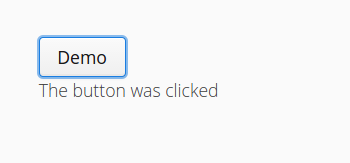
\includegraphics[width=80mm]{Figures/vaadin_democlick.png}
 	\caption{Vaadin Demo Click\label{overflow}}
\end{figure}
Thử nhìn lại nếu chúng ta xây dựng cùng chức năng trên dù là thủ công hay sử dụng các framework Web thông thường thì đều cần phải có một client script đảm nhận việc bắt sự kiện click của người dùng ở browser (front-end) và truyền nó lên server, ngay khi server nhận được (phải có đoạn code ở server "back-end" để xử lý thông tin click truyền lên từ browser), server sẽ trả về thông báo "The button was clicked", rồi front-end javascript phải thêm hay chèn một đoạn text "The button was clicked" vào HTML. Với Vaadin tác vụ vừa mô tả được thực hiện bằng đoạn code trên một cách đơn giản và dễ hiểu hơn rất nhiều.
\subsection{Kiến trúc}
Vaadin hỗ trợ 2 mô hình lập trình: client và server. Mô hình lập trình phía server mạnh mẽ hơn. Mô hình lập trình phía server đảm nhận phần giao diện trên trình duyệt và giao tiếp AJAX giữa trình duyệt và server - hay nói cách khác các giao tiếp giữa server-client nhằm hỗ trợ những thao tác của người dùng đã được xử lý bởi framework và được cài đặt vào bên trong các \textit{Component} của Vaadin. Trong phạm vi ứng dụng mà chúng em xây dựng chỉ sử dụng những thành phần server - chỉ sử dụng các \textit{Component} mà Vaadin cung cấp, cộng với một vài plugin (được viết sẵn cho Vaadin) từ Vaadin Directory \cite{vaadindirectory} để giúp việc phát triển nhanh chóng hơn. 
\\
Hình sau mô tả kiến trúc cơ bản của một ứng dụng web trên Vaadin Framework. Kiến trúc ứng dụng phía server bao gồm nền tảng server (Server-side framework) và hệ thống phía client (Client-side engine). 
\begin{figure}[ht!]
	\centering
	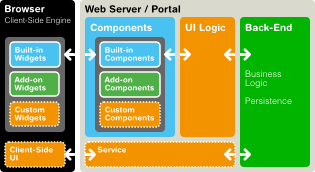
\includegraphics[width=100mm]{Figures/vaadin_architecture0.png}
	\caption{Kiến trúc của Vaadin\label{overflow}}
\end{figure}

\subsubsection{Web Server}
\begin{description}
\item[Components] Các \textit{Built-in Components}, \textit{Add-on Components} đều là những thành phần được xây dựng sẵn bởi Vaadin hoặc được cung cấp dưới dạng các add-on từ Vaadin Directory \cite{vaadindirectory} nhằm giúp việc phát triển UI nhanh chóng hơn. Chúng đảm nhiệm back-end code để giao tiếp với các \textit{Built-in Widgets}, \textit{Add-on Widgets} ở phía browser (client side).
\item[UI Logic, Service và Custom Components] là những phần mà lập trình viên phải tự viết code để cài đặt các tác vụ tương tác mà họ mong muốn, tuy nhiên Vaadin cũng cung cấp các abstract class, interface để hỗ trợ việc này. 
\item[Back-end] Trong một ứng dụng thông thường thì đây chính là nơi để xử lý giao tiếp với các đối tượng trong cơ sở dữ liệu - nơi thực hiện các thao tác Create Read Update Delete (CRUD).
\end{description}
\subsubsection{Client-Side Engine}
\begin{description}
\item[Built-in Widgets] Đây chính là thành phần Client-side của \textit{Built-in Components} đảm nhiệm bắt các sự kiện của người dùng với browser và giao tiếp với các \textit{Built-in Components} ở server.
\item[Add-on Widgets] là client-side của \textit{Add-on Components}.
\item[Custom-Widgets] là client-side của \textit{Custom Components}.
\end{description}
Toàn bộ các thành phần ở Client-side Engine đều được xây dựng bằng JavaScript. Đây là một ưu thế so với các nền tảng trên Flash, Java Applets hay các plugins khác. Vaadin dựa trên sự hỗ trợ của Google Web Toolkit cho nhiều trình duyệt khác nhau, nên lập trình viên không cần lo lắng về sự tương thích của các trình duyệt cho ứng dụng của mình.
\\
Như đã nói ở trên, không giống với các framework web khác là tách biệt front-end và back-end thành 2 phần riêng biệt, Vaadin làm điều ngược lại đó là đem cả hai thành phần đó tích hợp vào \textit{Vaadin Components}, ở hình trên chúng ta sẽ thấy một \textit{Vaadin Component} sẽ gồm một \textit{Widget} ở client-side  và một \textit{Component} tương ứng ở server side. Phân tích ví dụ Demo Click ở bên trên :
\begin{itemize}
\item \textbf{Vaadin Component} chính là một Vaadin Component.
\item \textbf{UILogic} chính là \textit{layout.addComponent(new Label("The button was clicked"));}
\end{itemize}

Tóm tắt lại, Vaadin cung cấp sẵn gần như đầy đủ mọi thành phần UI chúng ta cần để phát triển một ứng dụng web tương tác tốt với người dùng một cách nhanh chóng và tiện lợi. Chúng ta sẽ giảm bớt được công việc khi phải viết Javascript, HTML cho cliend-side khi sử dụng các Vaadin UI Components.
\\
Tuy là tích hợp mọi thứ vào UI components của mình, Vaadin tách biệt UI Logic với các thiết kế giao diện. Điều này đồng nghĩa bên cạnh một giao diện mặc định rất tốt của Vaadin chúng ta có thể thiết kế giao diện một cách dễ dàng thông qua các file CSS hoặc cũng có thể tự định nghĩa HTML Template cho riêng mình \textsuperscript{*}. 
{\let\thefootnote\relax\footnotetext{*\textit{
			Vaadin Theme: https://vaadin.com/book/-/page/themes.html}}
}
\subsection{Vaadin UI Components}
Như đã được nhắc đến nhiều lần trong mục trước, Vaadin UI Component chính là những thành phần tạo nên Vaadin và đơn giản hoá rất nhiều công việc khi chúng ta phát triển ứng dụng web. Dưới đây chúng em xin được nêu lên những thành phần đáng chú ý nhất. Đầu tiên xin giới thiệu thành phần quan trong nhất.

\subsubsection{User Interface} 
\paragraph{Chức năng} Ứng dụng Vaadin cung cấp một giao diện người dùng để lập trình viên có thể mở rộng ra và phát triển các chức năng mà mình mong muốn. Về mặt kĩ thuật, thành phần này sẽ được đảm nhiệm bởi các đối tượng thừa kế từ \textit{com.vaadin.ui.UI} trong source code.
\paragraph{Nhiệm vụ} Khởi tạo lớp UI, từ đây lớp UI sẽ đảm nhiệm các công việc như nạp tất cả UI Components được khai báo bên trong, cài đặt các event listener để tiếp nhận thao tác từ người dùng. Cuối cùng UI được load lên trình duyệt bằng URL, hoặc được nhúng 
vào bất kì trang HTML nào \cite{vaadinarchitecture}.


\subsection{Các UI Component đáng chú ý}
Dưới đây chúng em xin được liệt kê các Components được chúng em sử dụng nhiều trong việc phát triển ứng dụng OWLEditor.
\begin{figure}[h!]
	\centering
	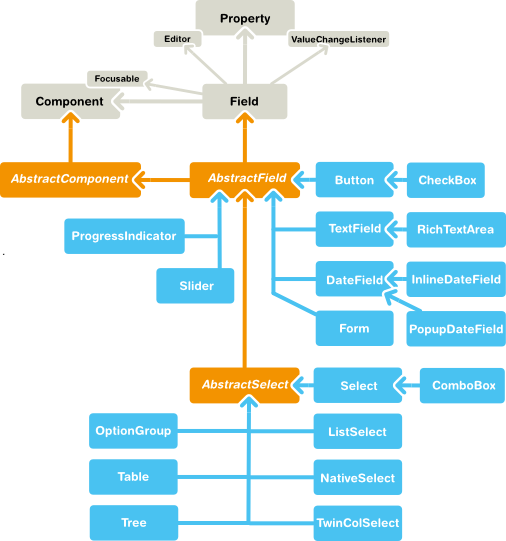
\includegraphics[width=120mm]{Figures/vaadin_architecture1.png}
	\caption{Các UI Components của Vaadin\label{overflow}}
\end{figure}
\subsubsection{Layout}
Vaadin cung cấp nhiều dạng layout khác nhau để hỗ trợ việc tổ chức các components bên trong một cách khoa học, gọn gàng. \cite{vaadinbook}
\begin{description}
\item[HorizontalLayout] tổ chức các components theo chiều ngang, các component được sắp xếp từ trái qua phải.
\item[VerticalLayout] tổ chức các components theo chiều dọc, các component được sắp xếp từ trên xuống.
\item[AbsoluteLayout] tổ chức các components theo đúng vị trí tuyệt đối được khai báo.
\item[CssLayout] tổ chức các components theo định nghĩa từ các file css tương ứng. Đây là cách giúp chúng ta có thể tuỳ chỉnh tối đa bố cục của ứng dụng so với các layout trên.
\end{description} 
\subsubsection{Field Component}
Là những components được thừa kế từ \verb|AbstractField| với chức năng là xử lý các tác vụ input từ người dùng.
\begin{description}
\item[Button] Đảm nhiệm tính năng click từ người dùng, hành động click được xử lý bởi Button.ClickListener và ClickEvent.
\item[CheckBox] Component đảm nhiệm đánh dấu tick từ người dùng, sự kiện được xử lý bởi ValueChangeListener và ValueChangeEvent.
\item[TextField] Đảm nhiệm việc nhập liệu từ người dùng, sự kiện là TextChangeEvent được xử lý bởi TextChangeListener. Hỗ trợ kiểm tra đánh giá input (Validation) cho dữ liệu được nhập vào qua AbstractValidator.
\end{description} 
\subsubsection{Select Component}
Là những components được thừa kế từ \verb|AbstractSelect| với chức năng chính là hiển thị các Data Model (sẽ được đê cập ngay ở mục sau) ra thành các dạng sau.
\begin{description}
\item[Tree] Component cho phép hiển thị Data Model thành dạng cây (ví dụ như cây thư mục), hỗ trợ nhiều tương tác như chọn, thêm, xóa node trên cây.
\item[Table] Component cho phép hiện thị Data Model thành dạng bảng (ví dụ dữ liệu bảng từ SQL Table), hỗ trợ các thao tác như chọn, thêm , xóa dòng trên bảng.
\item[ListSelect] Hiển thị các Data Model theo dạng danh sách, hỗ trợ các thao tác chọn từng dòng, nhiều dòng, thêm dòng và xóa dòng trong danh sách.
\item[ComboBox] Hiện thị các Data Model theo dạng danh sách sổ xuống, hỗ trợ các thao tác như chọn một, thêm dòng mới trong danh sách.
\end{description}
\subsubsection{TabSheet}
\hspace{0.05\textwidth} Tabsheet là một thành phần của Vaadin, là một không gian đa thành phần (multicomponent), có thể chứa nhiều thành phần con bên trong, cho phép chuyển đổi giữa các thành phần bằng cách thay đổi "tab". Các "tab" được sắp xếp như một thanh công cụ luôn nằm ở vị trí cao nhất trong Tabsheet. Khi các "tab" được thay đổi qua lại, thành phần chính của tab đó sẽ trở thành vùng hiển thị chính trên giao diện. Nếu có nhiều tab trong thanh công cụ, các nút điều hướng sẽ được tự động hiển thị. Mỗi tab được xem như là một đối tượng Tab, dùng để quản lý tiêu đề, icon và các thuộc tính khác như ẩn, hiện 
\\
Khi click một tab, Vaadin sẽ kích họat sự kiện TabSheet.SelectedTabChangeEvent, có thể 
được xử lý với interface TabSheet.SelectedTabChangeListener. Thông qua phương thức 
getTabSheet() để lấy được đối tượng tabsheet, và dùng phương thức getSelectedTab() để biết được tab đã được người dùng lựa chọn.

\subsection{Data Model}
Vaadin Data Model cho phép các View (UI components) truy xuất tới dữ liệu một cách trực tiếp, bằng cách cung cấp một interface chuẩn cho mọi loại dữ liệu. Mô hình này cho phép binding các view trực tiếp đến dữ liệu để hiển thị, và cập nhật sự thay đổi ngay lập tức khi dữ liệu được chỉnh sửa. Trong mô hình này có 3 cấp độ cấu trúc khác nhau : property, item và container.
\\
Cần lưu ý rằng Data Model không định nghĩa cách mô tả dữ liệu, mà chỉ định nghĩa interfaces cho việc binding dữ liệu đến các View. Điều này cho phép dữ liệu trong Data Model không bị giới hạn, có thể là các object Java thông thường, đường dẫn hệ thống, hoặc có thể là các câu truy vấn cơ sở dữ liệu.
\\
Data Model được sử dụng rất nhiều trong các component của Vaadin, đặc biệt là các component thừa kế interface Field hoặc AbstractField được đề cập ở mục trên. Một điều thú vị đó là khi tương tác làm cho dữ liệu trong Data Model thay đổi thì dữ liệu hiển thị trên UI Component liên kết với Data Model sẽ tự động được cập nhật. Data Model được tổ chức thành 3 cấp độ khác nhau:
\begin{figure}[h!]
	\centering
	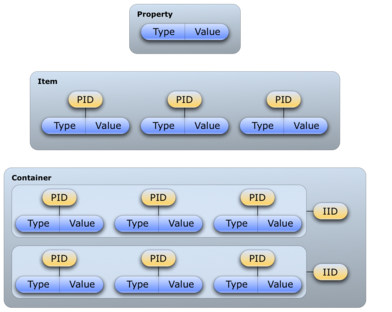
\includegraphics[width=100mm]{Figures/vaadin_datamodel.png}
	\caption{DataModel trong Vaadin\label{overflow}}
\end{figure}
\subsubsection{Properties}
Interface Property là thành phần cơ bản của Vaadin Data Model. Nó cung cấp cho đối tượng dữ liệu các phương thức đọc (get), ghi (set) cơ bản. Kiểu dữ liệu của một property có thể là bất kì lớp Java nào, và nó cũng hỗ trợ chuyển đổi giữa các kiểu dữ liệu.
\begin{itemize}
\item Phương thức setValue() dùng để ghi dữ liệu.
\item Phương thức getValue() dùng để đọc dữ liệu.
\end{itemize}
Các thay đổi của property sẽ kích hoạt sự kiện ValueChangeEvent, và được xử lý bằng ValueChangeListener. Truy xuất đến property bằng cách gọi phương thức getProperty() của event. Property thường không có định danh riêng. Chỉ khi chúng được chứa trong Item, chúng sẽ được định danh bằng các PID (Property Identifier). Tương tự, khi các Item được chứa trong Container, chúng sẽ có các định danh là các IID (Item Identifier). Mỗi component đều có một thuộc tính dùng để liên kết với nguồn dữ liệu được binding, sử dụng phương thức setPropertyDataSource() để thực hiện liên kết này.
\paragraph{Converter} Khi thực hiện binding, chúng ta sẽ gặp phải trường hợp kiểu dữ liệu của data khác với kiểu dữ liệu của component. Để giải quyết điều này, Vaadin cung cấp interface Converter, cho phép lập trình viên sử dụng để tạo ra các converter tuỳ theo mục đích sử dụng, để chuyển đổi kiểu dữ liệu của data sang kiểu dữ liệu hiển thị được của component. Vaadin cung cấp sẵn một vài converter thông dụng, như chuyển đổi giữa string và integer. Tuy nhiên trong ứng dụng OWLEditor, chúng em đã tự định nghĩa ra các Converter của mình để chuyển đổi giữa String và các đối tượng OWLEnity như OWLClass, OWLObjectProperty. Tất cả converter tự xây dựng được khuyến khich để trong ConverterFactory mà Vaadin cung cấp nhầm tự động phát hiện kiểu dữ liệu của MODEL và PRESENTATION để hệ thống tự động chọn converter thích hợp mà không cần cài đặt converter cho component.
\subsubsection{Item} Item được xem như một tập hợp dùng để chứa và quản lý các property. Mỗi property sẽ được gán định danh PID (Property Identifier) và được truy xuất đến bằng cách gọi phương thức getItemProperty() từ đối tượng Item. Item được xem như tương đương với một đối tượng cơ bản trong lập trình hướng đối tượng, tuy nhiên mở rộng hơn với khả năng xử lý được các sự kiện thay đổi liên quan tới nó. Khi các property trong Item bị thay đổi, Item kích hoạt sự kiện PropertySetChangeEvent được xử lý thông qua interface PropertySetChangeListener .
\subsubsection{Container}
Container là cấp cao nhất của mô hình dữ liệu Vaadin ( Vaadin Data Model ), chứa đựng và quản lý các item, trong các item lại chứa đựng và quản lý các property. Container hiển thị dữ liệu dưới dạng cấu trúc, như các dữ liệu thường thấy trong các bảng (Table), hay cây (Tree). Các item trong container được định dang bằng IID (Item Identifier), và các property trong item được định dang bằng PID (Property Identifier).

\chapter{Xây dựng hệ thống phân loại tự động}
\paragraph{Giới thiệu} Qua các chương trước, chúng em đã trình bày các cơ sở lý thuyết gồm OWL 2, SWRL, đề ra các thiết kế cho hệ thống và thiết kế một ontology sử dụng cho việc phân loại. Trong chương này, chúng em sẽ trình bày lại quá trình xây dựng hệ thống phân loại dựa trên các thiết kế ở chương trước.
\section{UI của ứng dụng - OWLEditorUI}
\subsection{Giới thiệu OWLEditorUI}
Lớp này được mở rộng từ lớp \textbf{UI} của Vaadin - chức năng cơ bản của \textbf{UI} là nơi khởi tạo mọi thành phần giao diện và trình bày nó dưới dạng HTML trên web page, OWLEditorUI mở rộng các chức năng trên như sau:
\begin{itemize}
\item Chứa EntryView, MainView (các View này chứa tất cả thành phần giao diện của hệ thống)
\item Cập nhật và cài đặt MainView khi ontology được nạp vào EntryView.
\item Cập nhật trạng thái khi người dùng refresh trang.
\item Nạp (inject) OWLEditorKit và cung cấp nó qua phương thức tĩnh (static).
\item Nạp EventBus và cung cấp qua các phương thức tĩnh.
\item Nạp HttpSession và cung cấp qua phương thức tĩnh .
\end{itemize}
\subsection{Chi tiết các chức năng của OWLEditorUI}
Trước khi đi vào chi tiết các chức năng trên, chúng em muốn giới thiệu khái quát về cách thức hoạt động của Spring Boot \cite{springboot}, các Annotation đáng chú ý được sử dụng trong việc xây dựng hệ thống.
\\
\textbf{Spring Boot} : Khi chương trình khởi động - nghĩa là khi chương trình được nạp vào một hệ thống Servlet như Tomcat, Jetty thì điểm xuất phát đầu tiên của chương trình sẽ từ đối tượng sau:
\begin{verbatim}
@SpringBootApplication public class OWLEditorApplication {
    public static void main(String[] args) {
       SpringApplication.run(OWLEditorApplication.class, args); }
}
\end{verbatim} 
@SpringBootApplication là một tên thay thế cho 3 annotation gồm \textbf{@Configuration}, \textbf{@EnableAutoConfiguration} và \textbf{@ComponentScan} (sẽ được giới thiệu ở dưới), mục tiêu của đối tượng này là khởi động ứng dụng, duyệt hết trong package hiện hành tới package con để tìm các Component Bean cần thiết để khởi tạo và thực thi các Bean đó. Cụ thể ở đây, nó sẽ quét vào tìm thấy \textbf{OWLEditorUI} được đánh dấu bằng \textbf{@VaadinUI} và chạy theo cấu hình có săn được định nghĩa trong Spring 4 Vaadin \cite{spring4vaadin}. Từ đây mọi thứ sẽ diễn ra trong \textbf{OWLEditorUI}. Ý nghĩa của các Annotation:
\begin{itemize}	
\item \textbf{@VaadinUI} Là annotation của Spring 4 Vaadin \cite{spring4vaadin} khai báo một lớp là một Bean và là một Vaadin \textbf{UI} cho hệ thống Spring Boot.
\item \textbf{@VaadinComponent} Là annotation của Spring 4 Vaadin, tương tự annotation @Component của Spring Framework: khai báo đây là một Bean cơ bản nhất cho hệ thống Spring Boot.
\item \textbf{@Repository} Là annotation của Spring Framework, khai báo một đối tượng là một Bean với tính chất là nơi để lấy và khai thác dữ liệu, OWLEditorKit được khai báo bằng annotation này.
\item \textbf{@Autowired} Là annotaion của Spring Framework, dùng nạp tự động các Bean đã được khai báo (bằng các annotation như @VaadinComponent, @Component, @Repository, ...) vào hệ thống, cụ thể chúng em dùng các đối tượng này để nạp OWLEditorKit, HttpSession và OWLEditorEventBus vào OWLEditorUI.
\item \textbf{@Theme} Là annotation của Vaadin dùng để nạp thành phần tùy chỉnh CSS cho toàn bộ giao diện của hệ thống.
\item \textbf{@EnableAutoConfiguration} Là annotation của Spring Boot, bật tính năng cấu hình tự động (mọi cấu hình về DataBase, Base Url,... sẽ ở trạng thái mặc định).
\item \textbf{@ComponentScan} Là annotation của Spring, tự động quét và tìm các Bean từ package hiện hành và khởi tạo chúng.
\item \textbf{@Nonnull} Là annotation từ JSR-305, đảm bảo tham số nhập vào không được null, nếu null tự động throw NullPointerException.
\end{itemize}
\subsubsection{Sử dụng OWLEditorKit trong OWLEditorUI}
Như đã nói sơ qua, thì \textbf{OWLEditorKit} được định nghĩa là một Bean của hệ thống nên khi khởi động nó sẽ được tạo ra nhờ tính năng duyệt Bean vừa giới thiệu. Trong OWLEditorUI, chúng ta sẽ nạp (inject) nó vào OWLEditorUI và tạo một phương thức tĩnh để có thể sử dụng từ các thành phần giao diện như sau:
\begin{verbatim}
@Autowired OWLEditorKit eKit; 
public static OWLEditorKit getOWLEditorKit() {
  ((OWLEditorKit) UI.getCurrent()).eKit; }
\end{verbatim}
Lưu ý: \textit{UI.getCurrent()} là một hàm tiện ích của Vaadin nhằm trả về UI đang chạy hiện hành, trong hệ thống mà chúng em xây dựng chỉ có duy nhất một UI là OWLEditorUI nên sẽ ép kiểu trực tiếp, trong trường hợp có nhiều UI cần lưu ý vấn đề kiểm tra loại UI. Trong source code \cite{owleditorSrc}, chúng em chỉ khai báo Annotation @Repository cho lớp \textit{OWLEditorKitImpl} vậy tại sao @Autowired lại biết mà khởi tạo được ? Câu trả lời là hệ thống sẽ quét và tìm đến các lớp áp dụng interface OWLEditorKit mà có Annotation khai báo để khởi tạo. Để đơn giản ở đây chúng em sẽ dùng hàm khởi tạo mặc định trong OWLEditorKitImpl, ngoài ra còn rất nhiều cách thức @Autowired (hoặc inject) khác có thể tham khảo ở \cite{springboot}.
\subsubsection{Sử dụng OWLEditorEventBus trong OWLEditorUI}
Trong thiết kế chúng em sẽ sử dụng \textit{một} EventBus để xử lý sự kiện cho hệ thống, vì vậy sẽ dễ dàng hơn nếu nó được khởi tạo một lần trong OWLEditorUI và cung cấp dưới dạng phương thức tĩnh. Đầu tiên là cấu trúc của một lớp dùng chứa EventBus thật sự và cách tạo ra các hàm tĩnh.
\begin{verbatim}
@VaadinComponent public class OWLEditorEventBus {
  private final EventBus realEventBus = new EventBus(this); //từ Guava API
  public static void post(@Nonnull final Object event) {
    OWLEditorUI.getGuavaEventBus().realEventBus.post(event);  }
  public static void register(@Nonnull final Object obj) { ... } ...
}
// Trong OWLEditorUI
@Autowired OWLEditorEventBus eventBus;
public static OWLEditorEventBus getGuavaEventBus() {
  ((OWLEditorKit) UI.getCurrent()).eventBus; }
\end{verbatim}
Vậy để sử dụng Guava EventBus trong OWLEditorUI, chỉ cần gọi \textit{OWLEditorUI. getGuavaEventBus} hoặc đơn giản hơn \textit{OWLEditorEventBus. <tên phương thức>}.
\subsubsection{Sử dụng HttpSession trong OWLEditorUI}
Tương tự 2 thành phần trên, HttpSession cũng là một Bean có sẵn của Spring nên chúng ta có thể nạp vào OWLEditorUI và sử dụng như sau:
\begin{verbatim}
@Autowired HttpSession httpSession;
public static HttpSession getHttpSession() {
 return ((OWLEditorUI) getCurrent()).httpSession; }
\end{verbatim}
\subsubsection{Cập nhật trạng thái giữa EntryView và MainView}
\begin{figure}[h!]
	\centering
	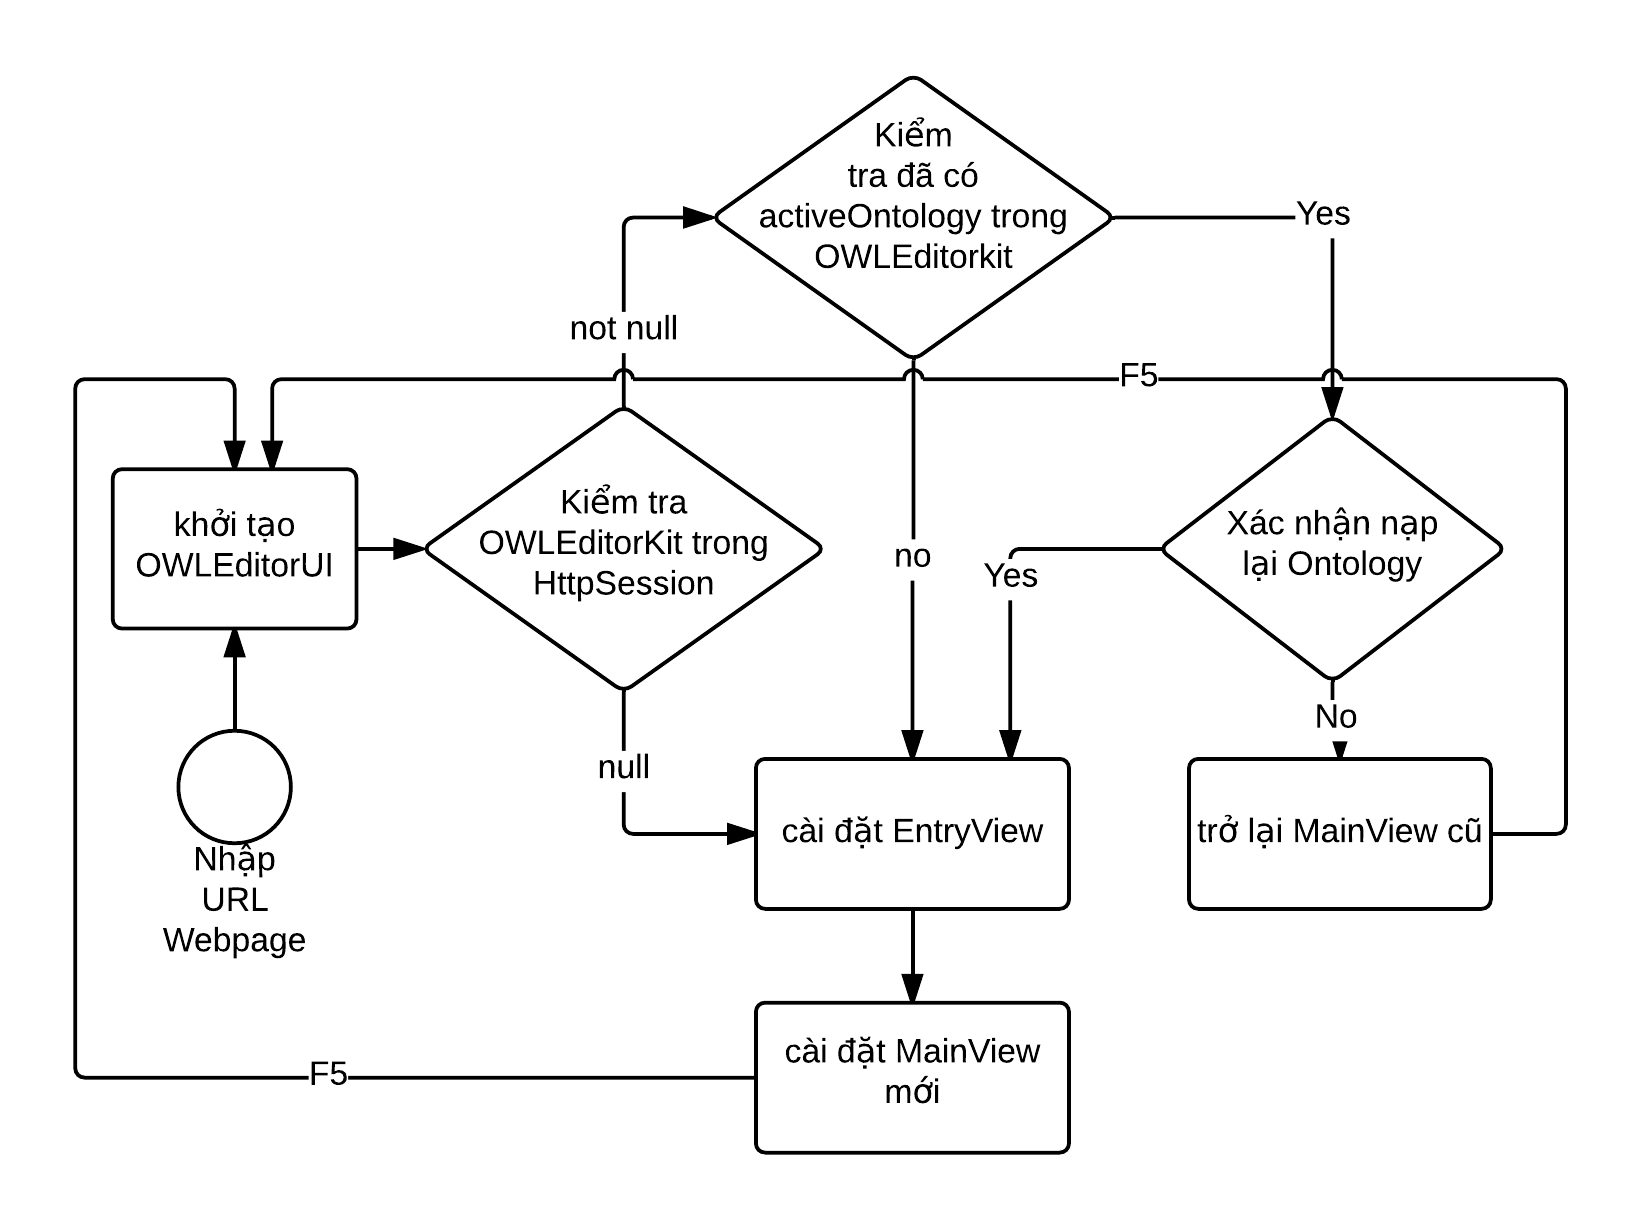
\includegraphics[width=150mm]{Figures/owleditorui_flowchart.png}
	\caption{Vòng đời của các view trong OWLEditorUI \label{overflow}}
\end{figure}
Mỗi lần chúng ta vào trang url của ứng dụng hay refresh thì vòng đời của các View sẽ diễn ra như trong hình 4.1. Việc kiểm tra các điều kiện đều nằm trong phương thức \textbf{updateContent} của OWLEditorUI.
\textbf{Tóm lại} OWLEditorUI là nơi sẽ cung cấp các thành phần lõi của hệ thống như OWLEditorKit, EventBus và HttpSession. Tiếp theo, chúng em sẽ trình bày cách xây dựng các View và thành phần của chúng.
\section{Xây dựng EntryView}
Như được thiết kế thì giao diện của EntryView tương đối đơn giản, chỉ có 1 panel chứa các input để nạp ontology theo 3 tùy chọn:
\begin{enumerate}
\item Nạp ontology qua URL. URL này bắt buộc phải là một tài liệu được định dạng theo tiêu chuẩn OWL 2 (RDF/XML, OWL/XML, FunctionalSyntax/XML,...).
\item Upload một tập tin chứa tài liệu Ontology và nạp tài liệu ontology này vào.
\item Tạo mới một tài liệu ontology.
\end{enumerate}
{\let\thefootnote\relax\footnotetext{
	\begin{enumerate}
		\item \textit{HorizontalLayout} các UI Component được sắp xếp theo chiều ngang, từ trái qua phải.
		\item \textit{VerticalLayout} các UI Component được sắp xếp theo chiều dọc, từ trên xuống.
		\item \textit{AbsoluteLayout} các UI Component được sắp xếp theo đúng vị trí tọa độ được khai báo.
		\item \textit{CssLayout} các UI Component được sắp xếp theo định nghĩa từ các file css tương ứng.
	\end{enumerate}}
}
\begin{figure}[h!]
	\centering
	\frame{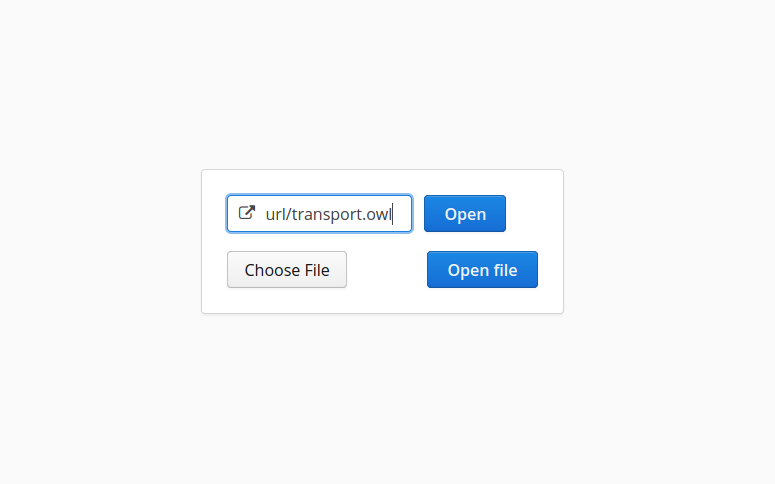
\includegraphics[width=145mm]{Figures/owleditor_entryview.png}}
	\caption{EntryView đã xây dựng\label{overflow}}
\end{figure}
Giao diện EntryView được mở rộng từ layout \textit{VerticalLayout}\textsuperscript{*}, để chứa panel ở giữa - panel này cũng là một \textit{VerticalLayout} tập hợp mỗi dòng là một \textit{HorizontalLayout}, mỗi \textit{HorizontalLayout} này sẽ chứa một \textit{TextField} và một \textit{Button} hoặc một \textit{UploadField} và một \textit{Button} (Hình 4.2) - tất cả các thành phần vừa nêu đều được cung cấp bởi Vaadin. Nhờ vậy, việc xây dựng giao diện khá dễ dàng, chẳng hạn để đặt vị trí trung tâm cho panel trong hình chỉ cần sử dụng dòng code sau :
\begin{verbatim}
setComponentAlignment(entriesPanel, Alignment.MIDDLE_CENTER);
\end{verbatim}
Sau khi click "Open", nếu URL chứa tài liệu hợp lệ thì nó sẽ được nạp vào trong OWLEditorKit, nếu đây là lần đầu OWLEditorKit được sử dụng và chưa được lưu trong HttpSession thì lưu nó vào Session và cuối cùng là chuyển giao diện qua \textit{MainView} (Hình 4.1). Quá trình tương tự cũng xảy ra khi nạp tài liệu từ tập tin upload và tạo mới tài liệu, riêng việc tạo tài liệu thì chúng ta có thể tùy chọn đặt 1 IRI cho nó trong TextField ở dòng cuối. Upload file cũng là một plugin được cung cấp qua \cite{vaadindirectory}, nên việc sử dụng cũng rất đơn giản.
\begin{verbatim}
UploadField uf = new UploadField();
// code bên trong "Open" Button ClickListener
File file = (File) uf.getValue();
OWLEditorUI.getEditorKit() // Nạp ontology vào trong OWLEditorKit
           .loadOntologyFromOntologyDocument(IRI.create(file));
OWLEditorUI.getHttpSession() // lưu OWLEditorKit trong Session
           .setAttribute("OWLEditorKit", OWLEditorUI.getEditorKit());
// Đặt giao diện là MainView 
UI.getCurrent().setContent(new MainView());                    
\end{verbatim}

\section{Xây dựng MainView}
Trong thiết kế \textit{Main}



\chapter{Kết luận}
Với sự phát triển ngày càng nhanh chóng và mạnh mẽ của công nghệ Web 3.0 hay Semantic Web, trong tương lai các hệ thống dữ liệu sẽ sử dụng những nguyên lý của Semantic Web sẽ ngày càng tăng lên do những lợi ích mà nó mang lại so với cách tổ chức dữ liệu truyền thống (Open World vs. Closed World Assumption). Điều này có nghĩa là sẽ có nhiều dữ liệu được tổ chức dưới dạng Ontology Web Language hay các phiên bản RDFS của nó nên việc chúng em đề ra một ý tưởng mới là dùng ontology để phân loại các dữ liệu này là một bước đi đón đầu. Bên cạnh đó, với những lý thuyết về việc sử dụng Ontology cho việc phân loại đã được thực nghiệm trong đề tài, chúng em tin rằng khả năng phát triển một hệ thống thực tế với một ontology với lượng phát biểu lớn về dữ liệu và thông tin của chúng là khả thi và có thể thực hiện bằng các công nghệ hiện tại.
\section{Những công việc đã làm được}
\begin{itemize}
\item Có được những kiến thức nền tảng chắc chắn về ngôn ngữ Ontology Web Language 2, Semantic Web Rule Language và đặc tính suy luận của chúng.
\item Biết được tính nhất quán của ontology  và các nguyên nhân phổ biến gây ra tính thiếu nhất quán trong ontology.
\item Xây dựng được một ứng dụng dùng để thiết kế ontology trên môi trường Web với giao diện thân thiện, dễ dùng và có đầy đủ các tính năng như suy luận, giải thích hỗ trợ biên tập SWRL Rule.
\item Thiết kế môt OWL2 ontology để trình bày tính năng phân loại và tính năng hỗ trợ phân loại từ ứng dụng đã thiết kế.
\end{itemize}
Tóm lại, đề tài nghiên cứu và phát triển "Hệ thống phân loại tự động" đã cho thấy tính khả thi trong việc kết hợp ngôn ngữ Ontology Web Language 2 (OWL2), ngôn ngữ SWRL Rule và cách thức hoạt động của reasoner để phân loại các cá thể một cách tự động. Bên cạnh đó, công cụ chỉnh sửa ontology OWL Editor mà nhóm phát triển đem lại nhiều lợi ích trong việc nghiên cứu và phát triển ontology, cụ thể hơn là đơn giản hoá việc thiết kế một ontology theo ý muốn. Sau khi đạt được những thành công kể trên, đề tài còn có thể đạt được những thành công thực tiễn hơn nếu được áp dụng vào các lĩnh vực khác, chẳng hạn như việc phân loại hàng hoá, hoặc phân loại các gói tin trong lưu lượng mạng...
\section{Những mặt hạn chế}
\begin{itemize}
\item Trình biên tập còn nhiều điểm phản hồi chưa tốt do chúng em chưa chỉ tập trung vào tính năng , vẫn chưa tính đến hiệu năng cũng như hiệu suất của ứng dụng , như việc phải chịu nhiều tải cùng lúc, khả năng lưu trữ, quản lý người dùng.
\item Trình biên tập chưa có cơ chế đăng nhập hoặc quản lý các tài liệu ontology.
\item Ý tưởng về việc phân loại còn chỉ ở dạng mô hình, chưa có tính thực nghiệm cao.
\end{itemize}
\section{Hướng phát triển}
Nhẳm khắc phục một số hạn chế kể trên chúng em cũng đã nghĩ đến các hướng phát triển sau :
\begin{itemize}
\item Để tăng tốc độ xử lý, chúng em sẽ sử dụng kết hơp Vaadin với Spring Boot (đã thực hiện được một phần), đồng thời tố ưu hóa các đoạn code.
\item Trong giai đoạn phát triển cuối cùng, chúng em đã tìm hiểu được là đã có những cơ sở dữ liệu hỗ trợ lưu tài liệu Ontology dưới dạng RDF Graph, tiêu biểu có Stardog - một cơ sở dữ liệu Semantic hỗ trợ OWL 2, SWRL, và đặc biệt tích hợp bản mới nhất của reasoner Pellet 3.0. Sẽ là một ý tưởng tuyệt vời nếu tích hợp sử dụng Stardog là nơi lưu trữ những tài liệu ontology mà người dùng soạn thảo, và giảm tải khả năng suy luận cho cơ sở dữ liệu,
\item Thiết kế một ontology với số lượng lớn các phát biểu phục vụ cho việc phân loại trên thực tế, lĩnh vực là rất rộng lớn nhưng chúng em đã nghĩ đến một lĩnh vực thực tiễn và có thể sử dụng các kiến thức chuyên ngành mạng, đó là phân loại thông tin lưu lượng mạng nhằm phục vụ cho các tác vụ như xây dựng Firewall rule, IDS rule.
\item Đưa ứng dụng thành một ứng dụng mã nguồn mở.
\end{itemize}

Đề tài mà chúng em đã thực hiện, với tính năng phân loại tự động đắt giá, có thể được áp dụng vào nhiều lĩnh vực thực tế khác nhau. Dưới đây là một số ứng dụng có tính khả thi cao :
\begin{itemize}
\item Phân loại các hàng hoá dựa theo các đặc điểm, tính năng đặc trưng của nó
\item Phân loại thông tin lưu lượng mạng nhằm phục vụ cho việc phân tích, ngăn chặn các cuộc tấn công an ninh mạng
\end{itemize}


%% end chapters
\clearpage
%% ----------------------------------------------------------------
% 	Phụ lục 
%% ----------------------------------------------------------------
% Now begin the Appendices, including them as separate files
\addtocontents{toc}{\vspace{2em}} % Add a gap in the Contents, for aesthetics
\appendix % Cue to tell LaTeX that the following 'chapters' are Appendices
\addtocontents{toc}{\vspace{2em}}  % Add a gap in the Contents, for aesthetics
\backmatter
%% ----------------------------------------------------------------
%	Tài liệu tham khảo
%% ----------------------------------------------------------------
\label{Bibliography}
%\lhead{\emph{Tài liệu tham khảo}} 
\bibliographystyle{IEEEtranN}  % Chuẩn IEEE 
\bibliography{Bibliography}  % Tài liệu tham khảo được định nghĩa trong "Bibliography.bib"
%% ----------------------------------------------------------------
\end{document} 
%% ----------------------------------------------------------------
% 	The End
%% -----------------------------------------------------------------
